%% 
%% Copyright 2007-2024 Elsevier Ltd
%% 
%% This file is part of the 'Elsarticle Bundle'.
%% ---------------------------------------------
%% 
%% It may be distributed under the conditions of the LaTeX Project Public
%% License, either version 1.3 of this license or (at your option) any
%% later version.  The latest version of this license is in
%%    http://www.latex-project.org/lppl.txt
%% and version 1.3 or later is part of all distributions of LaTeX
%% version 1999/12/01 or later.
%% 
%% The list of all files belonging to the 'Elsarticle Bundle' is
%% given in the file `manifest.txt'.
%% 
%% Template article for Elsevier's document class `elsarticle'
%% with numbered style bibliographic references
%% SP 2008/03/01
%% $Id: elsarticle-template-num.tex 249 2024-04-06 10:51:24Z rishi $
%%

\documentclass[preprint,12pt]{elsarticle}

%% Use the option review to obtain double line spacing
%% \documentclass[authoryear,preprint,review,12pt]{elsarticle}

%% Use the options 1p,twocolumn; 3p; 3p,twocolumn; 5p; or 5p,twocolumn
%% for a journal layout:
%% \documentclass[final,1p,times]{elsarticle}
%% \documentclass[final,1p,times,twocolumn]{elsarticle}
%% \documentclass[final,3p,times]{elsarticle}
%% \documentclass[final,3p,times,twocolumn]{elsarticle}
%% \documentclass[final,5p,times]{elsarticle}
%% \documentclass[final,5p,times,twocolumn]{elsarticle}

%% For including figures, graphicx.sty has been loaded in
%% elsarticle.cls. If you prefer to use the old commands
%% please give \usepackage{epsfig}

%% The amssymb package provides various useful mathematical symbols
\usepackage{amssymb}
%% The amsmath package provides various useful equation environments.
\usepackage{amsmath}
\usepackage{hyperref}
\usepackage{array} % required for text wrapping in tables
\usepackage{pdflscape} % for landscape table
\usepackage{longtable} % for table going multiple pages
\usepackage{rotating} % for rotated table headers
\usepackage{multirow} % for multi row/col tables
\usepackage{soul} % for highlighting text with \hl 
\usepackage{color} % also required for highlighting 
\usepackage{bibcop} % warnings for incorrect citations
\usepackage[title,titletoc]{appendix} % make it possible to do \ref of an appendix section without automatically getting the word "Appendix"
\usepackage{stmaryrd} % element wise division symbol used in hessian scaling
\usepackage{verbatim} %word counts
%\usepackage{graphicx}
%\usepackage{float}
%\usepackage{placeins}

%% The amsthm package provides extended theorem environments
%% \usepackage{amsthm}

%% The lineno packages adds line numbers. Start line numbering with
%% \begin{linenumbers}, end it with \end{linenumbers}. Or switch it on
%% for the whole article with \linenumbers.
%% \usepackage{lineno}

\newcommand*\rot{\rotatebox{90}} % for rotated table headers
\newcommand{\phant}{\vphantom{\frac{-1}{\rho_M/\rho_w - 1}}} % to make inequality stacks the right height
\newcommand{\matlabFilepath}[1]{figs/2025-04-11_10.21.55/Figure_#1.pdf}
\newcommand{\tableFilepath}[1]{tables/2025-04-11_04.04.45/table_#1.tex}

\newcommand{\summarytexcount}[1]{\textbf{Word Count}
  \immediate\write18{texcount -nosub -inc -sum=[1,1,1,0,0,0,0] -q -brief -template="{title}:\\n   {sum} words, {float} figs/tables, {dsmath} full equations, {inline} inline equations.\\n" #1.tex > #1.wcsum }%
  \verbatiminput{#1.wcsum}%
}
\newcommand{\detailtexcount}[2]{\textbf{Section Breakdown #1}
  \immediate\write18{texcount -sub=#2 -inc -sum=[1,1,1,0,0,0,0] -q -brief -template="{SUB?{title}:\\n {sum} words, {float} figs/tables, {dsmath} full equations, {inline} inline equations.\\n?SUB}\\n" #1.tex > #1.wcdetail }%
  \verbatiminput{#1.wcdetail}
}%

\def\fillandplacepagenumber{% for landscape page numbers
 \par\thispagestyle{empty}%
 \vbox to 0pt{\vss}\vfill
 \vbox to 0pt{\baselineskip0pt
   \hbox to\linewidth{\hss}%
   \baselineskip\footskip
   \hbox to\linewidth{%
     \hfil\thepage\hfil}\vss}}

\journal{Renewable Energy}

\begin{document}

% nominal design
\newcommand{\nominalLCOE}{0.76}
\newcommand{\surgeForceFloatNominal}{2.15}
\newcommand{\surgeForceSparNominal}{0.75}

% min LCOE
\newcommand{\minLCOE}{0.326}
\newcommand{\powerAvgAtMinLCOE}{162}
\newcommand{\powerMaxAtMinLCOE}{295}
\newcommand{\forceMaxAtMinLCOE}{6.42}
\newcommand{\capexAtMinLCOE}{300}
\newcommand{\capexDesignAtMinLCOE}{1.35}
\newcommand{\structMassAtMinLCOE}{$360\cdot10^3$}
\newcommand{\pctImproveLCOEMinLCOE}{57\%}
\newcommand{\pctImproveDesignCostMinLCOE}{37\%}
\newcommand{\pctImprovePowerMinLCOE}{89\%}
\newcommand{\DfoptMinLCOE}{36}
\newcommand{\surgeForceFloatAtMinLCOE}{11.1}
\newcommand{\surgeForceSparAtMinLCOE}{1.09}
\newcommand{\lowestFmaxFactorMinLCOE}{88\%}
\newcommand{\lowestFsatMinLCOE}{64\%}

% min CAPEX
\newcommand{\powerAvgAtMinCapex}{46}
\newcommand{\pctImproveDesignCostMinCapex}{37\%} %(1.35-.853)/1.35
\newcommand{\pctWorsePowerMinCapex}{72\%} %(162-46)/162

% max power
\newcommand{\pctImprovePowerMaxPower}{27\%} %(205-162)/162
\newcommand{\pctWorseDesignCostMaxPower}{14\%}%(1.54-1.35)/1.35

% balanced
\newcommand{\powerBalanced}{140}

% comparison / full pareto
\newcommand{\pctCostSavingsFromPTO}{18\%} % 87 / (87 + 407), using min LCOE and min capex
\newcommand{\powerWhereCusp}{60}
\newcommand{\powerWhereNonconvexEnds}{120} % kW

% sensitivity to model: not optimized
\newcommand{\powerLossForceSatMinLCOE}{2.6} % W
\newcommand{\pctPowerLossForceSatMinLCOE}{0.002\%}
\newcommand{\pctPTOSavingsForceSatMinLCOE}{19\%}
\newcommand{\pctImproveLCOEForceSatMinLCOE}{2\%}

% sensitivity to model: optimized
\newcommand{\pctPowerLossForceSatOptMinLCOE}{0.6\%}
\newcommand{\pctPTOSavingsForceSatOptMinLCOE}{9\%}
\newcommand{\pctStructSavingsForceSatOptMinLCOE}{12\%}
\newcommand{\pctImproveLCOEForceSatOptMinLCOE}{5\%}

% simulation runtime
\newcommand{\simRuntime}{50}
\newcommand{\pctRuntimeMEEM}{76\%}
\newcommand{\pctRuntimeDynamics}{19\%}
\newcommand{\pctRuntimeOther}{5\%}

% formulation
\newcommand{\numLinConstraints}{6}
\newcommand{\numNonlinConstraints}{21}
\newcommand{\numParetoSeeds}{20}
\newcommand{\numParetoSearchPoints}{60}
\newcommand{\numMultistartRequired}{14}

% location sensitivity
\newcommand{\HawaiiDesignCharacteristics}{larger diameter and draft and thinner structural thicknesses}
\newcommand{\LCOEHawaii}{0.579}
\newcommand{\LCOEPacWaveNorth}{0.328}

% optimization runtimes
\newcommand{\singleObjRuntime}{one minute} % 67 seconds on laptop, calkit branch, 6/2/25
\newcommand{\singleObjFcnEvals}{1410}
\newcommand{\singleObjIters}{103}
\newcommand{\paretoRuntime}{seven minutes}
\newcommand{\paretoPctTimeSeeds}{74\%}
\newcommand{\paretoPctTimePatternSearch}{26\%}
\newcommand{\gradientSensRuntime}{under a minute}
\newcommand{\reoptimSensRuntime}{seventeen minutes}
\begin{frontmatter}

%% Title, authors and addresses

%% use the tnoteref command within \title for footnotes;
%% use the tnotetext command for theassociated footnote;
%% use the fnref command within \author or \affiliation for footnotes;
%% use the fntext command for theassociated footnote;
%% use the corref command within \author for corresponding author footnotes;
%% use the cortext command for theassociated footnote;
%% use the ead command for the email address,
%% and the form \ead[url] for the home page:
%% \title{Title\tnoteref{label1}}
%% \tnotetext[label1]{}
%% \author{Name\corref{cor1}\fnref{label2}}
%% \ead{email address}
%% \ead[url]{home page}
%% \fntext[label2]{}
%% \cortext[cor1]{}
%% \affiliation{organization={},
%%             addressline={},
%%             city={},
%%             postcode={},
%%             state={},
%%             country={}}
%% \fntext[label3]{}

\title{Leveraging Multidisciplinary Design Optimization and Semi-Analytical Modeling to Advance Wave Energy Converter Viability}

%% use optional labels to link authors explicitly to addresses:
\author[MAE]{Rebecca McCabe\corref{cor1}}
\ead{rgm222@cornell.edu}
\author[MAE]{Madison Dietrich}
\author[MAE,sys]{Maha Haji}

\cortext[cor1]{Corresponding Author}

\affiliation[MAE]{organization={Sibley School of Mechanical and Aerospace Engineering, Cornell University},
             addressline={124 Hoy Rd.},
             city={Ithaca},
             postcode={14853},
             state={NY},
             country={USA}}

\affiliation[sys]{organization={Department of Systems Engineering, Cornell University},
             addressline={136 Hoy Rd.},
             city={Ithaca},
             postcode={14853},
             state={NY},
             country={USA}}

%% Abstract
\begin{abstract}
%% Text of abstract
Wave energy converters (WECs) can advance the global energy transition by producing clean power for utility grids and offshore technologies.
Considering many disciplines concurrently in an optimization process can allow WEC designers to systematically explore interdisciplinary tradeoffs, more fully capture the breadth of design considerations, and leverage coupling for system-wide benefit.
This paper applies the multidisciplinary design optimization (MDO) methodology to perform single- and multi-objective gradient-based optimization of the Reference Model 3 (RM3), a two-body point absorber WEC design benchmark.
Five hull dimensions, five structural thicknesses, and the generator force and power rating are simultaneously optimized while obeying various static, dynamic, and structural failure constraints.
Objectives include the levelized cost of energy (LCOE), power production, and capital cost.
MDO principles motivate the optimization formulation and solution process.

The optimization's large scope and comprehensive nature are uniquely possible due to the purpose-developed semi-analytical model used for simulation.
The model incorporates a mesh-free eigenfunction-based linear hydrodynamic solver, a quasi-linearized dynamics engine that handles drag and saturation nonlinearities in the frequency-domain, a structural sizing module with realistic yield/ultimate/buckling failure criteria for storm and fatigue design load cases, and a simple cost estimator to assess techno-economic viability.
The text documents the derivation, assumptions, and optimization implications of the model, which is called MDOcean and released open-source.
Validation and computational benchmarking demonstrate that MDOcean's $<50$ms runtime outperforms leading WEC simulation software by orders of magnitude, while maintaining accuracy within a few percent of the baseline in most cases. 

The obtained optimization results achieve a \pctImproveDesignCostMinLCOE~reduction in modeled cost, \pctImprovePowerMinLCOE~increase in power, and resulting \pctImproveLCOEMinLCOE~decrease in LCOE compared to the original RM3 design.
Parameter sensitivity analysis indicates that LCOE depends more strongly on \hl{XX} parameters than \hl{XX} and that the optimal design is sensitive to \hl{XX}.
A Pareto trade-off between cost and power reveals different optimal designs depending on which objective is prioritized, suggesting application-specific design heuristics.
Three representative optimal designs are investigated: a minimum-LCOE design for cost-sensitive operations like utility power, a minimum-cost design for small offshore systems with fixed power needs, and a balanced design for intermediate applications.
\end{abstract}

%%Graphical abstract
\begin{graphicalabstract}
\centering
\includegraphics[width=\linewidth]{\matlabFilepath{45}}
\end{graphicalabstract}

%%Research highlights
\begin{highlights}
\item Develop and validate a rapid ($<\simRuntime$~ms) open-source wave energy simulation incorporating dynamic nonlinearities (generator force saturation, drag), semi-analytical hydrodynamics, and realistic structures (fatigue and storm loadcases, stress and buckling failure modes)
\item Formulate and solve a constrained multi-objective multidisciplinary design optimization with twelve dimensional, structural, and power take-off design variables to maximize power and minimize estimated capital cost
\item Optimal designs achieve up to \pctImproveLCOEMinLCOE~LCOE reduction and tend to have \hl{XX characteristic}
\item Results most sensitive to \hl{XX parameter} and insensitive to \hl{XX parameter}
\end{highlights}

%% Keywords
\begin{keyword}
wave energy conversion \sep marine renewable energy \sep semi-analytical hydrodynamics \sep structural design \sep survivability analysis \sep sensitivity analysis \sep multidisciplinary design optimization \sep techno-economic optimization \sep control co-design \sep two-body point absorber \sep shape optimization \sep power take-off design
%% keywords here, in the form: keyword \sep keyword

%% PACS codes here, in the form: \PACS code \sep code

%% MSC codes here, in the form: \MSC code \sep code
%% or \MSC[2008] code \sep code (2000 is the default)

\end{keyword}

\end{frontmatter}

%% Add \usepackage{lineno} before \begin{document} and uncomment 
%% following line to enable line numbers
%% \linenumbers

%% main text
%%

% added for my convenience, should take out before submission
\tableofcontents
\listoffigures
\listoftables
\clearpage
\summarytexcount{mdocean}
\detailtexcount{sections/model}{subsection}
\detailtexcount{sections/other-appendices}{section}
\newpage

%% Use \section commands to start a section
%% Labels are used to cross-reference an item using \ref command.

\section{Introduction}
\label{intro}
\subsection{Wave Energy Overview}
%(Why WECs, in renewable energy context):

% stronger opening sentence
The global climate crisis requires a transition to carbon-free energy sources such as ocean wave energy.
Ocean waves have higher consistency, predictability, and energy density than other renewable energy sources such as wind and solar, while the temporal complementarity of waves with other resources can improve grid resilience and capacity adequacy, decrease energy prices, and decrease requirements for energy storage and balancing power \cite{akdemir_opportunities_2023,bhattacharya_timing_2021,pennock_temporal_2022}.
Wave energy converters (WECs), the devices that harness and convert this energy, could provide both electricity for the grid at large scale and power for smaller offshore technologies like aquaculture, desalination, and marine sensing \cite{PBE}.
Despite the potential advantages of WECs, a significant decrease in the cost per unit energy production is required before the technology can be deployed at large scales. %\hl{(Add a more specific number to show that the LCOE needs to come down an order of magnitude).} Meanwhile, a lack of design convergence (...)
Thus, a design process that emphasizes techno-economic viability from an early stage is necessary.

%(Why multidisciplinary):
However, the presence of strong interdisciplinary coupling complicates the application of typical design and optimization techniques to WECs.
The powertrain, controller, bulk dimensions, hydrodynamic shape, and structural thicknesses must be selected to balance the complex tradeoff between power production and cost while ensuring survivability and practical feasibility.
Concentrating and automating the design decision-making efforts of structural, control, hydrodynamics, and electrical engineers while accurately capturing all major relationships and requirements is challenging, not to mention computationally prohibitive.
Nonetheless, leveraging the coupling between subsystems and across technical domains can produce large gains in techno-economic viability.
Automating this process through optimization allows WEC designers to more quickly and systematically explore tradeoffs of major design decisions, and could eventually allow standardized comparisons between different WEC architectures.
Thus, performing a system-level WEC optimization that simultaneously considers the coupled techno-economic goals, design decisions, and requirements is highly advantageous.
%Figure~\ref{fig:disciplines} is a non-exhaustive outline of the most common disciplines in a wave energy converter, and the level and direction of coupling between them.

% what is RM3
An initial attempt to consolidate a multidisiplinary WEC design process, though without optimization, was the Reference Model Project.
From 2010 to 2014, the U.S.
Department of Energy funded the creation of six benchmark designs for marine energy devices, published a report \cite{RM3} describing the design considerations and performance calculations, and released design artifacts and other documentation on its website.\footnote{\url{https://openei.org/wiki/PRIMRE/Signature_Projects/Reference_Model}} Three designs are for tidal and current energy turbines, and three are WECs.
The third reference model, known as RM3, is a two-body point absorber WEC designed for a reference site located in Humboldt Bay, California.
The major structural components of the device are a surface float and a spar consisting of a vertical column and a subsurface damping plate, shown in Figure \ref{fig:rm3-parts}.
The float oscillates up and down with oncoming incident waves while the spar stays mostly stationary, and electrical power is produced from this relative heave motion.
\begin{figure}[!ht]%% placement specifier
\centering%% For centre alignment of image.
\includegraphics[width=1\linewidth]{\matlabFilepath{1}}
\caption{RM3 geometry visualized}\label{fig:rm3-parts}
\end{figure}
RM3 has received considerable research attention in the decade since the original report was published.
The present study builds on that work and presents a multidisciplinary techno-economic optimization of the RM3.

The remainder of the introduction will review WEC optimization literature, articulate the appeal of multidisciplinary design optimization to address gaps in the field, and identify the paper's key contributions and structure.

\subsection{WEC Design Optimization: State of the Art and Gaps}
\label{sec:lit}

% design optim / concurrent design in industry
Before reviewing the academic state of the art in WEC optimization, it is worth evaluating the popularity of optimization and concurrent design practices in the wave energy industry.
\cite{trueworthy_wave_2020} provides a critical summary of the WEC design process and shares survey results from 25 WEC designers and developers.
The survey indicates that industry use of optimization techniques is far from universal, with the highest adoption rates at 48\% and 40\% for controls and hydrodynamic shape optimization respectively.
Authors of \cite{trueworthy_wave_2020} speculate that this is due to the large time, expertise, and computational resources needed to perform optimization, the inability of optimization to capture all requirements of a WEC, and the diversity of optimization techniques and design priorities.
A similar rate of 50\% of respondents design all subsystems concurrently.
The others tend to start with the WEC shape and PTO, then move to the controller and moorings, and finish with the power transportation system.
\cite{trueworthy_wave_2020} concludes that concurrent design has promise to take advantage of subsystem interactions and is an under-utilized technique worthy of further study, emphasizing the importance of incorporating all design requirements at an early stage.

% review papers on wec optim
A number of review papers describe the state of the art in WEC design optimization.
Authors of \cite{garcia-teruel_review_2021,guo_geometric_2021} provide overviews of WEC shape optimization, while \cite{ringwood_empowering_2023} reviews wave energy control design, including optimal control and optimization-based control co-design.
On the structures side, \cite{clark_reliability-based_2018} reviews reliability-based design optimization for offshore wind and wave energy, though notably it finds only two examples of WEC structural design optimization.
These two sources \cite{ambuhl_reliability-based_2014, ferri_balancing_2014} will be described further below.
Other references outline relevant guidelines for WEC survivability design without a formal optimization procedure \cite{coe_survey_2018, ove_arup__partners_ltd_structural_2016,paduano_towards_2024,giannini_wave_2022}.

% table summary
Moving on to specific optimization studies, table~\ref{tab:lit} compares the modeling and optimization formulations of a variety of the most relevant examples.
A wide variety of WEC optimizations have been conducted.
After first examining the overall trends, each table entry will be described in more detail.
Point absorbers (PA) seem to be the most common device architecture, though most major device types are represented, and several studies optimize arrays of multiple devices.
Nearly all model hydrodynamics and power production in some way.
Hydrodynamic modeling is typically performed with the boundary element method (BEM), occasionally with semi-analytical models like matched eigenfunction expansion method (MEEM), and rarely with high fidelity CFD.
Dynamic modeling is frequently performed both in the frequency domain (F) and time domain (T), with a handful of studies using extensions of frequency domain techniques (F+) to handle constraints and nonlinearities that are typically only handled in the time domain, and a few using the newer pseudo-spectral method (PS).
A range of controllers are considered, including proportional-integral / reactive (PI), proportional / pure damping (P), their extensions to incorporate constraints (P+/PI+), nonlinear structured (NL), and unstructured (UNS).
Optimizations that incorporate powertrain, structures, and economics are less of a guarantee but still common, while incorporating mooring is relatively rare.
Each discipline may be incorporated with varying levels of fidelity.
It is most common to simulate irregular waves (IRR), though several assume regular waves (REG).
Several incorporate multiple sea states through the use of a joint probability density matrix (IRR+/REG+), and only a few consider storm sea states (STO).
Optimizers used include numerical optimization algorithms like genetic algorithms (GA) and local optimizers (LOC), analytical optimization via Pontryagin's maximum principle (PMP), as well as non-optimization techniques such as design of experiments (DOE), manual iteration (IT), and brute force sweeps (BF).
Objectives are usually power (PWR) or a measure of economic viability or proxy thereof (ECON).
Less common objectives include measures of power variability (VAR), array interaction (ARRY), load (LO), and bandwidth (BW).
The constraints column describes all the requirements the designs are made to satisfy, whether this is achieved with actual optimization constraints or by the simulation model.
Constraint categories include device geometry (GEO), motion amplitude (AMP), the power take-off (PTO), dynamic stability (STA), structural failure (STR), and power (PWR).
The design variables column counts only the optimization decision variables corresponding to an actual design parameter, and not any state variables that may be included in the optimization decisions, such as in the direct transcription or pseudospectral formulations.
Common design variables are bulk dimensions (DIM), hull shape (SHP), and control parameters (CTL).
PTO design variables are common among the pseudo-spectral optimizations, while structural (STR) design variables are rare.
Most studies have fewer than five design variables, with the three largest optimizations having 14, 15, and 66 variables.

%Need to copy sources over from slide 27 and 35 of F24 reseach slides with original charts (with color)

\begin{landscape}
\begingroup
\centering

%\begin{tabular}

\begin{longtable}{>{\centering\arraybackslash}p{0.03\linewidth}|>{\centering\arraybackslash}p{0.05\linewidth}|>{\centering\arraybackslash}p{0.055\linewidth}|>{\centering\arraybackslash}p{0.040\linewidth}|>{\centering\arraybackslash}p{0.015\linewidth}|>{\centering\arraybackslash}p{0.025\linewidth}|>{\centering\arraybackslash}p{0.045\linewidth}|>{\centering\arraybackslash}p{0.045\linewidth}|>{\centering\arraybackslash}p{0.045\linewidth}|>{\centering\arraybackslash}p{0.045\linewidth}|>{\centering\arraybackslash}p{0.055\linewidth}|>{\centering\arraybackslash}p{0.055\linewidth}|>{\centering\arraybackslash}p{0.045\linewidth}|>{\centering\arraybackslash}p{0.055\linewidth}|>{\centering\arraybackslash}p{0.055\linewidth}|>{\centering\arraybackslash}p{0.055\linewidth}|>{\centering\arraybackslash}p{0.02\linewidth}}
\rot{\textbf{Ref}} & \rot{\textbf{Device}} & \rot{\textbf{Hydro}}& \rot{\textbf{Drag}} & \rot{\textbf{\# DOF}} & \rot{\textbf{Domain}} & \rot{\textbf{Controls}} & \rot{\textbf{Mooring}} & \rot{\textbf{Powertrain}} & \rot{\textbf{Structures}} & \rot{\textbf{Economics}} & \rot{\textbf{Sea state}}
& \rot{\textbf{Optimizer}}& \rot{\textbf{Objective}} & \rot{\textbf{Constraints}} & \rot{\textbf{\shortstack{Design \\ Variables}}}& \rot{\textbf{\# DVs}} \\
\hline
This work & 2-PA & MEEM & DF & 1 & F+ & PI+ & - & EFF & AN & STR, PTO & REG+, STO
& LOC & ECON, PWR & GEO, AMP, PTO, STA, STR & DIM, STR, PTO & 12 \\

\cite{mccabe_multidisciplinary_2022} & 2-PA & ALG & - & 1 & F+ & PI+ & - & EFF & AN & STR & REG+, STO
& LOC & ECON, VAR & GEO, PTO & DIM, PTO & 7 \\

\cite{khanal_multi-objective_2024} & 1-PA array & BEM & - & 4 & F & PI+ & - & - & - & GEO & REG
& GA & ECON, ARRY & GEO, PTO & DIM, CTL & 14 \\

\cite{gaudin_single_2021} & 1-PA array & MEEM & - & 120 & F & PI & DES & - & AN & MOOR & IRR+, STO & GA & PWR, ECON & GEO, STR & DIM, CTL & 4 \\

\cite{edwards_optimisation_2022} & 1-PA & BEM & - & 1 & F & P & - & - & - & GEO & REG
& GA & ECON & AMP, GEO, PWR, STA & DIM, SHP & 15 \\

\cite{garcia-teruel_reliability-based_2021}& 1-PA & BEM & LD & 1 & F+ & PI & - & - & LD & - & IRR+
& GA & PWR, LD & AMP, PTO & DIM, SHP & 66 \\

\cite{garcia-teruel_design_2022}& 1-PA & BEM & - & 2 & F+ & PI & - & - & - & - & IRR
& GA & ECON, PWR & AMP, PTO & DIM, SHP & 4 \\

\cite{cotten_multi-objective_2022} & ATN & BEM & - & 10 & F+ & P & - & - & LD & - & IRR+
& GA & ECON, LD & GEO, STA & DIM & 8 \\

\cite{abdulkadir_control_2024} & 1-PA & MEEM & LD & 2 & T & NL P & - & - & - & - & IRR
& GA & PWR & GEO & DIM, SHP, CTL & 8 \\

\cite{housner_numerical_2024} & TRM & BEM & - & 4 & T & PI & DYN & - & - & - & REG
& LOC & PWR & GEO & DIM, SHP, CTL & 3 \\

\cite{al_shami_parameter_2019} & 2-PA & BEM & DF & 2 & F & PI & - & - & - & - & REG
& DOE & PWR, BW & - & DIM, CTL, SHP & 7 \\

\cite{RM3} & 2-PA & BEM & Q & 2 & T & P & DES & - & FEA & FULL & IRR+, STO
& IT & - & - & - & - \\

\cite{mi_multi-scale_2025} & OSW & BEM & Various & 8 & T & PI & DYN, DES & DYN & FEA & FULL & IRR+, STO
& IT & - & - & - & - \\

\cite{an_optimal_2024} & OTP & CFD & CFD & - & T & - & - & - & FEA & - & STO
& ALT & ECON & STR & STR & 4 \\

\cite{ambuhl_reliability-based_2014} & 1-PA & - & Q & - & - & - & DES & - & AN & STR & STO
& BF & ECON & STR, STA & DIM, STR & 3 \\

\cite{nguyen_theoretical_2024} & OSW & MEEM & LD & 1 & F & PI & - & - & LD & - & IRR
& BF & ECON, LD & - & DIM & 2 \\

\cite{ferri_balancing_2014} & 1-PA & BEM & LD & 1 & T & P, PI+, UNS & - & DYN & LD & STR & IRR+
& LOC & PWR, LD & AMP, PTO & CTL & 3 \\

\cite{rosati_control_2023} & OWC & BEM & - & 1 & T & NL P+ & - & EFF & - & PTO & IRR+
& BF & ECON, VAR & PTO & PTO, CTL & 2 \\

\cite{son_performance_2016} & 2-PA & MEEM & LD & 1 & F & P & - & EFF & - & - & REG
& BF & PWR & - & PTO & 2 \\

\cite{gaebele_tpl_2025} & 2-PA & BEM & - & 2 & PS & PI & - & DYN, EFF & - & PTO, GEO & IRR
& LOC & ECON & PTO & PTO, CTL, DIM & 5 \\

\cite{devin_high-dimensional_2024} & 1-PA & FIT & - & 1 & PS & UNS & - & DYN, EFF & - & - & REG
& DOE, BF, LOC & PWR & PTO & PTO, CTL & 5 \\

\cite{grasberger_control_2024} & OSW & BEM & - & 1 & PS & PI & - & DYN & - & GEO & IRR
& BF, LOC & ECON & AMP, PTO & DIM, PTO, CTL & 2 \\

\cite{herber_dynamic_2014} & 1-PA & FIT & LD & 1 & T & UNS & - & - & - & - & IRR& BF, LOC & PWR & AMP, PTO & DIM, CTL & 2 \\

\cite{lin_fast_2025} & 1-PA & BEM & LD & 1 & F+ & UNS & - & - & - & - & IRR+
& BF, PMP & ECON & AMP, PTO & DIM & 1 \\

\cite{abdulkadir_optimal_2024} & 1-PA array & BEM & - & 3 & T & UNS & - & - & - & - & IRR
& PMP & PWR & PTO & CTL & - \\

%\cite{zhang_performance_2024} & 3-PA & MEEM & LD & 3 & F & P & DYN & - & - & - & IRR
%& BF & PWR & - & CTL & 2 \\

%\cite{wen_shape_2018} & 1-PA & BEM & - & 1 & F & P & - & - & - & - & IRR+
%& DOE, LOC & PWR & STA & DIM, SHP & 3 \\

\hline 
%\end{tabular}
\caption{Comparison of previous WEC optimization studies' disciplinary scope, modeling fidelity, and optimization formulation}
\label{tab:lit}
%\fillandplacepagenumber
\end{longtable}
\endgroup
\end{landscape}

\begin{landscape}
\begingroup
\begin{table}
    \centering
    \begin{tabular}{>{\centering\arraybackslash}p{0.05\linewidth}>{\raggedright\arraybackslash}p{0.15\linewidth}|>{\centering\arraybackslash}p{0.05\linewidth}>{\raggedright\arraybackslash}p{0.15\linewidth}|>{\centering\arraybackslash}p{0.05\linewidth}>{\raggedright\arraybackslash}p{0.15\linewidth}|>{\centering\arraybackslash}p{0.05\linewidth}>{\raggedright\arraybackslash}p{0.15\linewidth}|>{\centering\arraybackslash}p{0.05\linewidth}>{\raggedright\arraybackslash}p{0.15\linewidth}}
         \multicolumn{2}{c|}{Device}&  \multicolumn{2}{c|}{Hydro}&  \multicolumn{2}{c|}{Drag} &\multicolumn{2}{c|}{Domain} & \multicolumn{2}{c}{Controls} \\ \hline
         N-PA&  N-body floating point absorber&  MEEM&  Matched eigenfunction expansion method or similar &  DF& Describing function & F&Frequency domain & P&Proportional (pure damping) \\
         ATN&  Attenuator&  BEM&  Boundary element method&  LD& Linear damping & F+&Frequency domain, with extension to incorporate constraints or nonlinearities & PI&Proportional integral (damping and stiffness, aka reactive) \\
         TRM&  Terminator&  CFD&  Computational fluid dynamics&  Q& Quadratic & T&Time domain & P+, PI+&P/PI control with extension to incorporate constraints \\
         OSW&  Oscillating surge WEC&  FIT&  Fit of model to numerical or experimental data&  CFD& Computational fluid dynamics & PS&Pseudo-spectral& NL&Nonlinear structured \\
         OTP&  Overtopping&  ALG&  Algebraic approximation&  &  & & & UNS&Nonlinear unstructured \\
        OWC& Oscillating water column& & & & & & & & \\
    \end{tabular}
    \caption{Legend keys for the dynamics and controls columns of table~\ref{tab:lit}}
    \label{tab:lit-review-legend-dynam}
\end{table}
\endgroup
\end{landscape}

\begin{landscape}
\begingroup
\begin{table}
%    \centering
    \begin{tabular}{>{\centering\arraybackslash}p{0.05\linewidth}>{\raggedright\arraybackslash}p{0.2\linewidth}|>{\centering\arraybackslash}p{0.05\linewidth}>{\raggedright\arraybackslash}p{0.2\linewidth}|>{\centering\arraybackslash}p{0.05\linewidth}>{\raggedright\arraybackslash}p{0.2\linewidth}|>{\centering\arraybackslash}p{0.05\linewidth}>{\raggedright\arraybackslash}p{0.2\linewidth}}
         \multicolumn{2}{c|}{Mooring}& \multicolumn{2}{c|}{Structures} &  \multicolumn{2}{c|}{Economics}&  \multicolumn{2}{c}{Sea state}\\ \hline
         DYN&  Model incorporates mooring dynamics &  AN&  Models stress analytically as a function of dimensions&  STR&  Models structural cost &  REG
& Regular waves\\
         DES&  Study considers mooring physical design &  LO&  Models load without dimension-dependent stress &  PTO&  Models power take-off cost &  IRR
& Irregular wave spectrum\\
         &  &  FEA&  Models stress using finite element analysis &  GEO&  Geometric cost proxy (i.e. hull volume, surface area)&  REG+, IRR+& Joint probabilities of wave heights and periods for multiple sea states\\
         &  &  &  &  FULL&  Full cost model &  STO& Storm condition\\
    \end{tabular}
    \caption{Legend keys for other modeling columns of table~\ref{tab:lit}}
    \label{tab:lit-review-legend-other}
%\end{table}
\bigskip
%\begin{table}
%    \centering
    \begin{tabular}{>{\centering\arraybackslash}p{0.05\linewidth}>{\raggedright\arraybackslash}p{0.2\linewidth}|>{\centering\arraybackslash}p{0.05\linewidth}>{\raggedright\arraybackslash}p{0.2\linewidth}|>{\centering\arraybackslash}p{0.05\linewidth}>{\raggedright\arraybackslash}p{0.2\linewidth}|>{\centering\arraybackslash}p{0.05\linewidth}>{\raggedright\arraybackslash}p{0.2\linewidth}}
         \multicolumn{2}{c|}{Optimization} &  \multicolumn{2}{c|}{Objective} &  \multicolumn{2}{c|}{Constraints} & \multicolumn{2}{c}{Design variables}\\  \hline
         LOC&  Local optimizer (gradient-based, derivative-free)&  
ECON&  Economic metrics or proxies, including power/size ratios&  GEO&  Geometric (volume, inertial, layout)& DIM&Bulk dimensions\\
         GA&  Genetic algorithm&  
PWR&  Power production&  AMP&  Amplitude, stroke& STR&Structural thickness\\
         DOE&  Design of experiments (Monte Carlo, Taguchi)&  
VAR&  Power variability (peak/average, std. dev., capacity factor)&  PTO&  PTO force, power, or electromagnetic feasibility& PTO&Power takeoff\\
         IT&  Iterated by hand&  
ARRY&  Array spacing&  STA&  Stability& CTL&Control parameters\\
 ALT
& Altair Inspire (commercial tool)& LO& Loads (force, force per size)& STR& Structural failure& SHP&Hull shape\\
 BF& Brute force sweep& BW& Bandwidth& PWR& Minimum power& &\\
    \end{tabular}
    \caption{Legend keys for the optimization columns of table~\ref{tab:lit}}
    \label{tab:lit-review-legend-optim}
\end{table}

\endgroup
\end{landscape}


% Prior WEC optimization across discipline
More specifically, a few studies \cite{gaudin_single_2021,khanal_multi-objective_2024,edwards_optimisation_2022,garcia-teruel_reliability-based_2021} perform WEC optimization with several disciplines.
These studies are notable for their large scales of 120 degrees of freedom and 14, 15, and 66 design variables respectively.
\cite{gaudin_single_2021} optimizes an array of 20 submerged cylinders, holding the WEC design constant but optimizing site selection, array layout, and mooring design while considering cable and pile cost as well as pile load capacity.
\cite{khanal_multi-objective_2024} optimizes an array of four cylindrical point absorbers, with 4 modeled disciplines of array layout, hydrodynamics, controls, and economics.
\cite{edwards_optimisation_2022} is a point absorber shape optimization study that minimizes surface area as a cost proxy, accounts for stability constraints, and considers only geometries with power extraction equal to theoretical radiation, amplitude, and steepness limits.
\cite{garcia-teruel_reliability-based_2021}, along with the smaller scale study \cite{garcia-teruel_design_2022} by the same authors, apply multi-objective optimization to trade off power with fatigue load and device volume, respectively.
\cite{cotten_multi-objective_2022} similarly optimizes fatigue load for an attenuator-style WEC with many more degrees of freedom but fewer (8) design variables.
A different 8-variable shape optimization \cite{abdulkadir_control_2024} notably calculates hydrodynamic coefficients via the semi-analytical matched eigenfunction expansion method (MEEM), rather than from boundary element method as is typical, but does not include disciplines beyond hydrodynamics and dynamics/controls.

Regarding optimization algorithm, all seven of these studies \cite{khanal_multi-objective_2024,gaudin_single_2021,edwards_optimisation_2022,garcia-teruel_reliability-based_2021,garcia-teruel_design_2022,cotten_multi-objective_2022,abdulkadir_control_2024} utilize the genetic algorithm, a population-based heuristic method.
The alternative to heuristic methods is local optimization, which lacks the exploratory capability of heuristic methods to avoid getting stuck in local optima, but beneficially leverages any smoothness in the objective and scales well to a large ($>50$) number of design variables \cite{martins_engineering_2022}.
A team at NREL attempted local optimization for a terminator shape study but found they could only reasonably optimize 3 of the intended 13 design variables at a time due to the high computational cost of their time-domain simulation \cite{housner_numerical_2024}.
The previous studies \cite{garcia-teruel_reliability-based_2021,garcia-teruel_design_2022,cotten_multi-objective_2022} avoided this issue by simulating primarily in the frequency domain and using the time domain only to address PTO constraints.
Alternatively, design-of-experiment techniques enable systematic exploration of the design space without the use of traditional optimizers.
For example, \cite{al_shami_parameter_2019} performs a 7 design variable shape optimization with the Taguchi method.

Structural optimization of WECs faces a similar challenge in the high compute time of finite element analysis (FEA).
FEA of WECs is most often performed with manual design iterations, as in \cite{RM3,mi_multi-scale_2025}.
These two studies, while not optimization, are extremely multidisciplinary, encompassing mooring design and detailed economic evaluation in addition to the more common hydrodynamics, powertrain, controls, and structures.
Automating the design process reported there remains a long term vision for WEC MDO.
Notably, one study \cite{an_optimal_2024} performs true optimization of WEC structural FEA using the commercial computer aided engineering software Altair Inspire.
The study examines four design variables, although it keeps the power calculations entirely separate from the structural optimization, neglecting the interdisciplinary coupling.
Another structural optimization does not consider power at all, but is able to perform a brute-force sweep of 3 design variables by using analytical equations for stress and other failure modes \cite{ambuhl_reliability-based_2014}.
Finally, several studies consider structures indirectly by examining the load on the device rather than the stress, e.g. \cite{nguyen_theoretical_2024, ferri_balancing_2014}, or equivalently assuming that stress scales with load and does not depend on any other dimensional design variable, e.g. \cite{garcia-teruel_reliability-based_2021, cotten_multi-objective_2022}.
Like the earlier MEEM study, \cite{nguyen_theoretical_2024} uses the equivalent analytical hydrodynamics in elliptical coordinates for an oscillating surge WEC.

The study \cite{ferri_balancing_2014} is notable because in addition to structural loads, it compares various control schemes and simulates second-order drivetrain dynamics.
The control co-design (CCD) methodology \cite{garcia-sanz_control_2019} emphasizes the importance of considering drivetrain dynamics and generator efficiency due to their strong effect on electrical power generation \cite{coe_useful_2023}.
A number of recent studies \cite{rosati_control_2023,son_performance_2016,anderson_re-imagining_2024,devin_high-dimensional_2024,grasberger_control_2024} simultaneously optimize the PTO with the controller.
\cite{rosati_control_2023} optimizes an OWC and is notable for its comparatively detailed cost modeling and its optimization of both economic and power variability metrics.
\cite{mccabe_multidisciplinary_2022} also optimized power variation, although that study's use of regular waves makes the variation formulation less useful.
Meanwhile, one point absorber PTO optimization \cite{son_performance_2016} is additionally notable for its use of the MEEM method.
\cite{gaebele_tpl_2025} is relevant because it optimizes the dimensional scale and PTO of the RM3 WEC directly using a control co-design approach.
It also efficiently incorporates many time-domain constraints (maximum force, speed, average power, RMS torque, and stroke) while maintaining frequency-domain hydrodynamics via the pseudo-spectral (PS) method, which \cite{devin_high-dimensional_2024,grasberger_control_2024} also use.
\cite{devin_high-dimensional_2024} completes a brute-force PTO optimization with 5 design variables, the highest of any brute force optimization considered here.
This is possible because instead of a five-dimensional sweep, the authors perform ten two-dimensional sweeps around a starting point obtained from an initial monte carlo design-of-experiments.
Finally, \cite{grasberger_control_2024} performs an outer brute-force sweep of two geometric design variables and an inner local optimization of 5 PTO and control design variables for an oscillating surge WEC. 

Other CCD papers optimize WEC dimensions without modeling the PTO.
\cite{herber_dynamic_2014} performs a direct transcription co-optimization of cylinder draft and radius with control.
\cite{lin_fast_2025} introduces a new CCD formulation for constrained control that is even faster than PS.
The method leverages the analytical Pontryagin Maximum Principle (PMP) and performs a case study to optimize a single geometric variable.
A different PMP formulation \cite{abdulkadir_optimal_2024} incorporates PTO-constrained array dynamics, although it has not yet been used for design optimization. 

% results / findings of the work
The results of prior studies provide insight into the level of improvement available with optimization and potential trends in the optimal design.
\cite{edwards_optimisation_2022} found that the axisymmetric geometry with minimum surface area and maximum power is a diamond-like shape that flares out just below the waterline and then back in.
\cite{devin_high-dimensional_2024} found that impedance matching at resonance has a large effect on power and PTO sizing has little effect.
This suggests that if cost were included, it may be preferable to have an undersized PTO that frequently saturates its control force.
This agrees with the conceptual argument of \cite{coe_maybe_2021} and the numerical findings of \cite{mcgilton_optimal_2024}.
The latter shows that reducing the maximum PTO force by 70\% leads only to a 3\% decrease in annual energy production, a trend consistent across two device archetypes (RM3 and RM5), four locations, and several dimensional scales.
The recent RM3 optimization \cite{gaebele_tpl_2025} finds that the device should be scaled down by a factor of 0.55 to a new float diameter of 11~m in order to maximize the power per unit surface area, and that the continuous torque constraint is often active, illustrating the importance of including this constraint in the optimization.
%\hl{Summarize more results of the papers described above - what seems promising to motivate that I will look into it.}

% Previous work optimizing point absorbers
%\hl{elaborate, and add previous work studying RM3}

% Gaps
The literature review reveals that no existing optimization study includes dimensional, structural, and PTO design variables.
The closest are \cite{ambuhl_reliability-based_2014} which includes dimensional and structural, and \cite{grasberger_control_2024} which includes dimensional and PTO.
Furthermore, there is a gap of work that use a scalable optimization framework to trade off power production with survivability in a way that accurately considers stress (including the effect of bulk dimensions, rather than using force as a proxy).
The closest is \cite{rosati_control_2023}, which minimizes a cost proxy that incorporates PTO cost and valve material cost but assumes constant structural material cost.
Given the coupling between these disciplines, a system-level optimization considering them all is needed.
Part of the issue in filling these optimization gaps is the lack of a multidisciplinary WEC simulation platform that is sufficiently fast for optimization.
The popular time-domain hydrodynamics tool WEC-Sim \cite{ruehl_wec-simwec-sim_2024} can become multidisciplinary through the use of integrations like NEMOH/Capytaine (hydrodynamic coefficients), PTO-Sim (electric and hydraulic components), WEC-Sim Applications (optimal control and other useful tools), and MoorDyn (mooring).
However, as \cite{housner_numerical_2024} reveals, it is too slow to use for large-scale optimization.
Meanwhile, the newer pseudospectral tool WecOptTool \cite{coe_initial_2020} is faster and suitable for control co-design, but its disciplines are currently limited to hydrodynamics (via Capytaine) and control, with the ability to easily add custom dynamics like PTO and mooring as needed, and it still can take considerable time for large optimizations.
Finally, several studies note that uncertainty in the cost model may have a significant impact on the results, evidencing the need for sensitivity analysis.

\subsection{Relevance of Multidisciplinary Design Optimization}
%(Why MDO):
Multidisciplinary Design Optimization (MDO) has emerged as a powerful strategy to address such challenges.
MDO is a quantitative methodology to formulate, solve, and interpret the results of complex engineering design problems that involve multiple coupled disciplines \cite{agteMDOAssessmentDirection2009}.
Solutions typically utilize local and global optimization algorithms, and the method emphasizes that comprehensive consideration of the coupling between all disciplines often yields designs that perform better than those found by sequentially optimizing each discipline individually \cite{martinsMultidisciplinaryDesignOptimization2013}.
MDO falls under the umbrella of concurrent design.
When one of the disciplines considered is controls, MDO is a form of control co-design.
MDO originated from the field of structural optimization and is well-established in the aerospace industry and gaining traction in the broader energy industry, especially in floating offshore wind turbines (e.g. \cite{abbas_control_2024,jasa_effectively_2022,patryniak_multidisciplinary_2022}).
While there is a recognized need and growing interest in leveraging concurrent design and control co-design for WECs \cite{mi_multi-scale_2025,ringwood_empowering_2023}, MDO has not yet caught on in the wave energy space, preventing potential techno-economic breakthroughs.
It appears that only two existing studies \cite{mccabe_multidisciplinary_2022,khanal_multi-objective_2024} approach WEC design explicitly from an MDO perspective.
The present study builds directly off \cite{mccabe_multidisciplinary_2022}, a preliminary MDO formulation by the same authors that employs significantly less accurate models and fewer design variables.
\cite{khanal_multi-objective_2024}, which one author also contributed to, includes a Sobol global sensitivity analysis in addition to the basic MDO formulation.
Neither paper provides a comprehensive description of how the MDO approach influences the model development and problem formulation, which this paper intends to outline, while also providing useful results and insights for a much more comprehensive WEC optimization. 

The other papers discussed earlier as being multidisciplinary do not explicitly acknowledge the field of MDO and sometimes do not adhere to the major MDO principle of adequately capturing interdisciplinary coupling in the optimization.
For example, the optimization in \cite{edwards_optimisation_2022} minimizes surface material for only the subset of WEC designs achieving maximum power.
This sub-optimal approach fails to account for the tradeoff between power and cost, since the minimum cost to power ratio may occur at a design that sacrifices some power to achieve significant cost savings.

%(Why semi analytical):

% This section needs some more refining.
% The idea is to explain why having open source semi-analytical multidisciplinary models like MDOcean addresses a bottleneck in WEC development, and provide a frame of reference for interpreting lit review in the next section as being in one of these categories.
% This makes it more clear why I'm citing papers that are all over the place: some just-hydro and some just-controls and some multidisciplinary-but-no-optimization.

MDO can use any kind of simulation model to assess the design's performance, including simple algebraic models, theory-intensive semi-analytical models, and standard numerical models.
Table~\ref{tab:model-types} summarizes the tradeoffs.
\begin{table}
    \centering
    \begin{tabular}{c>{\centering\arraybackslash}p{0.25\linewidth}c>{\centering\arraybackslash}p{0.2\linewidth}} 
         \textbf{Model type}&  \textbf{Expertise required}&  \textbf{Accuracy}&  \textbf{Computational cost}\\ \hline
         \textbf{Algebraic}&  Low&  Low&  Low\\ 
         \textbf{Semi-analytical}&  High&  Med&  Low\\ 
         \textbf{Numerical}&  Med&  Med/High&  High\\ 
    \end{tabular}
    \caption{Comparison of model types}
    \label{tab:model-types}
\end{table}
The authors propose that for early-stage WEC design, MDO with a semi-analytical model is the most beneficial.
Semi-analytical models can be orders of magnitude faster than numerical models, often with minimal sacrifices in accuracy.
This is especially helpful for optimization, where the model must be run many thousands of times.
Additionally, semi-analytical models typically vary smoothly with their inputs and can make it easier to obtain accurate gradients, a feature that is often not the case for fully numerical models that may contain non-differentiable artifacts.
Accurate gradients can also speed up convergence of the optimization and allow it to navigate high-dimension design spaces that would be intractable with heuristic algorithms.

Unfortunately, semi-analytical models are less likely to be available commercially or open-source as numerical models are, and developing them from scratch requires substantial background in mathematics, numerical methods, and the technical domain of the model (for example, hydrodynamics or constrained optimal control).
Often, semi-analytical models remain in the realm of theoretical academics, and ``application'' studies that use them to perform design/optimization usually consider just one discipline and have low practical realism.
This is especially true if the models are closed-source, preventing others besides the model authors from using them.
In the context of WECs, low practical realism usually means studies are limited to mechanical power production, without considering cost and realistic constraints, or perhaps using volume or surface area as a cost proxy.
The design studies with high practical realism tend to use numerical models instead.
As the literature review in table~\ref{tab:lit} revealed, the high computational cost of the numerical models means that often a study is either multidisciplinary without optimization \cite{RM3,mi_multi-scale_2025}, or performs optimization for a single discipline, such as controls, powertrain, or structures, not all at once. 

Of the few studies that perform multidisciplinary optimization, those that use numerical models take many hours to run, especially when using heuristic optimizers, preventing designers from iterating quickly.
For example, the BEM-based 4-WEC array optimization in \cite{khanal_multi-objective_2024} took 36 hours to run on a high-end workstation for only a single frequency.
This type of model is too slow for use in realistic large-scale optimizations.
On the other extreme, \cite{mccabe_multidisciplinary_2022} uses an algebraic hydrodynamic model that runs quickly but lacks sufficient accuracy to draw meaningful design conclusions.
The present paper will combine MDO with semi-analytical models to perform a WEC optimization of unprecedented scope.

\subsection{Paper Contributions and Roadmap}
To addresses the gaps just described, the authors of this paper (1) create a fast, multidisciplinary, and open-source WEC simulation software and (2) use the software to conduct what is believed to be the most comprehensive WEC techno-economic design optimization to date.
The developed software, called MDOcean \cite{mccabe_mdocean_2024}, implements relevant semi-analytical models from various fields, integrates them in a scalable framework for WEC simulation and concurrent optimization, and validates them in a WEC system context.
The multi-objective optimization simultaneously varies dimensional, structural, and PTO design variables of the RM3 WEC in order to balance power production, material cost, and generator cost while obeying a variety of practically-relevant constraints.
A local and partial global sensitivity analysis facilitates understanding of the results' uncertainty and applicability to different scenarios.
In addition to the results' own merit, the framework articulated here is scalable to more design variables and disciplines, and could ultimately enable systematic design optimization of many WEC architectures.

In the following sections, first the methodology for modeling and optimization setup is described in section~\ref{sec:optim-methods}.
Next, the results of single-objective optimization, sensitivity analysis, and multi-objective optimization are shown in section~\ref{sec:results}.
Finally, the authors discuss trends and implications, present three representative optimal designs, and recommend future work in section~\ref{sec:discussion}.

\clearpage
\section{Modeling Methodology}
\label{sec:model}

This paper places considerable emphasis not only on the specific methods used but also on the process to select these methods, informed through a lens of MDO and systems thinking, with the intent to guide readers interested in conducting their own multidisciplinary WEC optimization.
In section~\ref{sec:model-overview}, the research objective and design scope are first used to define a broad problem formulation and module decomposition.
Next, section~\ref{sec:modules} describes the construction of the simulation model.
It develops the assumptions, analysis method, and implementation details of each module based on the appropriate balance of accuracy and speed.
Sections \ref{sec:validation} and \ref{sec:sim-runtime} discuss model validation and runtime benchmarking.
The simulation capabilities and limitations are then combined with the original broad design optimization intent to inform a detailed optimization problem formulation.
In this step, the exact objectives, design variables, constraints, and parameters are selected and outlined in section~\ref{sec:formulation}.
The resulting optimization problem is then characterized and its properties ultimately inform the solution method including algorithm selection, discussed in section~\ref{sec:optim-process}.
Finally, the process is tweaked iteratively until it yields satisfactory results, with noteworthy insights integrated into the relevant sections \ref{sec:model-overview} to \ref{sec:optim-process}.
Figure~\ref{fig:overview-methods} depicts this methodology visually.
\begin{figure}
    \centering
    \includegraphics[width=1\linewidth]{\matlabFilepath{2}}
    \caption{Methodology overview}
    \label{fig:overview-methods}
\end{figure}

\subsection{Overview}
\label{sec:model-overview}
The simulation is broken up into five modules: geometry, hydrodynamics, dynamics and control, structures, and economics.
The geometry module uses both bulk dimensions and structural thicknesses to calculate relevant areas, volumes, masses, measures of center, hydrostatics, and stability margins.
Hydrodynamics uses the bulk dimensions to calculate hydrodynamic coefficients using a semi-analytical method.
The dynamics and control module uses the mass, hydrodynamic coefficients, and generator ratings to determine the loads, response amplitude, and power production using a linear frequency domain model adapted to handle specific nonlinearities including drag and powertrain saturation behavior.
It considers both operational and storm design load cases.
The structures module takes in these loads along with bulk dimensions and structural thicknesses to calculate the stress and factor of safety to various failure criterion.
Finally, the economics module calculates the PTO and structural capital costs from generator ratings and material usage respectively, and combines it with the power matrix to estimate the levelized cost of energy.

The extended design structure matrix (XDSM) diagram in Figure \ref{fig:n2} illustrates the functional interfaces between modules.
XDSM diagrams are standard in MDO, with more details available in \cite{lambe_extensions_2012}.
Variables above and below each module are inputs, and variables to the left and right are outputs.
Design variables are shown in the first row.
The optimizer uses the objective $J$ and constraint $g$ outputs from a simulation run to inform the next iteration of design variables $x$, iterating until ultimately converging to a set of optimal values $x^*$, $J^*$, and $g^*$.
The lack of variables in the lower left portion of the diagram indicates that there is no feedback coupling between modules, so an external solver to enforce consistency is not necessary.
This helps decrease the simulation computation time.
The presence of variables in the upper right of the diagram indicates feed-forward coupling in which the output of one module directly affects subsequent modules.
\begin{figure}
\centering
\includegraphics[width=\linewidth]{\matlabFilepath{3}}
\caption{Simplified $N^2$/XDSM diagram}\label{fig:n2}
\end{figure}
When coupling is \textit{non-monotonic}, concurrent optimization is required to obtain the system optimal design, and optimizing each module sequentially or in parallel would result in a sub-optimal system design.
The WEC coupling here is non-monotonic because perturbing a variable from one module in a certain direction does not necessarily determine the direction of the propagated change in coupling variables, objective, and constraints computed in other modules.
With an objective $J$ of LCOE, for example, while an increase in hydrodynamic damping generally increases power production (beneficial to $J$), it also increases structural loading (detrimental to $g$), and the bulk dimensions required to achieve that higher damping may produce higher stresses (detrimental to $g$) and increase the required structural material (detrimental to $J$).
Thus, it would be sub-optimal to optimize the hydrodynamics module strictly for damping or power production followed by a separate optimization considering structures and economics.
Furthermore, while even in a unified optimization it may be tempting to calculate the structural thicknesses within the structures module as the minimum required to sustain loads without failure, it is important to keep structural thicknesses as design variables because they also contribute to the hydrostatic constraints computed in the geometry module.
If active, these constraints could make the system-level optimum material thickness larger than what is structurally necessary.
Reference~\cite{papalambros_principles_2017} describes the monotonicity checking procedure more fully.
Using a monolithic MDO architecture, in which a single optimizer drives the design of all modules and considers all constraints, addresses this non-monotonic coupling. 

All modules except the dynamics module are explicit, meaning they require no internal iteration to converge.
The dynamics module requires iteration to incorporate nonlinearities into the quasi-linear frequency domain model, shown in the XDSM diagram as the orange box.
The dynamics iteration occurs separately for each outer iteration of the optimizer.
This structure is known as the multiple discipline feasible (MDF) architecture.
In principle, it is possible to remove the dynamics iteration and instead incorporate the nonlinear dynamics as a residual equality constraint within the optimization, which is known as the simultaneous analysis and design (SAND) architecture \cite{martins_multidisciplinary_2013}.
SAND generally decreases the runtime of the simulation (analysis) but requires more optimization iterations, since it is the optimization rather than the simulation that must converge residuals. 
The WecOptTool control co-optimization software pursues the SAND strategy by collocating the dynamics constraints with the pseudo-spectral method \cite{coe_initial_2020}.

Readers familiar with trajectory optimization should note that the choice of MDF versus SAND as an MDO architecture parallels that of shooting versus collocation as a transcription method, in the sense that one chooses to enforce governing equations with simulation versus optimization \cite{underactuated}.
However, in MDO the appropriate decision depends on characteristics of all modules, not merely the module whose governing equations are in question.
As \sectionautorefname~\ref{sec:sim-runtime} will demonstrate, the hydrodynamics module, not dynamics and controls, is the dominant computational cost of the simulation.
This means that even a substantial dynamics speedup represents only a small speedup of the full simulation and is unlikely to outweigh the slowdown of more (hydrodynamics) simulation evaluations.
For this reason, SAND would likely increase the runtime of the full optimization, motivating MDOcean's selection of MDF as the more suitable architecture.
Another advantage of MDF over SAND is that the latter invites the possibility of inconsistent dynamics if the optimization terminates unsuccessfully \cite{martins_multidisciplinary_2013} and requires optimizing a dummy constant objective to perform simulation without optimization.


\subsection{Module Details}
\label{sec:modules}

The five modules (geometry, hydrodynamics, dynamics and controls, structures, and economics) will now be described one at a time.
For notation, unbolded unarrowed variables refer to scalars (e.g. $x$ or $X$), arrowed variables refer to vectors ($\vec{x}$ or $\vec{X}$), and bold variables refer to matrices ($\mathbf{x}$ or $\mathbf{X}$).
For dynamic (time-varying) quantities, the time domain representation is denoted with a lowercase variable ($x(t)$), whereas a hat indicates the complex frequency-domain phasor representation, using the capital variable for magnitude ($\hat{X}(\omega)=\hat{X}=|\hat{X}|e^{i\angle \hat{X}}=Xe^{i\angle \hat{X}}$).
The two connect via $x(t)=\Re(\hat{X}e^{i\omega t})=X\cos(\omega t+\angle\hat{X})$, with $\Re$ indicating the real part.
Dots ($\dot{x}=\Re(\hat{\dot{X}}e^{i\omega t})=\Re(s\hat{X}e^{i\omega t})$) indicate time-derivatives, with Laplace variable $s=i\omega$.

%TC:break Geometry
\subsubsection{Geometry}\label{sec:geom}
The geometry module calculates the submerged volume $V_{sub}$ and structural material volume $V_{struct}$ using standard formulas, and additionally analyzes the WEC's stability and hydrostatic equilibrium.
Figure~\ref{fig:dims} shows the bulk dimensions used to characterize the system. $T$ is used to represent drafts, $h$ heights, and $D$ diameters.
Subscripts $f$, $s$, and $d$ refer to the float, spar, and damping plate respectively.
Marked points include the keel $K$, center of buoyancy $B$, center of gravity $G$, and metacenter $M$, all for the unified float-spar-plate system.
\begin{figure}
\centering
\includegraphics[width=\linewidth]{\matlabFilepath{4}}
\caption{Dimension labeling of system}\label{fig:dims}
\end{figure}
Additional dimensions representing support sizes and thicknesses will be described in the structures section \ref{sec:structures}. 
% add still water line label in figure
Stability requires the metacenter $M$ to be above the center of gravity G.
This distance $GM$ can be calculated \cite{newman}:
\begin{equation}\label{eq:GM}
    GM = KB + BM - KG
\end{equation}
where the centers of buoyancy $KB$ and gravity $KG$ are calculated as a weighted sum of the centroids of each component, using submerged geometry for $KB$ and the full geometry for $KG$.
This assumes an even mass distribution, which is inexact due to the placement of structural material and ballast but suffices as an approximation. $BM$ is a term accounting for the pitch/roll stiffness, equal to the second moment of area about the waterplane divided by the total submerged volume, $BM=\pi D_f^4/(64V_{sub})$ \cite{newman}.

Hydrostatic equilibrium requires the mass of displaced seawater to equal the total mass, for the float and spar separately.
Any discrepancy between the structural mass and the required mass is achieved by adding a ballast mass $m_{bal}$:
\begin{equation}
    m_{bal} = \rho_w V_{sub} - \rho_M V_{struct}
\end{equation}
where $\rho_M$ and $V_{struct}$ are the structural material density and volume respectively.
The ballast mass must be positive to prevent sinking, and there must exist sufficient volume in the hull to hold this ballast.
Assuming seawater ballast, a common choice due to its zero cost and operational convenience to enable at-sea ballasting, this becomes:

\begin{equation}\label{eq:vol-constraint}
\begin{aligned}0 &\le{}\\ \implies \frac{-1}{\rho_M/\rho_w - 1}(V_{surf}-V_{pto}) &\le{} \end{aligned}\!
\begin{gathered} m_{bal}\\ \phant V_{struct} \end{gathered}\!
\begin{aligned}{}&\le{}\rho_w (V_{surf}+V_{sub}-V_{struct}-V_{pto})\\ &\le {}\phant \frac{\rho_w}{\rho_M} V_{sub} \end{aligned}
\end{equation}
where $V_{surf}$ is the bulk component volume above the surface and $V_{pto}$ is the PTO volume, assumed constant at its nominal value. %The resulting lower bound on $V_{struct}$ can be removed since it is trivially satisfied for structural materials denser than water, which is assumed here.

%TC:break Hydrodynamic Coefficients
\subsubsection{Hydrodynamic Coefficients}\label{sec:meem}
A regular water wave with height $H$, wavenumber $k$, and frequency $\omega$ that propagates along direction coordinate $+y$ is described by its free-surface elevation $\eta$,
\begin{equation}
    \eta(y,t)=\frac{H}{2}\cos(-ky+\omega t)
\end{equation}
and the position-independent variable $\zeta(t)=\eta(0,t)$ describes the wave elevation at $y=0$.
The first-order hydrodynamic forces $\vec{\hat{F}}$ on a group of interacting floating bodies are expressed using linear wave theory in the frequency domain as:
\setlength\arraycolsep{0pt}
\newcolumntype{C}{>{{}}c<{{}}}
\begin{equation}\label{eq:hydro-forces}
\begin{array}{rCCCCC}
     \vec{\hat{F}} = & \underbrace{\vec{\hat{F}}_{e}}_{\substack{\textrm{wave} \\  \textrm{excitation} }} & +\underbrace{\vec{\hat{F}}_{rad}}_{\substack{\text{hydrodynamic} \\ \text{radiation} }} +&  \underbrace{ \vec{\hat{F}}_{res}}_{\substack{\textrm{hydrostatic} \\ \text{restoring} }} \\
    = & \overbrace{\vec{\hat{\gamma}} \hat{\zeta}} & \overbrace{-\mathbf{A_h}\vec{\hat{\ddot{\xi}}} - \mathbf{B_h}\vec{\hat{\dot{\xi}}}} &  \overbrace{-\mathbf{K_h}\vec{\hat{\xi}}}
\end{array}
\end{equation}
where $\vec{\hat{\xi}}$ represents the body displacements, and hydrodynamic coefficients $\vec{\hat{\gamma}}$, $\mathbf{A_h}$, $\mathbf{B_h}$, and $\mathbf{K_h}$ denote the wave excitation vector, added mass matrix, radiation damping matrix, and restoring force matrix, respectively.
The origin is chosen here as the center of the float.
The full equation of motion incorporating the effect of additional forces will be given in section~\ref{sec:dynamics}.

For a two body point absorber oscillating in heave under normal operational conditions ($op$), the hydrodynamic matrices are 2x2, representing the float $f$, spar $s$, and coupling between the two $c$:
\begin{equation}
    \vec{\hat{\xi}}_{op} = \begin{bmatrix}
        \hat{X}_f \\ \hat{X}_s
    \end{bmatrix},~
    \vec{\hat{\gamma}}_{op} = \begin{bmatrix}
        \hat{\gamma}_f \\ \hat{\gamma}_s
    \end{bmatrix},~
    \mathbf{A_{h,op}} = \begin{bmatrix}
        A_f & A_c \\ A_c & A_s
    \end{bmatrix},~ 
    \mathbf{B_{h,op}} = \begin{bmatrix}
        B_f & B_c \\ B_c & B_s
    \end{bmatrix},~
    \mathbf{K_{h,op}} = \begin{bmatrix}
        K_f & 0\\ 0 & K_s
    \end{bmatrix}
\end{equation}
The coupling is symmetric for radiation forces and zero for hydrostatic forces.
Meanwhile, the hydrodynamic coefficients may change in storm conditions, such as if the devices change their shape or submersion depth as a survival strategy.
The assumed storm configuration in this study, to mirror the RM3 report \cite{RM3}, is the float and spar rigidly fixed to each other so they move as if they have been merged $m$:
\begin{equation}
    \vec{\hat{\xi}}_{storm} = \begin{bmatrix}
        \hat{X}_m 
    \end{bmatrix},~\vec{\hat{\gamma}}_{storm} = \begin{bmatrix}
        \hat{\gamma}_m
    \end{bmatrix},
    ~\mathbf{A_{h,storm}} = \begin{bmatrix}
        A_m 
    \end{bmatrix},~ \mathbf{B_{h,storm}} = \begin{bmatrix}
        B_m
    \end{bmatrix},~
    \mathbf{K_{h,storm}} = \begin{bmatrix}
        K_m
    \end{bmatrix}
\end{equation}
The question now is the calculation of these different coefficients, postponing discussion on the implication of the operational and storm cases until section~\ref{sec:dynamics}.
The stiffnesses ($K_f$, $K_s$, and $K_m$) are frequency-independent and can be trivially calculated from the diameters (see equation~\eqref{eq:gamma-K}), while the remaining coefficients must be calculated in the frequency domain as a function of device geometry by solving the radiation boundary value problem for the fluid velocity potential.
Traditionally, this is done with a boundary element method (BEM) solver, which meshes the floating bodies and solves a large matrix equation.
In MDOcean, a faster, semi-analytical method that exploits the cylindrical symmetry of the problem is used instead: the Matched Eigenfunction Expansion Method (MEEM).
The MEEM radiation solution for two concentric cylinders oscillating in heave was first presented in \cite{mavrakos_hydrodynamic_2004} and later detailed in \cite{chau_inertia_2013}.
The open-source implementation used in this study is summarized in \appendixname~ \ref{sec:MEEM_details} and further described in \cite{mccabe_open-source_2024,mccabe_investigating_2025,khanal_openflash_2025}.
The present section focuses instead on the high-level capabilities and limitations of the model.

The primary appeal of MEEM is its speed.
While exact runtimes will be discussed in section~\ref{sec:sim-runtime}, timing comparisons indicate more than an order-of-magnitude speedup compared to Capytaine BEM for the same level of convergence.
This removes a large bottleneck from design optimization.
Additional advantages over BEM include lower memory requirements, lack of meshing, and avoiding numerical approximation of the Green's function.

Limitations include shape restrictions and numerical overflow.
Since MEEM is a semi-analytical method, it only applies to specific simple geometries.
The version of MEEM used in this work assumes a dual concentric cylinder shown in \figurename~\ref{fig:meem-geom}.
Therefore, the hydrodynamic calculations for the float coefficients must omit the damping plate and approximate the bottom surface of the float as flat rather than slanted, assumptions which have minor impact and could be lifted in future work with a more complicated MEEM formulation, as in \cite{olaya_hydrodynamic_2015,kokkinowrachos_behaviour_1986} respectively.
\begin{figure}
    \centering
    \includegraphics[width=1\linewidth]{\matlabFilepath{5}}
    \caption{MEEM geometry.
Dashed lines represent geometry that is neglected in the MEEM calculations}
   \label{fig:meem-geom}
\end{figure}

Because the damping plate has a more substantial impact on the spar coefficients than the float coefficients, the former are found not by using MEEM but by scaling existing solutions that include the damping plate.
\tableautorefname~\ref{tab:hydro-methods} summarizes the methods used to obtain each coefficient.

\begin{table}
    \centering
    \begin{tabular}{cc}
         Coefficient& Method\\ \hline
         $A_f$, $B_f$, $\hat{\gamma}_f$& MEEM\\
         $A_s$& Approximate $\omega\rightarrow\infty$ solution\\
         $A_c$, $B_s$, $B_c$, $\hat{\gamma}_s$& Nominal BEM solution, scaled with $D_d$ and $T_s$\\
    \end{tabular}
    \caption{Method of computing different hydrodynamic coefficients in MDOcean}
    \label{tab:hydro-methods}
\end{table}

%\hl{Describe how I did the WAMIT damping plate scaling for the spar excitation.}

%The MEEM implementation currently cannot take the damping plate into account, and the plate is expected to have a large impact on the spar added mass and damping. Therefore, algebraic approximations of the damping plate coefficients are used instead of the MEEM solution. 
The spar added mass coefficient $A_s$ is approximated as a frequency-independent quantity based on the mass of water displaced in the spherical projection of the plate \cite{philip_damping_2012}:
\begin{equation}
  %  C_m = 1 + \frac{\rho_w D_d^3}{3m_s} \frac{1}{\frac{1}{2}(\frac{D_s}{D_d})^3 - (\frac{D_s}{D_d})^2 + 1} % this is what I had in dev/heave_plate.m but I guess it's less correct
 A_s =\frac{1}{3}\rho_w D_d^3\left(1 - \frac{3}{4}r^2\sqrt{1-r^2} - \frac{1}{4}(1-\sqrt{1-r^2})^2(2+\sqrt{1-r^2})\right)
\end{equation}
where $r=\frac{D_s}{D_d}$.
The trend is shown in \figureautorefname~\ref{fig:spar_added_mass}.
\begin{figure}
    \centering
    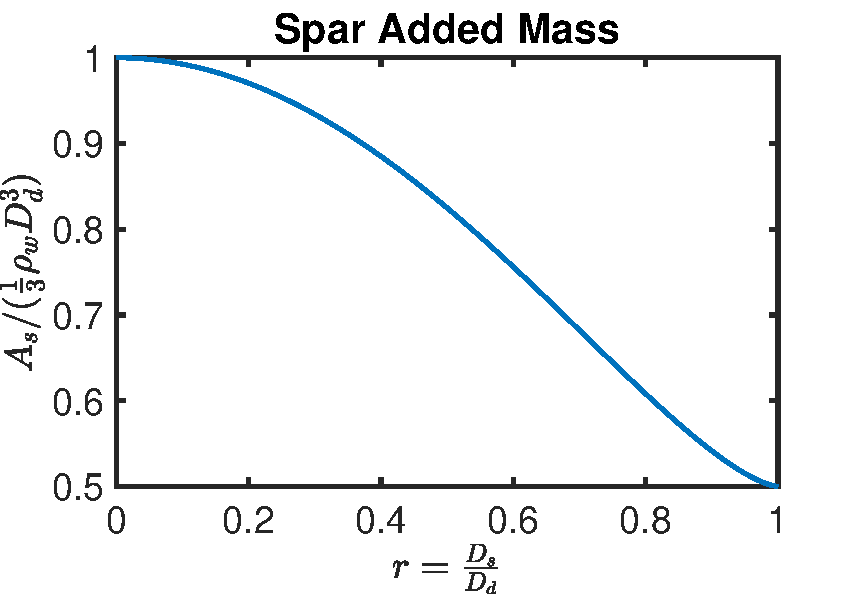
\includegraphics[width=0.5\linewidth]{figs/2025-04-11_10.21.55/Figure_spar_added_mass.pdf}
    \caption{Nondimensional spar added mass as a function of column to damping plate diameter ratio}
    \label{fig:spar_added_mass}
\end{figure}
Meanwhile, the spar damping and excitation ($B_s$ and $\hat{\gamma}_s$) and the coupling damping and added mass ($B_c$ and $A_c$), are obtained by interpolating an existing WAMIT BEM solution for the nominal geometry.
Specifically, interpolation is performed over the nondimensional damping plate diameter $k D_d$.
For $|\hat{\gamma}_s|$, an additional multiplicative factor of $e^{-k (T_s - T_{s,nom})}$ is applied to account for the decrease of excitation with depth.

%  \paragraph{Spar Dynamics}
% The RM3 is a two-body system where the relative motion of the float and spar produces power. However, capturing these underactuated multibody dynamics would require more complicated modeling and control \cite{faedo_principle_2022}, especially in the context of force saturation%, as well as implementation of the excitation force phase in MEEM.
% While updating these models is important future work, a fixed spar is assumed for this study. Thus the results can be considered more dynamically representative of a single-body point absorber or a two-body point absorber with bottom-mounted spar, as might be encountered in shallow water. Nonetheless, calculations still utilize the 45 m water depth of Humboldt Bay, and the results provide relevant preliminary design insights about a floating spar device, especially because the spar structures and economics are still considered. To ensure that the fixed spar assumption is reasonably accurate, the spar amplitude is required to remain small.

% Rather than checking this requirement by calculating the spar amplitude exactly, as this would require the exact modeling complications which the fixed-spar assumption intends to circumvent, the characteristics of second-order linear systems are used to develop a simple sufficient criteria for low spar motion. The peak response amplitude of a system with equation of motion $m\ddot{x}+b\dot{x}+kx=F$ is:
% \begin{equation}
%     |X|_{pk} = \begin{cases}\frac{1}{2\zeta\sqrt{1-\zeta^2}} \frac{F}{m\omega_n^2} & 0<\zeta < 1\\
%     \frac{F}{m\omega_n^2} & \zeta \geq 1
%     \end{cases}
% \end{equation}
% where damping ratio is $\zeta=\frac{b}{2\sqrt{mk}}$ and natural frequency is $\omega_n=\sqrt{\frac{k}{m}}$. To keep the peak spar amplitude $|X|_{pk}$ low, both $\zeta$ and $m\omega_n^2/F=k/F$ should be kept high. A sufficient criteria for maintaining $|X|_{pk}$ below some nominal threshold $|X|_{pk,nom}$ is therefore to constrain $\zeta=\zeta_{nom}$ and $k/F > (k/F)_{nom}$. While this is not a necessary condition (other designs could also maintain low spar amplitude), a sufficient condition is adequate for preliminary optimization purposes. 

% Expressing these conditions in terms of the uncontrolled spar dynamic coefficients \cite{tao_low_2003}:
% \begin{equation}\label{eq:spar}
% \begin{aligned}
% b &= b_{s,rad}+b_{s,drag} \\
% k &= \frac{\pi}{4} \rho_w g  D_s^2 \\
% m &= \rho_w V_{sub,s}C_m\\
%     \omega_n^2 &= \frac{g}{C_m D_d} \frac{1}{\frac{T_s}{D_d} + \frac{h_d}{D_d}\left(\frac{D_d}{D_s}\right)^2} \leq \omega_{n,nom}^2 \\
%     \zeta &= abcd \geq \zeta_{nom}
% \end{aligned}
% \end{equation}
% where $C_m$ is the spar inertia coefficient.

% The geometry is required to maintain at least as high damping ratio and at least as low natural frequency as the nominal RM3 design. While this single-body spar analysis does not take into account the dynamic effect of the PTO force on the spar, it is sufficient to provide confidence that the spar response remains similar enough to the nominal design that the float can be analyzed assuming a fixed spar.

% \hl{Describe the frequency dependent fudge factor and add a figure showing that ratio as a function of sea state.} MDOcean scales the fixed-spar mechanical power by a period-dependent rational tuning factor 
% \begin{equation}
%     P_{spar~floating} = \frac{c_1}{c_2T^2+c_3T+c_4} P_{spar~fixed}
% \end{equation}
% which adjusts only the power (not the amplitude). A fit of MDOcean and RM3 report yielded $[c_1,c_2,c_3,c_4]=[23,1,-15,86]$, and the coefficients can be set to $[1,0,0,1]$ to disable the tuning. 

A second limitation of the present implementation of MEEM is numerical overflow.
To prevent overflow, each fluid region must exceed a minimum height $ \Delta z_{min}$ that is proportional to the region diameter $D$:
\begin{equation}\label{eq:delta-z-min-intro}
    \Delta z_{min} \sim D
\end{equation}
for both the spar ($\Delta z_s, D_s$) and the float ($\Delta z_f, D_f$), with variables shown in \figurename~\ref{fig:meem-geom}.
The constant of proportionality between $\Delta z_{min}$ and $D$ is discussed in \appendixname~\ref{sec:MEEM_details} and is sufficiently small that realistic geometries do not come close to numerical overflow. 

%The current implementation of MEEM yields only the magnitude, not phase, of the excitation coefficient (using equation 99 rather than 97 of \cite{chau_inertia_2012}). Therefore the phase is set to zero, an approximation that will be shown in the following section to be adequate for single body dynamics.

Figure \ref{fig:meem-hydro-coeffs} shows the hydrodynamic coefficients as a function of wave frequency $\omega$ for the nominal RM3 geometry. 
\begin{figure}
\centering
\includegraphics[width=\linewidth]{\matlabFilepath{6}}
\caption{Hydrodynamic coefficients vs. frequency}\label{fig:meem-hydro-coeffs}
\end{figure}
The MEEM results for the simplified cylindrical geometry are a close match to WAMIT BEM results for the exact RM3 geometry, except at frequencies below 0.3 rad/s.
This is expected because the BEM solution assumes infinite depth, which requires a finite added mass at low frequency, whereas MEEM uses finite depth, where the added mass must grow logarithmically toward infinity at zero frequency \cite{mciver_added_1991}.
For the site under consideration, the lowest-frequency sea state containing any energy is 0.4~rad/s, so the discrepancy is not a concern.

%TC:break Dynamics and Control
\subsubsection{Dynamics and Control}\label{sec:dynamics}
\paragraph{Modified Frequency Domain Techniques}
Methods for WEC dynamics and control simulation in an optimization context were reviewed in section~\ref{sec:lit} and include time-stepping (nonlinear, numerical, high computation cost), frequency domain (linear, analytical, low computation cost), pseudo-spectral (nonlinear, numerical, medium computation cost), modified frequency domain techniques (approximate nonlinear, semi-analytical, low computational cost), and Pontryagin's maximum principle (nonlinear, analytical, low computational cost).
MDOcean requires the ability to incorporate nonlinearities, at least approximately.
Inherent nonlinearities such as drag significantly affect the amplitude and power production at resonance.
Even with linearized intrinsic dynamics, maintaining optimality subject to dynamic constraints also requires a nonlinear controller.
Dynamic constraints on amplitude, force, and peak power significantly influence the trade-off of power and cost, and amplitude limits are required to obtain a physically meaningful result.
Besides nonlinearities, MDOcean also requires a low computation cost, since the dynamics will be evaluated many thousands of times during optimization.
Of the methods mentioned, Pontryagin's maximum principle (PMP) and modified frequency domain techniques meet these requirements.
PMP requires an analytically difficult derivation unique to the specific nonlinearities in question because wave energy dynamics have a particular form requiring so-called singular control \cite{zou_optimal_2017}.
On the other hand, modified frequency domain techniques are simple and intuitive.
Therefore, MDOcean pursues a quasi-linear semi-analytical modified frequency domain method.

When handling dynamic constraints with a modified frequency domain method, first the unconstrained optimal controller (and the response signals corresponding to that controller) are determined in the frequency domain.
If the response for a given sea state does not violate any constraints, then the unconstrained controller and corresponding power is used for that sea state.
Otherwise, a variety of approaches are possible to address the violated constraint, summarized in Table~\ref{tab:constraint-approaches} and described below. 

\begin{table}
\centering

\begin{tabular}{>{\raggedright\arraybackslash}p{0.6\linewidth}l l} 
\textbf{Approach} & \textbf{Accuracy} & \textbf{Optimality} \\ \hline
(1) Nonlinear optimal (or near-optimal) controller, linearized via describing functions& High & High \\
(2) Linear optimal controller& High & Medium \\
(3) Saturate or zero the
times with constraint violations, neglecting effect on response& Medium & Medium-low\\
(4) Saturate or zero entire sea state& Low & Low \\
(5) Mark design as infeasible& N/A& Lowest \\

\end{tabular}
\caption{Constraint Satisfaction Approaches for Modified Frequency Domain Methods}
    \label{tab:constraint-approaches}
\end{table}

The modified frequency-domain approach with the highest accuracy and optimality (1) is to synthesize a new nonlinear optimal (or near-optimal) time-domain controller that obeys the constraint, taking into account the linearized effect of that nonlinear controller on the frequency domain response.
If a time-domain PMP control law is available for the constraint under consideration, it can be used as the nonlinear optimal controller directly.
This differs from the standard PMP method in that the response and power corresponding to the time-domain PMP controller is determined in the frequency domain, rather than via numerical time-integration (as in \cite{zou_optimal_2017}) or analytical time-integration (as in \cite{lin_fast_2025}).
For situations without an explicit PMP control law, a nonlinear near-optimal controller can be constructed using insights from signal saturation and filtering, which is the approach pursued here for the force limit.
In either case, the nonlinear controller is linearized via the describing function method.

If a nonlinear controller or the corresponding describing function to linearize it are not available, the most optimal linear controller that obeys the constraint can be used instead (2).
This requires some frequency-domain calculations for an impedance-mismatched linear system described in \cite{mccabe_force-limited_2024} and can be visualized with the Smith chart, a tool common in electrical engineering.
This approach accurately reflects the maximum power that a linear controller could produce, although this power will be lower (less optimal) than that of the optimal nonlinear controller. 

If the implementation for the optimal constrained linear controller is also not available, then the violating portion of the time-domain signals can be saturated or zeroed (3).
This approach neglects the corresponding effect of the saturation/zeroing on other quantities in the system, which lowers the accuracy, and the controller does not have the opportunity to even approximately consider the constraint, resulting in a power production potentially much lower than the constrained optimal.
This simple approach does not require any derivations to implement.
It has been used in several previous WEC optimization studies for various constraints \cite{garcia-teruel_design_2022,garcia-teruel_reliability-based_2021,cotten_multi-objective_2022,mccabe_constrained_2013} and is evidently the most common modified frequency domain method in the marine energy field.
It is utilized here for the power limit.

As a last resort, the energy in that sea state can be zeroed (4), essentially assuming that the device enters survival mode in those cases to avoid constraint violation, or the entire design can be marked infeasible with a constraint in the optimization (5), which \cite{mccabe_constrained_2013} pursues for a radiation limit constraint.
These approaches do not attempt to find dynamic solutions which satisfy the limits, and essentially deal with violations by penalizing the optimization though either the objective or constraints.
The latter approach (5) is actually the only option for slamming amplitude limits in the storm design load case, since the device is already in survival mode and not producing power or applying a control input.
Approach (5) is also pursued here for amplitude limits in the operational design load case, in the interest of consistency and expedience. 

In future work, MDOcean could instead utilize describing functions (1) and the optimal constrained linear controller (2) for the power and operational amplitude limits respectively to improve accuracy and optimality.
The describing function for force saturation is prioritized due to its simpler implementation as well as the force constraint's frequent activity and strong impact on results observed in prior RM3 optimizations \cite{mccabe_multidisciplinary_2022,gaebele_tpl_2025,mcgilton_optimal_2024}.
A describing function (1) is also utilized for the drag nonlinearity.
Table~\ref{tab:nonlinearities} summarizes the dynamic nonlinearities and limits and the method MDOcean currently uses to handle each.

\begin{table}
    \centering
    \begin{tabular}{>{\raggedright\arraybackslash}p{0.25\linewidth}>{\raggedright\arraybackslash}p{0.7\linewidth}}
         \textbf{Dynamic nonlinearity/limit}& \parbox{\linewidth}{\centering\textbf{Method}}\\ \hline
         Drag& Describing function (1) for $\sin(\omega t)|\sin(\omega t)|$ with iteration to find effect on response and optimal controller\\
         Force limit& Describing function (1) for $\text{sat}(\sin(\omega t))$ with iteration to find effect on response and optimal controller\\
         Power limit& Average value of $\text{sat}(\sin(\omega t)+C)$, neglecting any effect on response and optimal controller (3)\\
  Amplitude limit&Optimizer considers limit violations as infeasible designs (5)\\\end{tabular}
    \caption{Dynamic nonlinearities and approach for each}
    \label{tab:nonlinearities}
\end{table}

Describing functions assume a certain time-domain nonlinear signal shape and then calculate the fundamental amplitude of that signal for use in a typical frequency-domain simulation.
For a force signal, the fundamental amplitude is most the relevant harmonic because not only is it typically the largest amplitude, but it undergoes the least amount of filtering by the low-pass plant and therefore contributes the most to power production.
Because the fundamental amplitude depends on the response, the frequency domain simulation is only quasi-linear and must either be iterated numerically or solved analytically.
MDOcean uses iteration to handle both the drag and saturation nonlinearity. % and an analytical solution for the force saturation nonlinearity.

While the describing function method used here has been known for over half a century, MDOcean represents its first application in a wave energy optimization or open-source simulation, to the authors' knowledge.
The RAFT open-source Python package for offshore wind turbines uses the drag describing function with iteration but does not include describing functions for saturation \cite{hall_open-source_2022}.
Thus, MDOcean's semi-analytical dynamics offer a combination of speed, accuracy, and simplicity that is novel in the wave energy space.

\paragraph{Equation of Motion}
The float and spar are each modeled as a floating rigid body, and the two bodies are coupled to transmit force between them.
\hl{Note to scrutineers: the typeset equation below is for a single rigid body (stationary spar), but the actual simulation uses the real two-body dynamics.
The two-body matrix equation will be typeset before submission.} The MDOcean dynamic model assumes %a stationary spar and
regular waves for reasons to be detailed later this section, so the system experiences monochromatic forced oscillation.
The equation of motion can be expressed in the time domain as: % todo: this is time domain so gamma is not allowed to be complex
\setlength\arraycolsep{0pt}
\newcolumntype{C}{>{{}}c<{{}}}
\begin{equation}\label{eq:eom}
\begin{array}{rCCCCC}
     m\ddot{x}(t) = & \underbrace{F_{e}(t)}_{\substack{\textrm{wave} \\  \textrm{excitation} }} & +\underbrace{F_{rad}(t)}_{\substack{\text{hydrodynamic} \\ \text{radiation} }} +&  \underbrace{ F_{res}(t)}_{\substack{\textrm{hydrostatic} \\ \text{restoring} }} &  +~~~~\underbrace{F_{d}(t)}_{\substack{\textrm{drag} }}~~~~+ & \underbrace{F_{p}(t)}_{\substack{\textrm{power}\\\text{takeoff} }} \\
    = & \overbrace{\hat{\gamma}~ \zeta(t)} & \overbrace{-A_h\ddot{x}(t) - B_h\dot{x}(t)} &  \overbrace{-K_hx(t)} & \overbrace{-B_d\dot{x}(t)-K_dx(t)}  & \overbrace{-B_p\dot{x}(t)-K_px(t)}
\end{array}
\end{equation}
where $x(t)$ (body position) and $\zeta(t)$ (wave elevation) were defined in section~\ref{sec:meem}.
Forces include wave excitation, hydrodynamic radiation, hydrostatic restoring, drag, and power takeoff.
For each force component, a linear or quasi-linear model is adopted, with coefficients $\vec{\hat{\gamma}}$, $\mathbf{A_h}$, $\mathbf{B_h}$, $\mathbf{K_h}$ from the hydrodynamics module and $\mathbf{B_d}$, $\mathbf{K_d}$, $\mathbf{B_p}$, and $\mathbf{K_p}$ to be derived in the following sections.
The excitation coefficient $\hat{\gamma}$ is complex, and all other coefficients are real.
In the frequency domain, the complex transfer function from real regular wave height $H$ to complex body amplitude $\hat{X}$ is then:
\begin{equation}\label{eq:eom-freq-domain}
    \frac{\hat{X}}{H} = \frac{\hat{\gamma}/2}{(m+A_h)s^2+(B_h+B_d+B_p)s+(K_h+K_d+K_p)}
\end{equation}
where $s=i\omega$ is the Laplace variable.

\paragraph{PTO Dynamics and Power Production}
A PTO model must capture the dynamics of any elements that transmit, transduce, or condition power between the rigid-body mechanical energy of the float and the end energy product, in this case electricity.
Relevant dynamics include the inertia, stiffness, static friction, mechanical advantage, losses, and electromagnetic coupling of flywheels, shafts, springs, gears, hydraulic circuits, generators, and power electronics.
Reference \cite{penalba_review_2016} reviews common WEC PTO models and \cite{coe_co-design_2024} synthesizes these into a multiport impedance matching network framework to facilitate control co-design.
Reference \cite{coe_co-design_2024} uses the transmission matrix form, which groups the effort and flow variables $e$ and $q$ at each port. 

A linear model of the drivetrain with mechanical transmission matrix $[a]_m$ takes the form
% impedance
% \begin{equation}
% \begin{bmatrix}
% F_p \\ \tau
% \end{bmatrix}
% =
% \underbrace{\begin{bmatrix}
% Z_{m,11} & Z_{m,12} \\
% Z_{m,21} & Z_{m,22}
% \end{bmatrix}}
% _{Z_m}
% \begin{bmatrix}
% \dot{X} \\ \Omega
% \end{bmatrix}
% \end{equation}
\begin{equation}
\begin{bmatrix}
F_p \\ \dot{X}
\end{bmatrix}
=
\underbrace{\begin{bmatrix}
a_{m,11} & a_{m,12} \\
a_{m,21} & a_{m,22}
\end{bmatrix}}
_{[a]_m}
\begin{bmatrix}
 \tau\\ \Omega
\end{bmatrix}
\end{equation}
where the PTO force $F_p$ and WEC velocity $\dot{X}$ are found as a function of the generator torque and rotation speed $\tau$ and $\Omega$.
Meanwhile, linear generator electrical dynamics are expressed with electrical transmission matrix $[a]_e$:
\begin{equation}
\begin{bmatrix}
 \tau\\ \Omega
\end{bmatrix}
=
\underbrace{\begin{bmatrix}
a_{e,11} & a_{e,12} \\
a_{e,21} & a_{e,22}
\end{bmatrix}}
_{[a]_e}
\begin{bmatrix}
 V \\ I
\end{bmatrix}
\end{equation}
with park-transformed quadrature electrical voltage and current $V$ and $I$.
The system operating point is determined by the controller, which is typically formulated at the generator mechanical port.
A linear control law with impedance $\hat{Z}_u$ split into damping and stiffness coefficients $B_u$ and $K_u$ has the form 
\begin{equation}
\tau = \hat{Z}_u \Omega =\left(B_u + \frac{K_u}{s} \right) \Omega
\end{equation}
The time-domain power $P(t)$ at any port is simply the product of the port effort and flow variables.
To facilitate this calculation in transmission form, power can be found as the quadratic product of the port variable vector with the two-dimensional exchange matrix $E_2$,
\begin{equation}
P(t) = e~q
= \frac{1}{2}
\begin{bmatrix}
 e \\ q
\end{bmatrix}^T
\underbrace{\begin{bmatrix}
0~ & 1 \\
1~ & 0
\end{bmatrix}}
_{E_2}
\begin{bmatrix}
 e \\ q
\end{bmatrix}
\end{equation}
where substituting $[e,q]^T=[F_p,\dot{X}]^T$ yields the floating body mechanical power, $[e,q]^T=[\tau,\Omega]^T$ yields the generator mechanical power, and $[e,q]^T=[V,I]^T$ yields the generator electrical power. 

Moving back to the frequency domain and assuming sinusoidal waveforms, the average and peak powers $P_{avg}$ and $P_{pk}$ in a given sea state can be found as:
\begin{equation}
\begin{aligned}
     P_{avg} &= \frac{1}{2}\Re(\hat{e} \hat{q}^*) = \frac{1}{2} \Re(\hat{Z})|\hat{q}|^2 
    \\
    P_{pk} &=  P_{avg} + \frac{1}{2}|\hat{e} \hat{q}^*| = P_{avg}\left( 1 + \sqrt{1 + \left(\frac{\Im(\hat{Z})}{\Re(\hat{Z})}\right) ^2  } \right)
\end{aligned}
\end{equation}
if the port is terminated with complex impedance $\hat{Z}$. 

Rather than utilize detailed PTO models for co-design, which a number of recent papers (e.g. \cite{coe_useful_2023,gaebele_incorporating_2023} and those discussed in section \ref{sec:lit}) have already proven the value of, this study chooses to keep the PTO design unspecified by assuming a constant-gain, infinite bandwidth transmission system and a generator with fixed average efficiency $\eta$.
While obviously unrealistic and insufficient for designing the device's actual PTO hardware, this decision adds simplicity and illustrative value at the system level.
It highlights the effect of the novel non-PTO (e.g. structural) aspects of WEC co-design that this study introduces while still capturing the effect of PTO rating on system performance and maintaining sufficient generality to incorporate more detailed PTO models in the future.
Furthermore, setting $\eta=80\%$ maintains consistency with the RM3 design assumption of \cite{RM3} to facilitate comparison and validation. 

More specifically, rather than implement a full generator electrical transmission matrix $[a]_e$, for the optimization study a simple average efficiency $\eta$ describes the gain between the average mechanical power and average electrical power.
This is not necessarily equivalent to an assumption that the generator itself has constant efficiency, since controllers with reactive terms ($K_u\neq 0$) spend some time expending energy, which reverses the direction of the generator efficiency.
The average efficiency is assumed to also apply to the peak powers, though this is not guaranteed in general for the same reason.
\begin{equation}\label{eq:power-elec}
\begin{bmatrix}
P_{avg,elec} \\
P_{pk,elec}
\end{bmatrix}
= 
\eta
\begin{bmatrix}
P_{avg,mech} \\
P_{pk,mech}
\end{bmatrix}
= 
\eta \frac{1}{2} B_u |\hat{\Omega}|^2
\begin{bmatrix}
1 \\
 1 + \sqrt{1 + \left(\frac{K_u}{B_u \omega }\right) ^2  }
\end{bmatrix}
\end{equation}
Additionally, the drivetrain mechanical transmission matrix $[a]_m$ is set to the identity matrix, which represents a static effective gear radius $R=1$:
\begin{equation}
[a]_m = \begin{bmatrix}
1/R &~ 0 \\
0 &~ R
\end{bmatrix} = \begin{bmatrix}
1 &~ 0 \\
0 &~ 1
\end{bmatrix}
\end{equation}
With this $[a]_m$, the control damping and stiffness $B_u$ and $K_u$ equal the PTO damping and stiffness $B_p$ and $K_p$.
This will simplify the impedance matching procedure described below, requiring matching at only one interface.

%The time-domain mechanical power is $P_{mech}(t) = \tau(t) \Omega(t) = (B_u \Omega(t) + K_u \theta(t) ) \Omega(t) $, where $\theta(t)$ is the generator rotational position. Assuming sinusoidal waveforms, the time-average and peak mechanical power in a given sea state are then

\paragraph{Force-Constrained Optimal Reactive Control}
In the absence of constraints, maximizing absorbed power requires impedance matching.
At the mechanical interface between the floating body and PTO, this means that the force of the PTO on the WEC, described by $F_{p} = B_{p}\dot{X} + K_{p}X$, must have an impedance that is the complex conjugate of the WEC's intrinsic impedance.
This is called reactive control, with subscript $reac$:
\begin{equation}\label{eq:matched-controller}
	B_{p,reac} = B_h + B_d, \qquad K_{p,reac} = (m+A_h) \omega^2 - K_h - K_d
\end{equation}
However, the nominal RM3 design features a hydraulic system which lacks reactive capability (the ability to function as a motor and add energy to the system at some times).
Avoiding reactive power restricts the system to so-called damping control, with subscript $damp$, and requires $K_{p,damp}=0$.
The power-maximizing PTO damping $B_{p,damp}$ is then
\begin{equation}\label{eq:damping-control}
    B_{p,damp} = \sqrt{ (B_{p,reac})^2 + (K_{p,reac}/\omega)^2}
\end{equation}

Both of these controllers frequently result in excessively large generator torques, especially in reactive control when $K_u=K_p$ is far from zero. $K_{p,reac}$ is often a large negative number because cost minimization favors a low mass, and the negative PTO damping reduces the natural frequency to better match the ocean wave frequency with a smaller device mass.
Control laws \eqref{eq:matched-controller} and \eqref{eq:damping-control} provide no mechanism to reduce this torque.
Actuator torque limits are important to model.
Leaving the generator torque unbounded when modeling energetic sea states would result in excessive structural and powertrain requirements.
In response, two strategies are pursued at once: (1) to create an intentional linear impedance mismatch, sacrificing power to satisfy a torque limit, and (2) to use nonlinear control to enable satisfaction of the torque limit with less of a power sacrifice.

Actuator limits change the optimal force signal from a pure sinusoid to a saturated waveform, approaching a square wave for sufficiently low force limit.
As is, this nonlinear signal could not be handled with a frequency-domain transfer function and would require time-domain simulation.
Conveniently, through the describing function method, the saturated signal can be represented with Fourier analysis as a superposition of harmonics.
Furthermore, because the plant is a second order oscillator and filters out high frequency inputs, harmonics other than the fundamental contain very little energy and can be safely neglected.
Figure \ref{fig:sat} shows this approximation graphically for a saturated-sine force signal.
\begin{figure}
\centering
\includegraphics[width=.7\linewidth]{\matlabFilepath{7}}
\caption{Saturated sin vs. time (red) and its fundamental amplitude (blue)}\label{fig:sat}
\end{figure}
Details of the calculation are provided in \appendixname~\ref{sec:appendix-force-sat}.
The result is updated values for control gains $B_u$ and $K_u$ that result in a torque that obeys the force constraint and is used in place of equations~\eqref{eq:matched-controller} and \eqref{eq:damping-control}.

\paragraph{Drag}
Modeling drag force is important to avoid unrealistically high resonant peaks in the response amplitude and the resulting overestimate in power production.
Drag force $F_d$ is proportional to the product of the relative velocity of the WEC and wave, $\dot{x}_{rel}(t)=\dot{x}(t)-\dot{x}_{wave}(t)$, with its absolute value.
The use of the relative velocity rather than direct WEC velocity means that the drag contributes not only a damping-like effect, described with coefficient $B_d$, but also a small stiffness-like effect, with coefficient $K_d$.
The quadratic form $|F_d|\sim|\dot{x}_{rel}|^2$ implies a nonlinear input-output response that would normally require time-domain simulation.
To improve computational efficiency and allow solution in the frequency domain, the nonlinearity is quasi-linearized with another describing function, following \cite{quartier_influence_2021}:
\begin{equation}
\begin{aligned}
    F_{d}(t) &= \frac{1}{2}\rho_w C_d A_w ~\dot{x}_{rel}(t) |\dot{x}_{rel}(t)| \\     
    &= \frac{1}{2}\rho_w C_d A_w ~\dot{X}_{rel}^2 \sin(\omega t) | \sin(\omega t)|\\
    &\approx \frac{1}{2}\rho_w C_d A_w ~\dot{X}_{rel}^2\frac{8}{3\pi} \sin(\omega t)\\
   % F_{d}(\omega)&= \frac{1}{2}\rho_w C_d A_w \frac{1}{2\pi}\dot{X}_{rel}(\omega)*|\dot{X}_{rel}(\omega)| \\
    %\approx  \frac{1}{2}\rho_w C_d A_w \frac{8}{3\pi}  \dot{X}_{rel,1}(\omega)\dot{X}_{rel,1}(\omega) \\
    &= B_{d} \dot{X} + K_{d} X
    \end{aligned}
\end{equation}
with drag coefficient $C_d$.
The nonlinear waveform and describing function approximation are compared in Figure~\ref{fig:drag-df}.
The amplitude of the sinusoidal approximation equals $\frac{8}{3\pi}\approx0.85$ times the peak of the nonlinear waveform.
\begin{figure}
    \centering
    \includegraphics[width=.7\linewidth]{\matlabFilepath{8}}
    \caption{Conceptual demonstration of the drag describing function in the time domain.
The nonlinear signal (red) is approximated by its fundamental amplitude (blue).}
    \label{fig:drag-df}
\end{figure}

The resulting magnitude and phase of WEC motion are obtained by numerically iterating the state-dependent coefficients $B_{d}$ and $K_{d}$.
Further derivation, convergence details, and control implications are discussed in \appendixname~\ref{sec:appendix-drag}.

%\paragraph{Power Saturation}
%Equation~\eqref{eq:mech-power} shows that the power peak to maximum ratio is at minimum two for a damping controller, 
%\hl{describe}

\paragraph{Energy Production}
To find the overall average power production $P_{avg,elec}$ in a location with a given distribution of sea states, $P_{avg,elec}(H,\omega)$ for each sea state is weighted by that sea state's probability using a Joint Probability Density (JPD) matrix.
This method is illustrated in Figure \ref{fig:JPD-muptiply}.
The JPD used in this analysis represents wave conditions in Humboldt Bay, CA and is taken from reference \cite{noauthor_system_2020}.

\begin{figure}
\centering
\includegraphics[width=\linewidth]{\matlabFilepath{9}}
\caption{Power matrices multiplication}
\end{figure}\label{fig:JPD-muptiply}

%As expected, low-frequency sea states achieve mechanical powers close to the radiation limit (device capture efficiencies near one), and high frequency sea states achieve mechanical powers equal to the amplitude limit.

The annual energy production $AEP$ in kWh/year is the product of the number of devices, the average power per device, an efficiency $\eta_{array}$ representing transmission losses and array downtime, and an appropriate constant to convert from Watts to kWh/year:
\begin{equation}
    AEP = N_{WEC} ~ P_{avg,elec} ~\eta_{array} \frac{8766}{1000}
\end{equation}

%Finally, the standard deviation $\sigma$ of power across all sea states $P(\omega)$ is computed, and normalized by the average power $\mu$ to get the coefficient of variation (see equation \eqref{cv}).

\paragraph{Dynamic Limits and Design Load Cases}
This study considers two design load cases: (1) cyclic operational loading in sea states where power is produced, and (2) storm loading in sea states where the device enters survival mode and stops producing power.
These correspond roughly with the 1-year and 50-year return periods specified in the wave energy design standard IEC TS 62600-2, and with the fatigue limit state (FLS) and ultimate limit state (ULS) in offshore wind standards.
When the WEC is in survival mode, an external brake locks the PTO, enforcing the float and spar to move together without loading the generator.
This section details the maximum amplitudes and forces in each case.
Currently all sea states in the JPD with nonzero probability are considered operational, since the generator force and power limit serve to reduce loads in energetic sea states.
Future studies could control the transition from operational to survival mode more finely, perhaps with an additional design variable representing an operational incident energy threshold.

The heave forces in equation \eqref{eq:eom} can be separated into fluid forces, which act on the vertically-oriented wetted surface of the body, the inertial force, which for dynamic purposes is assumed to act at the center of mass but for structural purposes actually acts distributed over the material, and the PTO force, which acts at the connection between the float and the spar.
The vertical design load $F_{heave}$ is taken as the maximum of the PTO and fluid force amplitudes, which conservatively neglects the spatial distribution of the D'Alembert forces:
\begin{equation}
\begin{aligned}
    F_{heave,f} &=\max(|F_p|, |m_f\ddot{X}_f-F_p|) \\
    F_{heave,s} &=\max(|F_p|, |m_s\ddot{X}_s-F_p|)
\end{aligned}
\end{equation}
where table~\ref{tab:DLCs} details $F_p$ and $X$ based on the assumptions of each design load case.

\begin{table}
    \centering
    \begin{tabular}{>{\centering\arraybackslash}p{0.3\linewidth}>{\centering\arraybackslash}p{0.3\linewidth}>{\centering\arraybackslash}p{0.3\linewidth}}
 & \multicolumn{2}{c}{\textbf{Design Loadcase}}\\\cline{2-3}
         \textbf{Variable}& \textbf{1: Operational}&\textbf{2: Storm}\\ \hline
         Powertrain force, $F_p$& \parbox[m]{\linewidth}{\centering Force provided by generator so saturates at $F_{max}$} & \parbox[m]{\linewidth}{\centering Force provided by brake, so no saturation.
Solve \eqref{eq:eom-freq-domain} for $F_p$.}\\ 
 Float amplitude, $X_f$& \parbox[m]{\linewidth}{\centering Given by \eqref{eq:eom-freq-domain} (2-DOF)}& \parbox[m]{\linewidth}{\centering Given by \eqref{eq:eom-freq-domain} (1-DOF) with $F_p=0$}\\ 
         Spar amplitude, $X_s$& Given by \eqref{eq:eom-freq-domain}&Equals $X_f$ due to brake\\
 \parbox[m]{\linewidth}{\centering Maximum allowable relative amplitude between float and spar, $|X_f-X_s|_{max}$ \vspace{8pt}}& \shortstack{$\min(h_{fs,clear},h_{fs,up},$\\$h_{fs,down})$} &N/A\\
 \parbox[m]{\linewidth}{\centering Maximum allowable float amplitude, $|X_f|_{max}$ }& $\min(X_{f,linear}, X_{f,slam})$& N/A \\ %$X_{slam}$\\
 \parbox[m]{\linewidth}{\centering Maximum allowable spar amplitude, $|X_s|_{max}$ }& $\min(X_{s,linear}, X_{s,slam})$& N/A %$X_{slam}$\\
    \end{tabular}
    \caption{Force components in each design load case}
    \label{tab:DLCs}
\end{table}

The calculation of forces and amplitudes in operational seas uses the 2-DOF equation of motion \eqref{eq:eom-freq-domain} with the PTO force $F_p$ set by the chosen controller.
In storm seas, the brake force could calculated by solving the 2-DOF equation of motion for the force necessary to enforce zero relative motion between the float and spar.
%However, it is not actually necessary to calculate the brake force, since the PTO cost model does not contain a term for the brake cost. -- this is not true, even without a PTO cost model, the brake force is needed to calculate the heave force for structural purposes.
However, this would require additional time-consuming iteration.
Therefore, instead of separately finding the float and spar heave force, the net heave force on both bodies is calculated using the 1-DOF equation of motion \eqref{eq:eom-freq-domain} with zero PTO force $F_p=0$ (since the brake force is an internal force when considering a unifed float-spar rigid body) and the hydrodynamic coefficents corresponding to the float only.
\hl{(Note: ideally it would use hydro coefficients for the merged float-spar geometry, subscript m in the hydro module).}
For conservativism, this net force is assumed to apply to both the float and spar independently. % For force, this makes way less sense than doing the 2-DOF calc, since the net float-spar force isn't what matters for structures. For amplitude, this is a fine assumption, but I'm not even using the storm amplitude constraint, so it doesn't make any sense.

Meanwhile, the surge force for each component is calculated as \cite{newman_motions_1963}
\begin{equation}\label{eq:surge-force}
   F_{surge} = \frac{H\rho_w \omega^2 A_w}{k} (e^{-kz_{top}}-e^{-kT})
\end{equation}
using the respective waterplane areas $A_w$  and drafts $T$ for the float and spar.
The top vertical height $z_{top}$ is set to zero for the float and $T_{f,2}$ for the spar.
The design surge force is the maximum surge force over all nonzero-probability sea states.
Equation~\eqref{eq:surge-force} assumes a slender cylinder with diameter much smaller than the wavelength and may be less accurate for the float due to diffraction effects.
Incorporating semi-analytical hydrodynamic coefficients for surge is a possible area of future work. 
Maximum acceptable heave %and surge 
forces will be evaluated with structural factors of safety in \ref{sec:structures}.
The structures model currently lacks the ability to account for surge forces, so the surge force calculation is not used in the optimization.

The table also indicates the maximum permissible amplitudes.
In operational sea states, the geometric clearance between the float and spar is enforced to prevent overtravel.
The permissible heights for upward and downward motion of the float relative to the spar are:
\begin{equation}\label{eq:h-fs-up-down}
    h_{fs,up} = h_s - T_s - (h_f- T_{f,2}), \qquad h_{fs,down} = T_s - T_{f,2} - h_d
\end{equation}
Additionally, a limit of $h_{fs,clear}$ (see definition in \figureautorefname~\ref{fig:dims}) is required to ensure clearance of the tubular structure connecting the float and spar.

Meanwhile, the conditions for linear wave-body interaction are enforced to maintain compatibility with the linear potential flow theory approach of \ref{sec:meem}.
This maximum amplitude $X_{linear}$ for the float and spar respectively is:
\begin{equation}
    X_{f,linear} = D_f/10, \qquad X_{s,linear}  =D_s/10
\end{equation}

In both operational and storm states, slamming should be avoided since it causes extremely high loads.
Slamming refers to the bottom surface of the WEC rising out of the water and hitting the free surface as it reenters (bottom-slamming), or symetrically the top of the WEC becoming fully submerged beneath the free surface (top-slamming).
The formula for the critical slamming amplitude $X_{slam}$ in regular waves of height $H$ is derived in \appendixname~\ref{sec:appendix-slam} and shown to lie between $\Delta z-H/2$ and $\Delta z+H/2$ for relevant vertcal body dimenson $\Delta z$, depending on the wave parameters and body diameter and oscillation phase.
For operational waves, $\Delta z$ for float bottom-slamming is taken as $T_{f,1}$ rather than $T_{f,2}$ since in addition to preventing slamming on the slanted surface of the float, this maintains constant waterplane area and thereby avoids unmodeled nonlinearities in the hydrostatic stiffness and Froude-Krylov excitation force.
Likewise for spar bottom-slamming, setting $\Delta z$ to $T_s-h_d$ not only avoids slamming on the bottom of the spar but also prevents the damping plate from surfacing.
The relevant $\Delta z$ for float and spar top-slamming in operational waves are the above-water heights $h_f-T_{f,2}$ and $h_s-T_s$ respectively.
For storm waves, currently the slamming limit is not applied.
%since calculation of the amplitude requires hydrodynamic coefficents for the float and spar acting as a single merged body, which the hydrodynamics module does not currently calculate. 
In future work, the storm $\Delta z$ should be set to $T_{f,2}$ to avoid slamming only on the bottom surface of the float.

Note that the analysis of this section continues to use standard linear wave theory with equivalent regular waves, even for the storm condition.
This is a questionable assumption, but it is necessary because optimization-suitable models for nonlinear wave forces do not currently exist.
Section~\ref{sec:discussion} will discuss possible future alternatives to this modeling choice.

% Todo: This table \ref{tab:sea-state} is \hl{possibly out of date now:}
% \begin{table}
% \centering

% \begin{tabular}{| l  |>{\raggedright\arraybackslash}p{0.35\linewidth}|>{\raggedright\arraybackslash}p{0.35\linewidth}|}
% \hline
% \textbf{Value} & \textbf{Sea state to use} & \textbf{Saturation to meet it?} \\
% \hline
% $F_{heave,storm}$& Storm sea state & Not relevant (controller is off during storm) \\
% \hline
% $F_{heave,op}$& Operating sea states with nonzero JPD & Ideally, but requires more work \\
% \hline
% $F_{pto}$& Operating sea states with nonzero JPD & Analytical \\
% \hline
% $X_{linear}$& Operating sea states with nonzero JPD & Ideally, but requires more work \\
% \hline
% $X_{slam}$& Storm sea state & Not relevant (controller is off during storm) \\ \hline 
%  $X_{fs}$& Operating sea states with nonzero JPD&Ideally, but requires more work\\\hline
% $P_{max}$& Operating sea states with nonzero JPD & Ideally, but requires more work \\
% \hline

% \end{tabular}
% \caption{Sea states}
% \label{tab:sea-state}
% \end{table}

\paragraph{Irregular Waves}
MDOcean uses a JPD to capture the long-term variation in wave conditions and accurately estimate annual average power and fatigue load.
Additionally, it assumes that each wave condition within the JPD is a sinusoidal regular wave.
Regular wave height $H$ and period $T$ are selected to provide equal energy as the irregular sea state:
\begin{equation}
    H = \frac{H_s}{\sqrt{2}}, \qquad T = T_e \approx 0.857 ~T_p 
\end{equation}
where the irregular sea state has significant wave height $H_s$, energy period $T_e$, and (for a Pierson-Moskowitz spectrum) peak period $T_p$.
This regular wave assumption avoids the time-consuming convolution integral or state-space identification that is typically required to simulate nonlinear dynamics subject to irregular wave forcing.

In the absence of dynamic constraints, the regular wave assumption does not significantly affect power production if the ultimate design utilizes a high-order linear controller capable of impedance matching over the bandwidth of each sea state.
If the ultimate design instead utilizes a simple PI controller, the assumption slightly overestimates the power produced in a broadband wave environment.
A previous study using a Bretschneider spectrum found the power generation for a point absorber with PI control to be around 92\% of the perfectly matched power \cite{coe_practical_2021}, which is sufficiently close to justify the approximation for early design phases without worrying about the complexity tradeoff of controller order.
Nonetheless, irregular time-domain transient peaks and the variation of hydrodynamic coefficients over the spectral width of each individual sea state are not considered.
Therefore, MDOcean likely underestimates the sensitivity to peak force, power, and amplitude constraints.
Section~\ref{sec:discussion} will discuss possible future extensions to incorporate irregular wave effects into the analysis.

\paragraph{Validation of Dynamics using WEC-Sim}
The popular time-domain hydrodynamic simulation software WEC-Sim \cite{ruehl_wec-simwec-sim_2024} is used to validate the dynamics module.
The WEC-Sim RM3 example is run with regular waves and with the device constrained to oscillate only in heave.
Notably, the RM3 geometry provided in WEC-Sim differs slightly from the published dimensions in the RM3 report, so for validation the dimensions input to MDOcean are adjusted to match WEC-Sim.

%Both fixed-spar and floating spar configurations are tested to understand the implications of MDOcean's fixed-spar assumption.
WEC-Sim runs utilize hydrodynamic coefficients obtained with the WAMIT BEM for dynamics, and control coefficients calculated with MDOcean for consistency.
MDOcean is run with MEEM as usual, and separately also run with the WAMIT coefficients % and with a modified version of the WAMIT coefficients with zero excitation phase.
to distinguish differences caused by disparate hydrodynamic coefficients from those caused by the underlying dynamics. 

The error in average power compared to the WEC-Sim power is less than 0.1\% in the best case and 38.2\% in the worst case, with an error breakdown for all simulation scenarios and sea states shown in Figure~\ref{fig:error-histogram}. 

\begin{figure}
    \centering
    \includegraphics[width=1\linewidth]{\matlabFilepath{10}}
    \caption{Error breakdown based on WEC-Sim Validation Runs}
    \label{fig:error-histogram}
\end{figure}
% Results reveal that the assumption of zero excitation phase ($\gamma=|\gamma|$) has no effect for single body dynamics in the absence of drag, extremely minor effect (0.34\% annual energy) for fixed-spar dynamics in the presence of drag, and major effects for floating-spar dynamics. 

Results reveal that the drag describing function and MEEM hydrodynamic coefficients have a minor effect assuming a 1-DOF system (9.7\% and 2.7\% error on the average power and maximum amplitude respectively) but a major effect on the 2-DOF system (38.2\% and 28.6\% respectively).
The extremely low errors in the 2-DOF system enforcing the same hydrodynamic coefficients as WEC-Sim and with zero drag (0.2\% and 1.9\% in power and amplitude respectively) indicate that this is not an error in the 2-DOF dynamic model itself, but in the way that a 2-DOF model amplifies errors in drag and hydrodynamic coefficients due to the importance of the phase of motion between each DOF. 
These errors are deemeed acceptable for the purposes of this study, since the goal is to demonstrate the value of simultaneously optimizing multiple disciplines and the ability to quickly evaluate a large number of design options.
More details on the WEC-Sim validation are described in \appendixname~\ref{sec:appendix-wecsim}.

%TC:break Structures
\subsubsection{Structures}\label{sec:structures}
The MDOcean structures module uses forces from the dynamics module as well as area and volume outputs from the geometry module to calculate the factors of safety for various structural failure modes.
The factors of safety represent the multiplicative increase in force before stress would surpass peak limits for storm loads and the endurance limit under operational loads.
Again aligning with the modeling philosophy of investing the up-front development time to create a simulation that runs extremely quickly with moderate accuracy, MDOcean integrates a combination of explicit algebraic and tabulated semi-analytical structural models that are well-established in the structures community yet rarely utilized for WEC design.
The structures module therefore runs significantly faster than traditional finite element method (FEM) simulations, though it lacks the ability to easily generalize to other geometries, boundary conditions, and load cases as a FEM model could. 

More specifically, the peak limits analyzed include yield, global buckling, local buckling, and ultimate where appropriate, while the endurance limit assesses high-cycle fatigue.
The latter is potentially conservative, and future work could implement Miner's law to better represent infrequent operational loads (low-cycle fatigue) \cite{ove_arup__partners_ltd_structural_2016}. 

The factor of safety is directly calculated for the most heavily loaded subcomponent in each of the three components: the bottom plate in the float, the cylindrical shell of the spar, and the annular plate of the damping plate.
Thicknesses of other subcomponents are either held constant or scaled with the dimensions of subcomponents that are directly assessed, as outlined in \tableautorefname~\ref{tab:struct}.
In the future, extending the structures module to directly calculate the factor of safety for each subcomponent would allow for more realistic structural design.

\begin{table}
    \centering
    \begin{tabular}{ccc}
         \textbf{Component}&  \textbf{Structural Subcomponent}&  \textbf{Method of Analysis}\\ \hline
         Float&  Bottom trapezoidal plate&  Directly calculated\\
         &  Top trapezoidal plate&  Scaled from bottom plate\\
         &  Radial (inner and outer) rectangular plates&  Scaled from bottom plate\\
 & Circumferential rectangular plates& Scaled from bottom plate\\
 & PTO connection tubes& Held constant\\ \hline
 Spar& Cylindrical shell& Directly calculated\\ \hline
 Damping plate& Annular plate& Directly calculated\\
 & Spar connection tubes& Held constant\\
    \end{tabular}
    \caption{Structural analysis methodology by subcomponent}
    \label{tab:struct}
\end{table}

Figure \ref{fig:FBDs} shows a free body diagram of the applied load on each of the three structural units and the locations where they are modeled as structurally fixed.

\begin{figure}
\centering
\includegraphics[width=\linewidth]{\matlabFilepath{11}}
\caption{Free body diagram of each structure}\label{fig:FBDs}
\end{figure}
Each of the twelve sections of the float are modeled as a welded shell structure subject to a bottom distributed load and a top fixity at the weld joint to the tube support.
To simplify the representation of load transfer between plate elements, the bottom %and top 
float plate is analyzed individually, assuming fixed edges and solving for the reaction loads at these edges.
This means that the %top and bottom plate are each 
plate is conservatively sized assuming the other plate elements are perfectly rigid. %The fixed-edge reaction loads from these top and bottom solutions are then applied to the central shell element modeled as a cross section subject to bending.

The cylindrical shell of the spar is modeled as a short column under compression and hydrostatic hoop stress.
The column's short length requires an intermediate solution between pure compression and Euler buckling.
Local buckling is assessed as well.

The damping plate is a thin stiffened cylindrical plate subject to a vertical distributed force on its bottom surface.
The force is reacted by the welded connection to the column along the column's circumference, as well as through four welded tubular supports.
Two analytical solutions for a thin annular (cylindrical with central hole) plate fixed at its inner radius are superimposed: a distributed pressure and four point loads at the edge, with appropriate modifications to account for the stiffeners. 

 Further details of all structural calculations are provided in \appendixname~\ref{sec:appendix-structures}. 

%TC:break Economics
\subsubsection{Economics}\label{sec:econ}
The common economic metric $LCOE$ is calculated as the ratio of annualized expenditures to the annual energy production $AEP$:
\begin{equation}
	LCOE = \frac{CAPEX\cdot  FCR + OPEX}{AEP}
\end{equation}
where the numerator consists of the up-front capital expenditure $CAPEX$, annualized via a fixed charge rate $FCR$, plus an annual operational expenditure $OPEX$.
The fixed charge rate incorporates the effect of device lifetime as well as a variety of financial values affecting the time-value of money such as tax rate, interest rate, depreciation, and how much of the project is financed with debt (loans) compared to equity (investors).
The rationale and limitations of using $LCOE$ as an economic metric will be described in section~\ref{sec:obj}.
For consistency with \cite{neary_reference_2014} and \cite{RM3}, all costs are kept in units of 2012 USD without adjusting for inflation.
The economic model replicates the RM3 Cost Breakdown Structure (CBS) \cite{neary_reference_2014} and scales certain cost components with relevant aspects of the device design, shown in \tablename~\ref{tab:CBS}.
In particular, the structural cost scales with the volume of structural material $V_{struct}$, and the PTO cost scales with the peak electrical power $P_{pk,elc}$ and force $F_{max}$. %torque $\tau$.
Details on the scaling are provided in \appendixname~\ref{sec:appendix-econ}.
\begin{table}
    \centering
    \begin{tabular}{>{\raggedright\arraybackslash}p{0.45\linewidth}>{\centering\arraybackslash}p{0.2\linewidth}>{\centering\arraybackslash}p{0.2\linewidth}>{\centering\arraybackslash}p{0.15\linewidth}}
         CBS Category&  Nominal \% for $N_{WEC}=1$& Nominal \% for $N_{WEC}=100$&Scales with design?\\\hline
         1.1 - Development&  26\%&  3\%&No\\
         1.2 - Infastructure&  6\%&  4\%&No\\
         1.3 - Mooring/Foundation&  3\%&  12\%&No\\
         1.4 - Structural&  17\%&  46\%&$V_{struct}$\\
         1.5 - Power Take Off&  4\%&  11\%&$F_{max}, P_{pk,elec}$\\
         1.6 - Integration \& Profit Margin&  2\%&  6\%&No\\
         1.7 - Installation&  34\%&  10\%&No\\
         1.8 - Decommissioning&  9\%&  9\%&No\\
         1.9 - Contingency&  9\%&  9\%&No\\
 \textbf{Total 1.1-1.9 (CAPEX)}& 93.3\%& 97.6\%&-\\\hline
 2.1 - Insurance& 1.3\%& 0.4\%&No\\
 2.2 - Environmental/Regulatory& 4.1\%& 0.3\%&No\\
 2.3 - Marine Operations& 0.2\%& 0.3\%&No\\
 2.4 - Shoreside Operations& 0.8\%& 0.2\%&No\\
 2.5 - Replacement Parts& 0.3\%& 1.0\%&No\\
 2.6 - Consumables& $<$0.1\%& 0.2\%&No\\
 \textbf{Total 2.1-2.6 (OPEX)}& 6.7\%& 2.4\%&-\\
    \end{tabular}
    \caption{Cost Breakdown Structure}
    \label{tab:CBS}
\end{table}
Some cost components assumed constant in the model would scale with design in reality, and modifying the model to reflect this is an area for future work.
For example, installation and decommissioning costs could scale with the device maximum dimension since a larger device requires a larger ship, but this is not included due to the difficulty of determining dimension thresholds.
Likewise, the mooring and foundation costs could scale with storm surge force, and the replacement parts and consumables costs could scale with the PTO power and force as the PTO capital costs do. %\hl{Note: do I just want to add mooring, parts, and consumables cost scaling to the code, since that's totally possible with the current model?} 
Section~\ref{sec:formulation} will discuss the effect of such uncertainties and how to mitigate their impact on the design optimization.

Finally, a power law model captures economies of scale, where per-WEC unit costs $C$ decrease with the number of devices $N_{WEC}$:
\begin{equation}
C =C_\infty+( C_1-C_\infty) \cdot (N_{WEC})^{-\beta}
\end{equation}
The large-scale unit costs $C_\infty$, single-unit costs $C_1$, and exponents $\beta$ are found with curve fits to the RM3 CBS data and shown in \tablename~\ref{tab:econ-model-values}.
\begin{table}
    \centering
    \begin{tabular}{>{\raggedright\arraybackslash}p{0.33\linewidth}>{\centering\arraybackslash}p{0.1\linewidth}>{\raggedright\arraybackslash}p{0.28\linewidth}>{\raggedright\arraybackslash}p{0.25\linewidth}}
         CBS Category& Exponent $\beta$&Large-scale unit cost $C_{\infty}$&Single-unit cost $C_1$\\\hline
         \textbf{1.1-1.3, 1.6-1.9} - Design-Independent CAPEX& 0.741& 1.24 \$M&13.92 \$M\\
         \textbf{1.4} - Structural CAPEX & 0.481& 2.387 \$/kg&4.294 \$/kg\\
         \textbf{1.5} - Power Take Off CAPEX& 0.206& Constant: 92.59 \$k Power: 0.4454 \$/W Force: 0.0086 \$/N&Constant: 93.64 \$k Power: 1.355 \$/W Force: 0.0204 \$/N\\
 \textbf{2.1-2.6} - OPEX&0.557& 0&1.193 \$M\\
    \end{tabular}
    \caption{Cost model values for each CBS category}
    \label{tab:econ-model-values}
\end{table}
The scaling behavior of economic outputs against the number of WECs is validated in \figurename~\ref{fig:econ-nwec-validate}.
\begin{figure}
    \centering
    \includegraphics[width=\linewidth]{\matlabFilepath{12}}
    \caption{Validation for cost scaling with number of WECs}
    \label{fig:econ-nwec-validate}
\end{figure}

\subsection{Validation}
\label{sec:validation}
The overall model was validated by comparing simulated structural forces, power, mass, and cost results to the nominal values in \cite{RM3}, as shown in Table \ref{tab:validation}.
The mass, power, and cost track well, but the structural force has a significant discrepancy.
This is because load cases in \cite{RM3} are derived experimentally from wave tank tests rather than a model.
For this study, a scale factor on force was used to account for the discrepancy.
Improving the force model to align with the wave tank data is an area of future work.

%\hl{Describe the radiation and amplitude limit and show they aren't violated} \cite{zou_practical_2023}.

%\hl{Describe how there are two different RM3 designs}

% \begin{table}[]
% \centering
% \begin{tabular}{l|l|l|l|l}
%                                                      & \multicolumn{2}{l|}{WEC-Sim RM3 Design}                                      & \multicolumn{2}{l}{DOE Report RM3 Design \cite{RM3}}                               \\
%                                                      Variable& MDOcean                    & Actual                     & MDOcean                    & Actual                            \\ \hline
% Float mass                     &                            &                            & 202.4 Mg                   & 208 Mg                            \\
% Vertical column mass           &                            &                            & \hl{fail}                  &                                   \\
% Reaction plate mass            &                            &                            & 230.9 Mg                   & 245 Mg                            \\
% Total mass                     &                            &                            & 614.3 Mg                   & 680 Mg                            \\
% Float volume                   & 726.8 m\textsuperscript{3} & 725.8 m\textsuperscript{3} & 701.9m\textsuperscript{3}  & 701.97m\textsuperscript{3}        \\
% Spar volume                    & 887.8 m\textsuperscript{3} & 886.7 m\textsuperscript{3} & 1,007 m\textsuperscript{3} & 1,008 m\textsuperscript{3}        \\
% CAPEX                          &                            &                            & \hl{fail}                  &                                   \\
% OPEX                           &                            &                            & [1.0 e6, \hl{...}]         & [1.2, 3.3, 6.6, 9.4] $\cdot 10^6$ \\
% LCOE                           & \hl{fail}                  &                            & \hl{fail}                  &                                   \\
% Average power                  &                            &                            &                            &                                   \\
% Heave force                    &                            &                            & 8.497 MN                   & 8.5 MN                            \\
% Spar factor of safety          &                            &                            & 11.894                     & 11.1\textsuperscript{*}           \\
% Power coeff. of variation& \hl{fail}                  &                            & 76.7\%                     & 71.1\%                            \\
% Float center of buoyancy       & 1.293 m                    & 1.293 m                    &                            &                                   \\
% Float center of gravity        & 0.283 m                    & 0.283 m                    &                            &                                  
% \end{tabular}
% \caption{Validation}
% \label{tab:validation}
% \end{table}

\begin{table}[]
\centering
\input{ \tableFilepath{12} }
\caption{Validation}
\label{tab:validation}
\end{table}

%\hl{Explain sources of error and rough uncertainty and the implications of what we can trust}

\subsection{Runtime Benchmarking}
\label{sec:sim-runtime}
Benchmarking the runtime of the MDOcean simulation is important to verify it achieves the desired speed to facilitate rapid design optimization.
An initial speed requirement order of magnitude of 100~ms for all modules was set to enable a 100-iteration finite difference optimization with 12 design variables to complete in around two minutes.
Ultimately, each simulation run takes around \simRuntime~ms, solidly meeting the goal.
The timings in this section are performed on an Ubuntu 20.04 LTS server with a 14-core Intel Core i9-10940X CPU (3.3 GHz base clock) and 256 GB of DDR4 RAM at 3200 MHz, running MATLAB R2024b.

Figure~\ref{fig:runtime-modules} visualizes the breakdown of runtime between modules.
\hl{Note: these figures are created using profiler, which dramatically overestimates all runtimes and can only be relied on for relative timing. This will be solved during re-scrutineering by using the timeit function instead.}
The MEEM hydrodynamics module takes the majority (\pctRuntimeMEEM) of the time and is broken down in \figureautorefname~\ref{fig:runtime-hydro}.
The biggest portion is dedicated to evaluating Bessel functions which occur in the semi-analytical solution, another large portion is spent unpacking variables from the cell data structure, and a smaller period solves the imaginary modes of the dispersion relation and solving the linear matrix equation.
The simulation is an order of magnitude faster than the Capytaine boundary element method solver for similar convergence levels.

\begin{figure}
\centering
\includegraphics[width=\linewidth]{\matlabFilepath{13}}
\caption{Bar chart showing simulation runtime breakdown between modules}\label{fig:runtime-modules}
\end{figure}

\begin{figure}
\centering
\includegraphics[width=\linewidth]{\matlabFilepath{13_1}}
\caption{Bar chart demonstrating the speed improvement of MDOcean's hydro module over baseline solver Capytaine}\label{fig:runtime-hydro}
\end{figure}

The dynamics and controls module takes the next longest (\pctRuntimeDynamics, enlarged in \figureautorefname~\ref{fig:runtime-dynamics}), with contributions from force saturation, spar analysis, drag linearization, and evaluation of the motion transfer function.
This represents a three order of magnitude improvement over the equivalent regular-wave WEC-Sim simulation run in parallel.
Simplifying the dynamics to a single degree of freedom (DOF) achieves another order of magnitude speedup, although the optimization and benchmarking results presented here utilize the 2-DOF model.

\begin{figure}
\centering
\includegraphics[width=\linewidth]{\matlabFilepath{13_2}}
\caption{Bar chart demonstrating the speed improvement of MDOcean's dynamics module over baseline solver WEC-Sim}\label{fig:runtime-dynamics}
\end{figure}

The structures, geometry, and economics modules are not computationally expensive and together compose the remaining \pctRuntimeOther~of the total runtime. 

% say that it's 210 sea states, that wecsim is parallelized across X cores, that MEEM is using N=M=K=10
%\hl{Describe the implication of how accurate my model is for being so fast - yay}


\clearpage
\section{Optimization Methodology}\label{sec:optim-methods}
\subsection{Problem Formulation}\label{sec:formulation}
The standard optimization problem formulation is expressed \cite{martins_engineering_2022,papalambros_principles_2017}:
\begin{equation}
\begin{aligned}
    \text{min}~~& \vec{J}(\vec{x},~\vec{p}) \\
    \text{by varying}~~&\vec{x} \\
    \text{subject to}~~ &\vec{x}_{LB} \leq \vec{x} \leq \vec{x}_{UB} \\
    &\vec{g}(\vec{x},~\vec{p}) \geq 0\\
    &\vec{h}(\vec{x},~\vec{p})= 0\\
\label{standard}
\end{aligned}
\end{equation}
An optimization algorithm adjusts each element of the design variable vector $\vec{x}$ to values between predetermined lower and upper bounds $\vec{x}_{LB}$ and $\vec{x}_{UB}$, searching for the design which minimizes the objective function(s) $\vec{J}$.
Inequality, $\vec{g}$, and equality, $\vec{h}$, constraints prevent the solution from falling in regions of the design space deemed unsuitable or irrelevant.
Parameters $\vec{p}$ include any constant inputs that are required to compute the objective or constraints.

\subsubsection{Objective Function}\label{sec:obj}
For the single-objective formulation, the optimization minimizes $LCOE$, the estimated levelized cost of energy metric shown in equations \eqref{eq:LCOE,eq:LCOE-scale}.
LCOE is by far the most common metric that WEC developers use to evaluate market viability \cite{trueworthy_wave_2020} and is a well-known concept across many energy technologies.
It is adopted here for its simplicity, although this choice brings three major limitations.
First, because LCOE balances the device's lifetime cost with its lifetime energy production, it only measures economic viability if each Joule of energy generated has equal value.
On real grids, the value of electricity varies temporally and spatially, especially with growing electrification \cite{akdemir_opportunities_2023,bhattacharya_timing_2021,pennock_temporal_2022}.
Thus, capturing nonuniform sources of WEC value like consistency or complementarity would require modifications (e.g. those outlined in \cite{mccabe_system_2023}) outside the scope of the present model.

A second limitation of LCOE is its high uncertainty for devices in the early design stage.
The economic model of section~\ref{sec:econ} only assumes a few cost components (structures and PTO) to scale with design.
If fixed cost components or the $FCR$ were to change, it could influence the optimal design.
The third limitation is that $LCOE$ has limited relevance in off-grid or micro-grid use cases.
These applications include offshore aquaculture, autonomous underwater vehicle charging, and oceanic data collection, and have grown increasingly popular since the 2019 launch of the DOE's ``Powering the Blue Economy" initiative \cite{livecchi_powering_2019}.
For instance, while both energy production increase and cost decrease can drive LCOE reduction, only the latter is relevant for applications with a fixed power requirement.
Meanwhile, some blue economy applications such as ocean observation are typically not financed at all, making the fixed charge rate obsolete \cite{jenne_powering_2021}. 

In the multi-objective formulation, instead of $LCOE$, the two objectives optimized are average electrical power $P_{avg,elec}$ and design-dependent capital cost $C_{design}$.
This directly addresses the second and third limitations of LCOE just described.
Under this formulation, the fixed charge rate and cost components without accurate design scalings can no longer influence the optimal design, and the minimum-capital design for a given power requirement can be easily identified.

The objective function is expressed:
\begin{equation}
\vec{J}(\vec{x}, \vec{p}) = \begin{cases} LCOE\ (\vec{x}, \vec{p}), & \text{Single objective} \\
[C_{design} (\vec{x}, \vec{p}),\ P_{avg,elec} (\vec{x}, \vec{p})]^T, & \text{Multi-objective}
\end{cases}
\label{obj}
\end{equation}
%The objectives of this optimization problem are to minimize the LCOE and the power coefficient of variation of the RM3 WEC. LCOE, the cost per unit energy over the lifetime of the device, was chosen as an objective function because it is often the metric used to assess and compare energy production methods. A low LCOE indicates the project is competitive with conventional energy production processes and better able to generate affordable energy for consumers. The second objective, power coefficient of variation, is a measure of the fluctuation in power output. Minimizing power variation provides more consistent output and reduces the amount of energy storage required.

%The coefficient of variation of power $c_v$ normalizes the the standard deviation of power across different sea states $\sigma$ by the average power across those sea states $\mu$:
% \begin{equation}
%     c_v = \frac{\sigma}{\mu}.
%     \label{cv}
% \end{equation}

\subsubsection{Requirements}\label{sec:requirements}
This section describes requirements that the optimization formulation must enforce and narrates how the requirements influence the optimization problem formulation.
Here, requirements broadly refer to both traditional design requirements (model-agnostic criteria to ensure that the end design addresses stakeholder needs and can be physically realized), as well as to criteria necessary to facilitate the optimization process itself (such as keeping intermediate designs within the bounds of model capabilities and assumptions).
Constraints are the most common but not the only way to implement these requirements.
Explicitly outlining the requirements and resulting formulation logic serves (1) to ground the optimization process as part of the engineering design process, where requirements drive decisions; 
(2) to clarify a part of the optimization process that is critical to result quality yet often omitted; and (3) to illustrate the utility of the MDO mindset to systematically obtain a ``clever" formulation that overcomes common difficulties in large-scale optimization. 

\tablename~\ref{tab:requirements} shows each requirement along with an indication of its priority in an optimization formulation context and a reference to the section, equation, or figure where it is explained.
\newcounter{reqnumber}
%\begin{table}
%    \centering
    \begin{longtable}{c>{\centering\arraybackslash}p{0.23\linewidth}>{\centering\arraybackslash}p{0.25\linewidth}>{\centering\arraybackslash}p{0.07\linewidth}>{\centering\arraybackslash}p{0.12\linewidth}>{\raggedright\arraybackslash}p{0.25\linewidth}}
          \textbf{\#}&\textbf{Requirement}&  \textbf{Description}& \textbf{Priority}&\textbf{Ref.}&\textbf{Enforcement}\\
         \hline
    \requirement{float_spar_diam}&$D_s < D_{f,in}$&  Float spar diameter& 1&Fig. \ref{fig:dims}&Parameter $D_{f,in}/D_s$\\
  \requirement{float_in_out_diam}&$D_{f,in}<D_{f}$& Float outer/inner diameter& 1& Fig. \ref{fig:dims}&Lin. ineq. constraint $g_{L,2}$\\
  \requirement{float_spar_draft}&$T_{f,2}<T_s$&  Float spar draft& 1&Fig. \ref{fig:dims}&Lin. ineq. constraint $g_{L,3}$\\
  \requirement{float_seafloor_overflow}&$h-T_s>\Delta z_{s,min}$&  Float seafloor + numerical overflow& 1& Eq. \eqref{eq:delta-z-min-intro}, \eqref{eq:delta-z-min}&Lin. ineq. constraint $g_{L,5}$\\
  \requirement{spar_seafloor_overflow}&$h-T_{f,2}>\Delta z_{f,min}$&  Spar seafloor + numerical overflow& 1& Eq. \eqref{eq:delta-z-min-intro}, \eqref{eq:delta-z-min}&Lin. ineq. constraint $g_{L,6}$\\
  \requirement{float_base_diameter}& $D_{f,in} <D_{f,b} < D_f$& Float base diameter& 2& Fig. \ref{fig:dims}&Parameter $D_{f,b}/D_f$ \\
  \requirement{float_draft}& $T_{f,1}<T_{f,2}$ & Float draft & 2 & Fig. \ref{fig:dims} & Parameter $T_{f,1}/T_{f,2}$ \\
  \requirement{float_submergence}& $T_{f,2} < h_f$& Float submergence& 2& Fig. \ref{fig:dims}&Parameter $T_{f,2}/h_f$\\
  \requirement{spar_damping_ratio}& $\zeta > \zeta_{min}$& Spar damping ratio& 2&Eq. \eqref{eq:spar} &Parameters $D_d/D_s$, $T_s/D_s$, $h_d/D_s$\\
  \requirement{spar_natural_frequency}&$\omega_n<\omega_{n,max}$& Spar natural frequency& 2& Eq. \eqref{eq:spar}&Lin. ineq. constraint $g_{L,1}$\\
  \requirement{positive_net_power}&$P_{avg}>0$& Positive net power& 2& -&Nonlin. ineq. constraint $g_{NL,14}$\\
  \requirement{clearance_static}& $h_{fs,clear}>0$& Float spar tube clearance (static)& 3& Tab. \ref{tab:DLCs}&Design variable bound\\
  \requirement{tops_static}&$h_{fs,up}>0$& Float spar tops (static)& 3& Eq. \eqref{eq:h-fs-up-down}&Lin. ineq. constraint $g_{L,4}$\\
  \requirement{base_static}& $h_{fs,down}>0$& Float spar base (static)& 3& Eq. \eqref{eq:h-fs-up-down}&\hl{Lin. ineq. constraint} $g_{L,X}$\\
  \requirement{damping_plate_thickness}& $t_d < h_d$& Maximum damping plate thickness & 3 & & Lin. ineq. constraint $g_{L,7}$\\
  \requirement{float_stiffener_height}& $h_{stiff,f} < h_f / 2$& Maximum float stiffener height& 3 & &Lin. ineq. constraint $g_{L,8}$\\
  \requirement{tops_dynamic}&$h_{fs,up}>|X_f-X_s|$& Float spar tops (dynamics)& 3& Eq. \eqref{eq:h-fs-up-down}&Nonlin. ineq. constraint $g_{NL,19}$\\
  \requirement{base_dynamic}& $h_{fs,down}>|X_f-X_s|$& Float spar base (dynamic)& 3& Eq. \eqref{eq:h-fs-up-down}&Nonlin. ineq. constraint $g_{NL,20}$\\
  \requirement{clearance_dynamic}& $h_{fs,clear}>|X_f-X_s|$& Float spar tube clearance (dynamic)& 3& Tab. \ref{tab:DLCs}&Nonlin. ineq. constraint $g_{NL,21}$\\
  \requirement{linear_amplitude}& $X_{lin}>|X_f|$& Float amplitude (linearity)& 3& Tab. \ref{tab:DLCs}&Nonlin. ineq. constraint $g_{NL,22}$\\
  \requirement{slam_amplitude}& $X_{slam}>|X_f|$& Float amplitude (slamming)& 3& Tab. \ref{tab:DLCs}&Nonlin. ineq. constraint $g_{NL,23}-g_{NL,239}$\\
  \requirement{float_hydrostatics}&$V_{f,struct,min} < V_{f,struct} < V_{f,struct,max}$& Float hydrostatics& 3& Eq. \eqref{eq:vol-constraint}&Nonlin. ineq. constraints $g_{NL,1}-g_{NL,2}$\\
  \requirement{spar_hydrostatics}&$V_{s,struct,min} < V_{s,struct} < V_{s,struct,max}$& Spar hydrostatics& 3& Eq. \eqref{eq:vol-constraint}&Nonlin. ineq. constraints $g_{NL,3}-g_{NL,4}$\\
  \requirement{FOS}&$FOS > FOS_{min}$& Structural factors of safety& 3& Tab. \ref{tab:struct}&Nonlin. ineq. constraints $g_{NL,6}-g_{NL,13}$\\
  \requirement{GM}&$GM > 0$& Metacentric height (pitch stability)& 3& Eq. \eqref{eq:GM}&Nonlin. ineq. constraint $g_{NL,5}$\\
  \requirement{force_max}&$F_p = F_{max}$& Maximum powertrain force& 3& &Nonlin. ineq. constraint $g_{NL,16}-g_{NL,17}$\\
  \requirement{P_max}&$P_{pk,elec} = P_{max}$& Maximum powertrain power& 3& &Nonlin. ineq. constraint $g_{NL,18}$\\
  \requirement{LCOE}&$LCOE<LCOE_{max}$& Maximum LCOE& 3& \ref{sec:algorithm}&Nonlin. ineq. constraint $g_{NL,15}$\\

    \caption{Requirements}
    \label{tab:requirements}
%\end{table}
\end{longtable}

In this work, priority 1 requirements are model requirements that should not be violated at any time during the optimization because they will cause the simulation to throw an error or return an invalid solution such as \texttt{Inf}, \texttt{NaN}, or imaginary numbers.
Some optimization algorithms will fail outright at such invalid solutions, and even robust algorithms can struggle to converge without a valid objective value to determine the next step in the design space.
Meanwhile, violation of priority 2 model requirements entails an inaccurate yet still computationally valid objective.
Violation during the optimization is still undesirable because the model inaccuracy at those points may lead the optimizer astray, especially for gradient-based optimization, but is not as detrimental as the violation of priority 1 requirements.
If implemented with constraints, activity of priority 2 constraints in the final solution is typically undesired, indicating that the optimum point may lie in a region of the design space that cannot be accurately modeled with the given assumptions.
Finally, priority 3 requirements return an accurate objective value even when violated, marking a design as undesirable for a reason related to its practical viability or functionality rather than its model validity.
The presence of active priority 3 constraints in the end design is acceptable, even expected.
Ultimately, this three-level requirement prioritization will inform the selection of design variables and parameters.

Requirements are ordered by priority in \tablename~\ref{tab:requirements}, and within priority grouped by the way the requirement is enforced.
Requirements include direct geometric relations between float, column, plate, and sea floor dimensions to prevent geometric overlap (\reqref{float_spar_diam}, \reqref{float_in_out_diam}, \reqref{float_spar_draft}, \reqref{damping_plate_thickness}, \reqref{float_stiffener_height}), numerical overflow (\reqref{float_seafloor_overflow}, \reqref{spar_seafloor_overflow}), deviation from the truncated cone shape (\reqref{float_base_diameter}, \reqref{float_draft}), submersion below the waterplane (\reqref{float_submergence}), and violation of dynamic assumptions (\reqref{spar_natural_frequency}, \reqref{spar_damping_ratio});
a power criteria to ensure the WEC generates net energy (\reqref{positive_net_power});
height conditions to ensure valid positioning of the float with respect to the spar in the static case (\reqref{clearance_static}, \reqref{tops_static}, \reqref{base_static}) and in operational seas (\reqref{tops_dynamic}, \reqref{base_dynamic}, \reqref{clearance_dynamic}); 
maximum float amplitude based on linearity in operational seas (\reqref{linear_amplitude}) and based on slamming in both operational and storm seas (\reqref{slam_amplitude});
measures of buoyancy to ensure the float and spar do not sink and can be suitably ballasted (\reqref{float_hydrostatics}, \reqref{spar_hydrostatics}); 
eight structural factors of safety (FOS) to avoid structural failure (\reqref{FOS}); 
a measure of stability to ensure the WEC does not tip (\reqref{GM}); 
equality of the maximum torque and power experienced with the powertrain's maximum capability, to avoid unnecessarily oversized PTO components (\reqref{force_max}, \reqref{P_max}); 
a maximum LCOE constraint required for the epsilon-constraint procedure that will be described in section~\ref{sec:multi-obj-process} (\reqref{LCOE}).

\subsubsection{Design Variables, Parameters, and Constraints}
The selection of optimization design variables to encode a given physical design space is non-unique.
For example, the float and spar drafts could be encoded directly with dimensions $T_{f,2}$ and $T_s$, or nondimensionally with dimension $T_s$ and ratio $T_{f,2}/T_s$.
A certain encoding may be selected because it more directly controls the objective value, makes the problem convex, or helps maintain feasibility and facilitate convergence during optimization.
The latter is pursued here.
Depending on the choice of design variables and parameters, each requirement could be enforced via parameters, design variable bounds, linear inequality constraints, linear equality constraints, nonlinear inequality constraints, or nonlinear equality constraints, listed in order from least to most difficult for the optimizer to handle.
It is desirable, then, to use only parameters, bounds, and linear constraints (no nonlinear constraints) for the five priority 1 requirements to ensure they are satisfied even at intermediate points in the optimization process. 

Continuing with the illustrative example of choosing how to encode the drafts, observe that two of the priority 1 requirements, \reqref{float_spar_draft} and \reqref{spar_seafloor_overflow}, contain $T_{f,2}$, while $T_s$ appears in \reqref{float_spar_draft} and \reqref{float_seafloor_overflow}.
Assuming for the moment that other variables appearing in those requirements (e.g. $T_{f,1}$ and $h$) are parameters or design variables, then the first (dimensional) encoding would make all three relevant requirements achievable via linear constraint, while the second (nondimensional) encoding would make \reqref{float_spar_draft} achievable via bound (preferable) but \reqref{spar_seafloor_overflow} would require a nonlinear constraint (undesired).
Early results with nondimensional encodings \cite{mccabe_multidisciplinary_2022} showed that the optimizer frequently violates nonlinear constraints and causes simulation failure, so the dimensional encoding is selected here.

This sort of logic is repeated for the remaining possible design variables and requirements.
After several formulation iterations, the design variable and parameters definitions shown in Tables~\ref{tab:design-vars} and \ref{tab:parameters} emerged as effective.
There are 12 design variables representing 5 bulk dimensions, 5 structural dimensions, and 2 generator ratings.
Referring back to the state-of-the-art literature in \tablename~\ref{tab:lit}, this study is the most comprehensive WEC optimization in terms of the breadth of design variable disciplines considered, and it is on the larger end but not the largest in terms of number of design variables.

\begin{table}[ht]
\setlength\tabcolsep{1.5pt} % make less wide
\renewcommand{\arraystretch}{1.1} % make taller
\begin{center}
{
\begin{tabular}{c>{\centering\arraybackslash}m{0.15\linewidth}>{\centering\arraybackslash}m{0.3\linewidth}>{\centering\arraybackslash}m{0.15\linewidth}>{\centering\arraybackslash}m{0.15\linewidth}>{\centering\arraybackslash}m{0.15\linewidth}c}

 \textbf{\#}&\textbf{Design Variable}& \textbf{Description} & \textbf{Lower Bound}& \textbf{Nominal Value} & \textbf{Upper Bound} & \textbf{Units} \\ \hline
 $x_1$&$D_s$& Spar outer diameter& 0& 6& 30& m\\ 
 $x_2$&$D_{f}$ & Float outer diameter& 1& 20 & 50& m \\ 
 $x_3$&$T_{f,2}$ & Float draft& 0.5& See sec.
\ref{sec:validation}&100& m\\ 
 $x_4$&$h_s$& Spar height  & 5& See sec.
\ref{sec:validation}& 100& m\\ 
 $x_5$&$h_{fs,clear}$& Vertical float tube to spar clearance at rest& 0.01& 4& 10& m\\
 $x_6$& $\tau_{max}$& Generator peak torque rating & 10& 1000& 4000&Nm\\ 
 $x_{7}$&$P_{pk,elec}$& Generator peak power rating & 50& 286& 1000& kW\\ 
 $x_{8}$&$t_{f,b}$& Float bottom plate thickness & 2.5& 14.2& 25.4& mm\\ 
 $x_{9}$&$t_{s,r}$& Spar radial column thickness & 5& 25.4& 50.8& mm\\ 
 $x_{10}$&$t_{d}$& Damping plate thickness& 5& 25.4& 50.8& mm\\ 
 $x_{11}$&$h_{stiff,f}$& Float stiffener height& 0& 0.406& 2& m\\
 $x_{12}$& $h_{stiff,d}$& Damping plate stiffener height& 0& 0.559& 2&m\\ 
\end{tabular}%
} \caption{Design Variables}\label{tab:design-vars}
\end{center}
\end{table}

The parameters in \tablename~\ref{tab:parameters} assume operation in the seas of Humboldt Bay, CA, A-36 structural steel, and nominal RM3 values for the design factor of safety, fixed charge rate, number of devices, and float submergence ratio \cite{RM3}.
Three parameters of note are the geometric ratios $D_d/D_s$, $T_s/D_s$, and $h_d/D_s$.
They hold the geometric proportions of the spar geometry constant, which is required to maintain a sufficiently large damping ratio, requirement \reqref{spar_damping_ratio} (see equation~\eqref{eq:spar}).
Together with requirement \reqref{spar_natural_frequency}, which sets an upper bound on the spar natural frequency, this means that the spar dynamics are identical to those of the nominal RM3 to maintain the dynamics assumptions described in section~\ref{sec:dynamics}.
Essentially, the spar dimensional design space has been restricted in order to comply with the model assumptions.
This unfortunately prevents determination of the true optimal spar dimensions under multibody dynamics, but suffices for an initial study with emphasis on float design.
%\hl{Explain how this manifests as a minimum damping plate diameter.}

\begin{table}[ht]
\centering

%\setlength{\tabrowsep}{} % default value:
\renewcommand{\arraystretch}{1.4}

\begin{tabular}{c>{\centering\arraybackslash}p{0.35\linewidth}>{\centering\arraybackslash}p{0.3\linewidth}c}
\textbf{Parameter} & \textbf{Description} & \textbf{Value} & \textbf{Units}  \\ \hline
$\rho_w$ & Seawater density& 1000 & kg/$m^3$  \\ 
$g$& Acceleration of gravity& 9.8 & m/$s^2$  \\ 
$h$& Water depth & 100 & m  \\ 
JPD& Wave joint probability distribution & read from file \cite{janzou_sam_2022}  &\%  \\ 
$H_s$ & Wave height \cite{janzou_sam_2022}& 0.25 : 0.5 : 6.75  & m  \\ 
$H_{s,struct}$ & 100 year wave height \cite{berg_extreme_2011}& [13.4, 18.8, 24.2, 30.1, 24.2, 18.8, 13.4] & m  \\ 
$T$& Wave energy period \cite{janzou_sam_2022}& 4.5 : 1 : 18.5  & s  \\ 
$T_{struct}$ & 100 year wave peak period \cite{berg_extreme_2011}& [5.57 8.76 12.18 17.26 21.09 24.92 31.70] & s  \\ 
$\sigma_y$ & Material yield strength& 248 & MPa  \\ 
$\rho_m$ & Material density& 7850 & kg/$m^3$  \\ 
$E$& Material Young's modulus& 200 & GPa  \\ 
$cost_m$ & Material cost& 1.89 & \$/kg \\ 
%$t_{ft}$ & \begin{tabular}[c]{@{}c@{}}Surface Float Top Plate\vspace{-1.5 mm} \\ Thickness\end{tabular} & 0.013 & m  \\ 
%$t_{fr}$ & \begin{tabular}[c]{@{}c@{}}Float Radial Wall\vspace{-1.5 mm} \\ Thickness\end{tabular} & 0.011 & m  \\ 
%$t_{fc}$ & \begin{tabular}[c]{@{}c@{}} Float Circumferential\vspace{-1.5 mm} \\ Gusset Thickness\end{tabular} & 0.011 & m  \\ 
%$t_{fb}$ & Float Bottom Thickness & 0.014 & m  \\ 
%$t_{sr}$ & Vertical Column Thickness & 0.025 & m  \\ 
%$B_{min}$ & Minimum Buoyancy Ratio & 1 & -  \\ 
$FOS_{min}$ & Minimum factor of safety& 1.5 & -  \\ 
$D_{d_{min}}$ & Minimum damping plate diameter & 30 & m  \\ 
$FCR$ & Fixed charge rate& 10.8 & \%  \\ 
$N_{WEC}$ & Number of WECs in array& 100 & -  \\ 
$D_{d}/{D_{s}}$ & Normalized damping plate diameter & 5 & -  \\ 
$T_{s}/{D_{s}}$ & Normalized spar draft& 5.83 & -  \\ 
$h_{d}/{D_{s}}$ & Normalized damping plate thickness & 0.004 & -  \\ 
$T_{f}/{h_{f}}$ & Float submergence ratio & 0.5 & -  \\ 
$F_{heave,mult}$ & Heave force multiplier & 1.65 & - \\ 
\end{tabular}
 \caption{Selected Parameters}\label{tab:parameters}
\end{table}


Looking back to \tablename~\ref{tab:requirements}, the final column demonstrates that this encoding of design variables and parameters successfully avoids nonlinear constraints in all priority 1 requirements and all but one of the priority 2 requirements.
This clever formulation helps avoid model errors while facilitating convergence of the optimization.
A total of \numLinConstraints~linear and \numNonlinConstraints~nonlinear inequality constraints exist, with no equality constraints necessary.
The linear constraints are shown in matrix form:
% notebook p137 11/16/25
\begin{equation}
    \begin{bmatrix}
    -\frac{D_d}{D_s} & 0 & 0 & 0 & 0 & 0\\
    \frac{D_{f,in}}{D_s} & -1 & 0 & 0& 0  & 0\\
    -\frac{T_s}{D_s} & 0 & 1 & 0& 0  & 0\\
    \frac{T_s}{D_s} & 0 & -1+\frac{1}{T_{f,2}/h_f} & -1 & 0 & 0\\
    0 & \frac{N}{2\cdot223} & 1 & 0& 0  & 0\\
    \frac{N}{2\cdot223}  + \frac{T_s}{D_s} & 0 & 0 & 0 & 0 & 0\\
    -\frac{h_d}{D_s} & 0 & 0 & 0 & 10^{-3} & 0\\
    0 & 0 & \frac{-.5}{T_{f,2}/h_f} & 0 & 0 & 1 \\
    \end{bmatrix}
    \begin{bmatrix} D_s \\ D_f \\ T_{f,2} \\ h_s \\ t_d \\ h_{stiff,f}
    \end{bmatrix}
    \leq
    \begin{bmatrix}
    -D_{d,min} \\ -0.01 \\ -0.01 \\ -0.01 \\ h \\ h \\ -0.01 \\ -0.01
    \end{bmatrix}~
    \begin{pmatrix}
    g_{L,1} \\ g_{L,2} \\ g_{L,3} \\g_{L,4} \\ g_{L,5} \\ g_{L,6} \\ g_{L,7} \\ g_{L,8}
    \end{pmatrix}
\end{equation}
where the values of -0.01 on the right hand side provide a small amount of numerical buffer against the constraints to avoid running into model limits, and the constraint identifier $g_{L*}$ is given in parentheses for each row.

%\hl{second row is wrong, need to use} $D_{f,in}$ not $D_s$.

%It maybe would have been possible to have all sim-breaking constraints enforced via bounds if I allowed the spar geometry to change aspect ratio (which requires multibody dynamics), but without multibody, the DVs are such that they can't all be bounds.

%\subsubsection{Model Checking}
%\hl{todo: check for redundant constraints, monotonicity, etc} \cite{papalambros_principles_2017}.
%It was initially speculated that the structural constraints would always be active, 


\clearpage
\subsection{Solution Methodology}\label{sec:optim-process}

The optimization solution and post-optimality analysis process is shown in \figureautorefname~\ref{fig:optim-process}, consisting of design space exploration, single objective optimization, and multi-objective optimization.
\begin{figure}
    \centering
    \includegraphics[width=1\linewidth]{\matlabFilepath{14}}
    \caption{Optimization process flowchart}
    \label{fig:optim-process}
\end{figure}

First, design space exploration is performed using a one-at-a-time (OAT) sweep, meaning that each design variable is individually changed while the others remain at their nominal values.
This provides an initial understanding of the problem behavior, can potentially reveal objective multimodality, and shows whether the objective and constraints are locally monotonic in each variable.
The OAT method does not yield insight into the effect of coupling between design variables, which would be possible with other methods like orthogonal arrays \cite{box_statistics-1978}, but the computational cheapness of the simulation incentivizes simply moving on to optimization rather than pursuing more thorough design space exploration. 

\subsubsection{Single Objective Optimization}\label{sec:single-obj-process}
\paragraph{Algorithm}
To choose an appropriate single-objective optimization algorithm, the problem is characterized in the manner recommended in Chapter 1.5 of \cite{martins_engineering_2022}, shown in \tableautorefname~\ref{tab:characterization}. 
\begin{table}
    \centering
    \begin{tabular}{cc}
 Characteristic&Presence\\\hline
         Convex?& No\\
         Discrete design variables?& No\\
         Differentiable?& Yes\\
         Unconstrained?& No\\
         Multimodal?& Potentially\\
    \end{tabular}
    \caption{Problem characterization to inform algorithm choice}
    \label{tab:characterization}
\end{table}

This motivates the selection of sequential quadratic programming (SQP) with multi-start as the algorithm for single objective optimization.
SQP is a gradient-based method which creates successive quadratic approximations of the objective and linear approximations of constraints.
Each subproblem is then an efficient quadratic program, with approximations updating each iteration to ensure accuracy with the actual nonlinear objectives and constraints.
The MATLAB implementation of SQP also guarantees that each intermediate design query obeys bounds, which helps stay within the zone of model validity described by the priority 1 requirements in section~\ref{sec:requirements}.
With any algorithm, it is only possible to verify local, not global, optimality for a non-convex objective.
Therefore, the multi-start method is used to see whether any better local optima can be found.
The single-objective optimization is performed for several initial guesses.
\numMultistartRandom~designs (typically around \numMultistartObeyConstraint) are randomly drawn from between the upper and lower bounds, and the designs that obey linear constraints are evaluated. %\hl{does it make more sense to use design space exploration instead of random sampling here?}

\paragraph{Derivatives}
As a gradient-based optimizer, SQP requires derivatives of the objective and constraints with respect to the design variables to inform the search path.
Obtaining derivatives for WEC simulations is a tricky problem that only a few have approached.
The WecOptTool software utilizes the python package JAX \cite{bradbury_jax_2018} to perform automatic differentiation on the pseudo-spectral WEC dynamics, but it cannot differentiate the hydrodynamic coefficients.
Two recent papers have introduced derivatives for BEM hydrodynamics packages \cite{rohrer_analytical_2024, khanal_fully_2025}, and the former reviews other relevant work on hydrodynamic gradients.
Most similar to the hydrodynamics used here, \cite{gambarini_gradient_2024} uses semi-analytical hydrodynamics and analytically differentiates the linear system with respect to control and array layout variables, but this method does not provide derivatives to body dimensions as required in the present study.
For the MEEM hydrodynamics used here, symbolic differentiation of the linear system was attempted but the symbolic engine runs out of memory for any reasonable matrix size.
Future work is required to obtain MEEM gradients, for example via adjoints or algorithmic differentiation.
Therefore, this study simply uses finite difference to obtain the gradients, with step size determined automatically by the MATLAB Optimization Toolbox.
This is a viable option due to the simulation's low computational cost.
Initial concerns that the oscillatory nature of the hydrodynamics would cause problems \cite{mccabe_open-source_2024} turned out to be unfounded.
This is likely because while individual subfunctions are highly oscillatory, the overall hydrodynamic coefficients are less oscillatory, making gradients still accurate for larger step sizes. 

\paragraph{Scaling}
Scaling of an optimization problem is critical to obtain good results in practice.
Here, all constraints are normalized, meaning that inequalities $f_{min} \leq f(x) \leq f_{max}$ are transformed to:
\begin{equation}
\begin{aligned}
    \frac{f(x)}{f_{min}}-1 &\geq 0 \\
    -\frac{f(x)}{f_{max}}+1 &\geq 0 \\
\end{aligned}
\end{equation}
If $f_{min}$ or $f_{max}$ equals zero, such as for $g_{NL,5}$ and $g_{NL,14}$ which constrain $GM$ and $P_{avg}$ to be positive respectively, the constraints are instead normalized by a constant with suitable order of magnitude.

Design variables are implemented in the engineering notation SI unit that makes the nominal value fall between 1 and 1000: meters for bulk dimensions, millimeters for structural dimensions, MN for force, and kilowatts for power.
The objectives are scaled to have a magnitude close to one, using megawatts for power, millions of dollars for cost, and \$/kWh for LCOE.

For the SQP algorithm, Hessian scaling is used to further scale the design variables so that each has a similar effect magnitude on the objective.
\appendixname~\ref{sec:appendix-scaling} details this procedure. 

\paragraph{Sensitivity Analysis}
After the optimization is complete, sensitivity analysis is performed, first local then OAT global.
Local sensitivities provide various gradient values by taking advantage of the Lagrange multiplier output of the SQP solver.
The Lagrange multiplier vector $\lambda$ represents the sensitivity of the objective $\textbf{J}$ to a small change in each element of the constraint vector $\textbf{g}$ \cite{martins_engineering_2022}:
\begin{equation}
    \lambda = -\frac{dJ}{dg} % eq 5.33 in MDO book
\end{equation}
Nonzero Lagrange multipliers imply that the associated constraint is active at the optimum, with larger values indicating a more influential constraint.
Aside from the inherent value of the Lagrange multipliers in analyzing constraint activity and influence, they facilitate calculation of local parameter sensitivities.
These are obtained analytically from the Lagrange multipliers $\lambda$, other solver outputs like the Hessian $H$ and gradient $\nabla  J$, and additional derivatives obtained via finite difference.
The details of the calculation appear in \appendixname~\ref{sec:appendix-sensitivties}.
These sensitivities provide estimates not only on how the objective value would change if a parameter changes while the design stays the same, but also on how the optimal objective value, optimal design, and constraint activity would change if the optimization were repeated with the modified parameter value.
The estimates do not require re-optimizing and thus have very little computational cost.
This serves as a screening to quickly identify parameters of high sensitivity for further study in a global parameter sensitivity. 

%objective parameter sensitivity $dJ^*/dp$, the optimal design parameter sensitivity $\partial x^*/\partial p$, and the parameter change constraint activity threshold $\Delta p_{ij}$ associated with constraint $g_j$

%\hl{Talk about global sensitivities and what the implications of OAT are.} 

\subsubsection{Multi-Objective Optimization}\label{sec:multi-obj-process}
\paragraph{Algorithm}
Single objective optimization algorithms typically require adaptation before they can be used for multiple objectives.
In particular, gradient-based multi-objective optimization is challenging.
While derivative criteria for local pareto optimality do exist \cite{desideri_multiple-gradient_2012}, solvers that use this multi-objective gradient information to determine the next design iteration are rare, in part because the multi-objective problem requires exploration to obtain a pareto front that balances the different objectives, rather than the pure exploitation which gradient-based optimizers naturally thrive at.
Instead, two more common methods exist: (1) multi-objective optimization can be reformulated as repeated single-objective optimization to allow the use of a gradient-based algorithm, or (2) a multi-objective derivative-free or heuristic method can be used, which extend more readily from their single-objective counterparts.
In this work, both are pursued: first the epsilon-constraint method is used to create an ensemble of single-objective optimization problems solved via the familiar SQP algorithm, and then these solutions are used as initial points for a derivative-free method called pattern search.
In the epsilon-constraint method, one objective is repeatedly optimized while a constraint on the second objective is swept over steps epsilon, sweeping out the Pareto front.
Here, the single objective optimums of each objective are used to determine the constraint values.
Specifically, the nadir point ($J_1(J_2=J_2^*), J_2(J_1=J_1^*)$) becomes the center of a circle, and constraint values are chosen to be twenty points equally spaced angularly on the circle.
The MATLAB  \texttt{paretosearch} function executes the constrained multi-objective pattern search algorithm described in \cite{custodio_direct_2011}, starting from the SQP-optimized epsilon-constraint points and aiming to maximize the Pareto hypervolume and spread.
This helps quickly fill in the gaps from the epsilon-constraint solutions.




\clearpage
\section{Results}\label{sec:results}
\hl{Note to scrutineers: all results shown are for pure-damping control.
I am still generating the results for reactive control and will include them when they are ready.}

%\hl{Maybe add a 2D sweep of $D_f$ and $T_{f,2}$ if I have time}

\subsection{Single Objective Optimization}
\label{sec:results-single}
\subsubsection{Optimal Design}
\
In the single objective optimizations, $LCOE$ and $CAPEX$ are minimized and average power $P_{elec,avg}$ is maximized.
The SQP algorithm is executed starting with an initial condition corresponding to the nominal RM3 configuration.
For this $\vec{x_0}$, the optimizations all converge successfully.
Optimal designs ($\vec{x}^*=\text{argmin } J(\vec{x})$) are shown visually in \figureautorefname~\ref{fig:overlaid-geometry} and numerically in \tablename~\ref{tab:opt-dv-values}.
Also shown for comparison is the nominal design and a balanced design.
The latter is a $CAPEX$ minimization run with an additional constraint that the average power must exceed \powerBalanced~kW, a number chosen based on the shape of the multi-objective pareto front that will be presented in section \ref{sec:results-multi} with the intent of obtaining a cost reduction at the expense of a small power reduction compared to the minimum LCOE design.
This would be preferred whenever design-dependent capital expenditures carry greater importance than modeled here, such as with shorter-duration projects, higher discount rates, lower operational cost, and lower design-independent capital cost.

\begin{figure}
\centering
\includegraphics[width=\linewidth]{\matlabFilepath{23}}
\caption{Geometries overlaid}
\label{fig:overlaid-geometry}
\end{figure}

\begin{table}
\input{  \tableFilepath{19} }
\caption{Optimal design variables}\label{tab:opt-dv-values}
\end{table}

The optimal designs are generally larger than the nominal design.
The minimum LCOE design is larger in all bulk dimensions, with a particularly large increase in the float diameter, nearly doubling from 20~m to \DfoptMinLCOE~m.
It has a similarly sized PTO with a slightly lower maximum force rating and slightly higher maximum power rating.
Each of the other optimization objectives tested maintain this lower maximum force, while the maximum power rating is less consistent, with optimal values both higher and lower than the nominal.

In all optima, the three structural thicknesses are significantly decreased, and the float stiffener height decreases moderately.
This indicates that the optimized floats experience lower hydrodynamic forces and can reduce their structural material accordingly.
In the minimum LCOE design, the lower damping plate thickness occurs in favor of larger damping plate stiffeners, mimicking the observed paradigm in the aerospace industry where sheet metal skin just a few millimeters thick and substantial stiffeners are favored over thicker plate stock.
In fact, in several scenarios, structural thickness variables converge to their lower bounds.
The activity of these bound constraints, which represent priority 2 requirements in the language of section~\ref{sec:requirements}, indicates that the structures model is at the edge of its validity for describing thin-skinned stiffened shells.
Specifically, the assumption that the deflection field resembles that of a plate rather than that of a beam (see \appendixname~\ref{sec:appendix-structures}) is called into question.
Future expansion of the structures model to remove this assumption could allow the optimization to yield even more efficient structural designs.
Meanwhile in the minimum cost design, the damping plate stiffeners decrease in size. 

%\hl{discuss the difference between material reductions driven by structural load decrease versus structural efficiency increase, and how to tell the difference and which is happening here.}

Upon comparing the above-water geometric profiles of the nominal design with that of the pareto-optimal designs, a consistent trend emerges: the long support tubes of the nominal design have been replaced by a taller float and shorter support tubes.
This likely occurs because the slamming constraint $g_{NL,23}-g_{NL,239}$ encourages higher draft $T_{f,2}$, and the float height $h_f$ correspondingly grows since the submersion fraction of the float, $T_{f,2}/h_f$, is held constant as a parameter.

\subsubsection{Optimal Performance Outputs}
Next, analysis on the performance of the optimal designs yields insights into why these designs emerge as optimal.
The hydrodynamic coefficients and power distributions of each single-objective optimal design, along with the nominal design, are compared in Figures \ref{fig:overlaid-hydro} and \ref{fig:overlaid-power-dist} respectively.
The numerical results are shown in \tablename~\ref{tab:opt-output}.

\begin{figure}
\centering
\includegraphics[width=\linewidth]{\matlabFilepath{24}}
\caption{Hydrodynamic coefficients overlaid}
\label{fig:overlaid-hydro}
\end{figure}
\begin{figure}
\centering
\includegraphics[width=\linewidth]{\matlabFilepath{25}}
\caption{Cumulative distribution function of average power over time}
\label{fig:overlaid-power-dist}
\end{figure}
%\hl{describe which applications are best suited to which design. Maybe do min-LCOE, more expensive but could be min LCOE under some different economic scenario, cheaper and 10kW PBE, and cheaper and 1kW PBE.}

%This design is recommended for applications that are highly sensitive to the cost of energy and where energy storage is relatively cheap and abundant or there are dispatchable loads. This encompasses utility-scale installations and integrated generation-storage concepts such as a WEC coupled with offshore hydrogen production or pumped hydro. 

%On the opposite end of the spectrum, a second design is the least variable design, with an LCOE of \$1.00/kWh and merely 58\% power variation. This design is recommended for applications where the cost of energy is less critical, and storage is extremely limited. Powering the Blue Economy (PBE) applications such as aquaculture farms and AUV charging likely meet these criteria. 

%Finally, we recommend the balanced design for intermediate applications, where energy storage is available but not abundant, and cost is important but not the bottom line. An example is a grid-connected application for island communities. This balanced design has an LCOE of \$0.18/kWh and a power coefficient of variation equal to 100\%. 
%Further insight on the power profiles of these recommended designs compared to the baseline can be uncovered through probability distribution plots, shown in Figure \ref{fig:power-dist}. The minimum variation design is seen to be tuned to produce most of its power from moderate sea states only ($\sim$60-300 kW), whereas the minimum LCOE design has a much broader spectrum, collecting significant power both below 10~kW and above 1~MW. The balanced design falls in the middle. %As expected, the minimum LCOE design operates at high powers the most, spending 50\% of the time above 500~kW, compared to 40\% and 10\% for the balanced and minimum variation designs respectively. Also as expected, the minimum variation design spends a large amount of time ($\approx$40\%) at low powers below 50~kW. Interestingly, the minimum-LCOE design actually spends more time at low powers than the balanced design. In future work, the power distributions could be optimized more explicitly, incorporating information other than the coefficient of variation as an objective based on grid-level analysis.

\begin{table}
\input{  \tableFilepath{20} }
\caption{Optimal outputs}\label{tab:opt-output}
\end{table}

The minimum LCOE design achieves an annual average electrical power of \powerAvgAtMinLCOE~kW with a structural material mass of \structMassAtMinLCOE~kg and requires a generator rated for \powerMaxAtMinLCOE~kW and \forceMaxAtMinLCOE~kN peak.
This makes its estimated capital cost equal to \capexAtMinLCOE~\$M, of which \capexDesignAtMinLCOE~\$M comes from components modeled here as design-dependent (structural material and PTO size), and its estimated LCOE equal to \minLCOE~\$/kWh under the economic assumptions described in section~\ref{sec:econ}.
This is a \pctImproveLCOEMinLCOE~LCOE improvement over the nominal design's \nominalLCOE~\$/kWh, created through a simultaneous \pctImproveDesignCostMinLCOE~reduction in design-dependent cost and an \pctImprovePowerMinLCOE~increase in average power.
This LCOE is still far from that achievable with other renewables, with onshore wind and solar currently at 0.03-0.05~\$/kWh, fixed-bottom offshore wind currently at 0.11-0.14~\$/kWh, and floating offshore wind projected to be 0.11-0.25~\$/kWh in 2030 \cite{national_renewable_energy_laboratory_2024_2024}.

The CAPEX minimization shows that it is possible to reduce the design-dependent cost by an additional \pctImproveDesignCostMinCapex~at the cost of a \pctWorsePowerMinCapex~hit in average power, while the power maximization shows the option of increasing power by an additional \pctImprovePowerMaxPower~at the expense of a \pctWorseDesignCostMaxPower~increase in design-dependent cost compared to the minimum LCOE design.

Finally, \figureautorefname~\ref{fig:power-matrix-opt} shows a multiplicative breakdown of the power matrix for the minimum LCOE design.
The maximum capture width refers to the maximum capture width of any shape oscillating in heave based on the far-field radiation pattern.
The radiation efficiency describes the ratio of the maximum lossless power for the given shape to the maximum radiation-limited power, where the former refers to the power obtained with the design's hydrodynamic coefficents, no drag, and an unsaturated controller of the type specified by the parameters (either damping or reactive).
The drag efficiency describes the impact of turning on drag to the maximum lossless power, and increases with wave height as expected.
The $F_{max}$ factor describes the impact of the force limit, which departs from unity only at high wave heights and the resonant frequency of around 10 seconds.
Finally, the electrical efficiency describes the impact of the generator efficiency and the power limit.
Multiplying by the hours per year in each sea state expressed as a percentage yields the annual energy production.
\begin{figure}
    \centering
    \includegraphics[width=1\linewidth]{\matlabFilepath{PowerMultOpt}}
    \caption{Power matrix multiplicative breakdown for minimum LCOE design}
    \label{fig:power-matrix-opt}
\end{figure}

\subsubsection{Post-Optimality Derivatives}
Section~\ref{sec:single-obj-process} introduced the Lagrange multipliers $\vec{\lambda}=-dJ^*/d\vec{g}$ to quantify the activity and influence of constraints at the optimal point.
Values of the nonzero Lagrange multipliers $\vec{\lambda}$ are reported in \figureautorefname~\ref{fig:lagrange-multiplier}, signifying the increase in objective $J$ for a given increase in active constraint $\vec{g}$.

\begin{figure}
\centering
\includegraphics[width=\linewidth]{\matlabFilepath{15.5}}
\caption{Lagrange multipliers for LCOE-minimization}\label{fig:lagrange-multiplier}
\end{figure}

There are six active constraints at the optimum: one structural thickness lower bound, three structural factors of safety, and two amplitude constraints.
Interestingly, while the maximum (storm) DLC limits the float and damping plate, it is the operational (fatigue) DLC that drives the column sizing.
The amplitude constraints and the factor of safety on the damping plate in the storm DLC have the highest values of $\lambda$, indicating that these limits drive the optimal cost.
This motivates a potential future search for creative designs to obviate or mitigate the effect of these constraints, such as underwater submersion as an alternative storm survival technique, and investigating the tradeoff of using bump stops, active control, or other solutions to limit the device amplitude without increasing the dimensions.
Meanwhile, the activity of the float thickness lower bound and its larger value of $\lambda$ than the float FOS constraint indicates that the float structural model is inadequate in this regime and should be extended to better incorporate local buckling effects that would come to dominate for very thin-skinned designs.

Additional outputs of the optimization are the gradient of the objective, $\vec{\nabla} J=\partial J/\partial \vec{x}$, and the Hessian of the Lagrangian, $\textbf{H} = \partial^2 (J+\sum_i g_i)/\partial \vec{x}^2$.
They are shown in \appendixautorefname~\ref{sec:appendix-supplemental-results} since they are not particularly informative by themselves, especially since the gradient is expected to be zero at the optimum for all design variables not involved in an active constraint.
The utility of the gradient and Hessian are in their ability to calculate other local sensitivity measures, such as the impact of a design variable or parameter that is perturbed from its optimal value. Local parameter sensitivity analysis occurs in \sectionautorefname~\ref{sec:sensitivities-local}, and design variable perturbation is examined here.

\figureautorefname~\ref{fig:delta-J} shows the relative change in objective for a 10\% perturbation of each design variable from its optimal value, $\Delta J/J$, calculated using equation \eqref{eq:delta-J} and compared against the ``ground truth'' value from simulation re-evaluation.

\begin{equation}\label{eq:delta-J}
    \Delta J \approx \vec{\nabla} J^T \Delta \vec{x}% + \frac{1}{2} \Delta \vec{x}^T H \Delta \vec{x}
\end{equation}

\begin{figure}
\centering
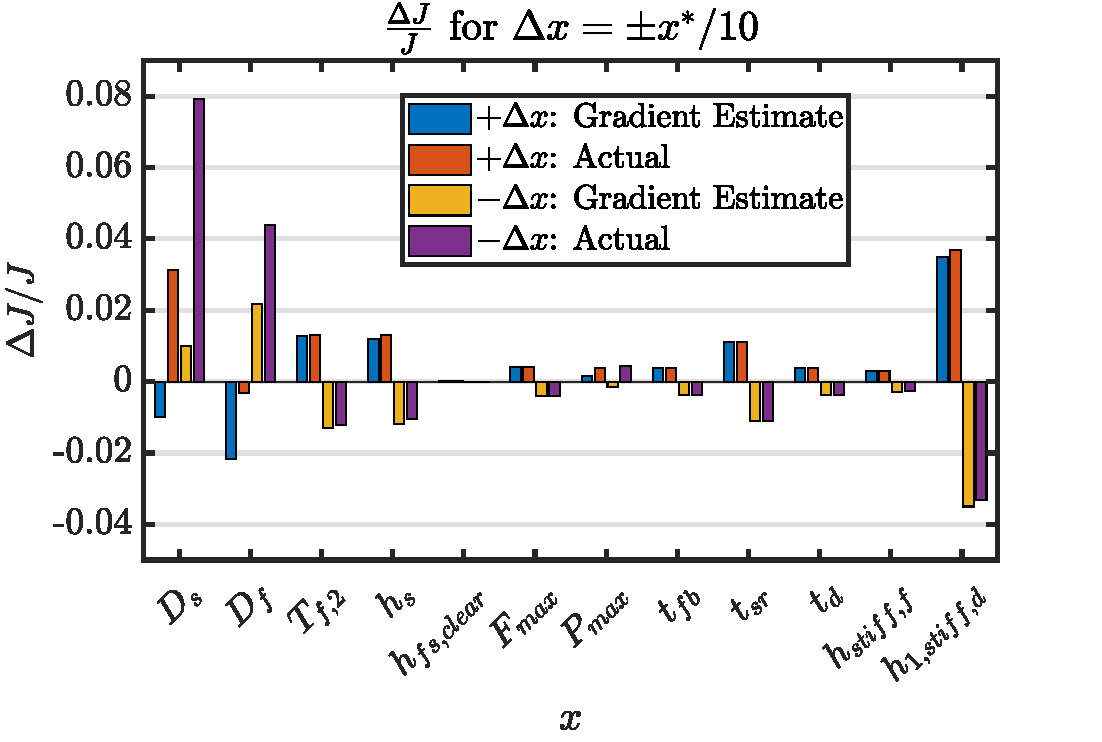
\includegraphics[width=\linewidth]{figs/delta_x.pdf}
\caption{Change in objective for perturbation of design variables from the minimum LCOE design}\label{fig:delta-J}
\end{figure}

The design variables with the highest sensitivities are $D_s$, $D_f$,and $h_{stiff,f}$, with a 10\% decrease in the diameters and 10\% increase in the stiffener height leading to a 7.9\%, 4.4\%, and 3.7\% increase in LCOE respectively.
The remaining design variables have a notably low sensitivity, meaning that they can be perturbed from their optimal value by 10\% in either direction without affecting the objective by more than 1-2\% (although they may affect constraints).
Finally, the gradient estimates are generally accurate, with the exception of the diameters $D_s$ and $D_f$ and the peak power $P_{max}$.
For these variables, nonlinearity or curvature exists in the objective function, indicating a tradeoff in the objective that would produce an optimum even without any active constraints.
For the case of LCOE minimization, this is expected because increasing the diameters and power rating both increase the power production while simultaneously increasing the capital cost.
More accurate estimates of the perturbed LCOE can be obtained by using the Hessian of the objective to account for curvature, but this would need to be obtained via manual finite differences because the solver only returns the Hessian of the Lagrangian.

\subsubsection{Multi-Start}
Separately, because non-convex optimization can get stuck in a local minimum, 1000 random initial guesses are tested, although 974 are linear infeasible and discarded.
Of the 26 linear feasible starting points, none converge while meeting the Karush-Kuhn-Tucker (KKT) conditions for first-order optimality.
For the LCOE-minimization, 17 optimizations converge due to small steps in the design while 9 fail to converge, and for the design cost minimization, that split is reversed, 9 and 17.
Of the optimizations that converge, 5 and 4 from the LCOE and design cost minimization respectively converge to the same minimum, referred to here as the global minimum since it is the lowest objective obtained across all starting points, although global optimality is never guaranteed.
On the other hand, more points (12 and 5 respectively) converge to a less optimal local minimum.
Of the optimizations that fail to converge, only one arrives at the same global minimum in each case.
\figureautorefname~\ref{fig:multistart-tree} shows this behavior on a probability tree.
Overall, around one fifth of the optimizations converge to the presumed global minimum.
Therefore, for a 95\% chance of obtaining the global optimum, a multi-start with at least $\textrm{ceil}\left(\frac{\ln(1-0.95)}{\ln(1-0.2)}\right)=\numMultistartRequired$ linear feasible starting points is required.
%\hl{XX}\% converged to the same point as the initial optimization did and none converged to a more optimal solution. While this does not guarantee a global optimum, the insensitivity to initial guess increases our confidence in the optimization results. 
\hl{Note to scrutineers: due to the high amount of linear infeasibility, I am going to try this again but generate points that are linear feasible from the start.}

\begin{figure}
\centering
\includegraphics[width=1.2\linewidth]{\matlabFilepath{15.6_3}}
\caption{Probability tree for convergence of multi-start}\label{fig:multistart-tree}
\end{figure}

It is also worth investigating which characteristics of the starting point contribute to the outcome of the optimization. 
\figureautorefname~\ref{fig:multistart-bar} shows a bar chart of the convergence behavior as a function of the starting point for each design variable.
It shows that the float draft $T_{f,2}$ and float bottom plate thickness $t_{f,b}$ usually converge to the same optimal $\vec{x}^*$ value regardless of the starting point $\vec{x_0}$, but the other design variables are very sensitive to starting point.
This sheds light on the convexity of the search space, indicating that the float draft and bottom plate thickness are close to unimodal, while the other design variables are highly multimodal.

\begin{figure}
\centering
\includegraphics[width=\linewidth]{example-image-a}
\caption{Bar chart showing impact of starting point on convergence behavior}\label{fig:multistart-bar}
\end{figure}

Future studies can use this knowledge to potentially reduce the total number of function evaluations required to achieve the global optimum.
For example, to reduce the number of iterations within each optimization, the multistart procedure could use deterministic starting points for the float draft and bottom plate thickness, since sampling is necessary only for the multimodal design variables.
Meanwhile, the number of optimizations could be reduced by sampling multimodal variables from a non-uniform distribution to capture both multiple local minima.
More complete multistart results are shown in \appendixautorefname~\ref{sec:appendix-supplemental-results}.

% \begin{table}
% \begin{tabular}{c|c|c}
%    Objective & Cost & Power \\ \hline
%    Converged to any solution & XX & XX \\
%    Converged to same optimum & XX & XX \\
%    Converged to better optimum & 0 & 0 \\
% \end{tabular}
% \caption{Sensitivity to starting point}
% \end{table}

\subsection{Single Objective Sensitivity Analysis}\label{sec:sensitivities}
\subsubsection{Local Sensitivity to Parameters}\label{sec:sensitivities-local}
It is useful to start with local parameter sensitivity results.
The present section focuses on interpreting the results of the most accurate local sensitivty method: perturbing each parameter a small amount from its nominal value and repeating the optimization, while \appendixautorefname~\ref{sec:appendix-sensitivties} compares the accuracy and computation time of multiple computation methods.
The re-optimization accounts for nonlinearities and is thus more accurate but requires significantly more computation time to obtain than local sensitivities obtained with post-optimality derivatives.

\figureautorefname~\ref{fig:param-sens-J-star-tornado}, \ref{fig:param-sens-x-star-tornado}, and \ref{fig:param-sens-x-star-tornado-2} show Tornado charts for the parameters with highest normalized sensitivities for the objective and design respectively.
Results are normalized such that a value of 1 means that a given percent increase in the parameter from its nominal value causes the same percent increase in  $J^*$ or $x^*$.
\begin{figure}
    \centering
    \includegraphics[width=1\linewidth]{\matlabFilepath{16}}
    \caption{Tornado chart showing highest objective sensitivities}
    \label{fig:param-sens-J-star-tornado}
\end{figure}

Analyzing the left side of \figureautorefname~\ref{fig:param-sens-J-star-tornado}, the value of the minimum LCOE is highly sensitive to the operational wave characteristics, with normalized sensitivities of $-1.4$.
This means that a 1\% increase in wave height or period leads to a 1.4\% decrease in LCOE due to increased power production.
Meanwhile, the LCOE is also sensitive to array availability and transmission efficiency (normalized sensitivity $-1.0$) and PTO efficiency (normalized sensitivity $-0.8$).
The 1:1 correspondence for array efficiency is expected since it directly multiplies the annual energy production, as is the slightly lower value for PTO efficiency since it multiplies energy only in the sea states which are not at the power limit.
Another high sensitivity is the fixed charge rate ($FCR$), at a value of $+0.84$.
While modeled as constant in MDOcean, the $FCR$ itself scales positively with the interest rate (normalized sensitivity $+0.21$) and negatively with device lifetime (normalized sensitivity $-0.45$).
This puts the normalized sensitivity of LCOE to interest rate and lifetime at $+0.18$ and $-0.38$ respectively.

Moving to the right side of \figureautorefname~\ref{fig:param-sens-J-star-tornado}, overall the sensitivities are higher: the minimum LCOE has 5 parameters with normalized sensitivity magnitude above 0.5, whereas the minimum design cost has sixteen such parameters.
The minimum design cost is most sensitive (normalized value $+2.1$) to the nondimensional damping plate stiffener height $h_{stiff,d}/h_{1,stiff,d}$, indicating that future optimizations should consider adding this as a design variable.
Other high sensitivities including $D_d/D_s$ ($+1.7$), $D_{d,tu}$ ($-1.6$), $D_{d,min}$ ($-1.1$), and $w_{stiff,d}/h_{1,stiff,d}$ ($-1.0$) also relate to the damping plate geometry and no float or spar geometric parameters have high sensitivity, indicating that the damping plate design drives the minimum achievable cost.
This begs the question whether it is worth having the damping plate at all, or if WECs with a low power, low cost design objective would do better to remove the need for a damping plate by fixing the spar to the sea floor, if the water is sufficiently shallow to do so.
This comparison is worth quantifying in future optimization studies. 

Meanwhile, the price of power $\$/W$ also has a high normalized sensitivity ($-2.1$), though notably the price of force $\$/N$ has too low a sensitivity to appear on the chart.
Site parameters ($h$, $-1.8$; $H_s$, $-1.6$; $T_{struct}$, $+1.4$; and $H_{s,struct}$, $+1.1$) also have high sensitivities, though interestingly the sign of the sensitivity for $T_{struct}$ has changed compared to the minimum LCOE point, such that a larger structural period decreases the minimum LCOE but increases the minimum design cost.
Based on the $N_{WEC}$ sensitivity, adding an additional WEC to the 100-WEC array will decrease the minimum per-WEC design cost by $1.1\%$ due to the economies of scale built into the economic model, an effect not observed in the LCOE minimization.
Unintuitively, the sensitivity to the material yield strength is positive ($+1.0$), such that a stronger material results in a more expensive design.
This is because with several structural thicknesses at their lower bound, the structural cost cannot be significantly reduced, and instead the added strength is leveraged by moving to a more expensive design with larger bulk dimensions and higher loads. %\hl{(This still doesn't make sense, the larger bulk design would only be chosen over the baseline design if it made the cost lower, since power is the held the same as a constraint for the min-cost optimization).}
Finally, the minimum design cost is sensitive to material density and cost (both $+0.6$).
This indicates the potential desirability of a lighter, cheaper material for the low power WEC.
The two sensitivities are expected to be equal due to the mass-based material cost model.

\begin{landscape}
\begin{figure}
    \centering
    \includegraphics[width=1\linewidth]{\matlabFilepath{17}}

    \caption{Tornado chart showing highest design variable sensitivities at minimum LCOE}
    \label{fig:param-sens-x-star-tornado}
\fillandplacepagenumber
\end{figure}
\end{landscape}
\begin{landscape}
\begin{figure}
    \centering
    \includegraphics[width=1\linewidth]{\matlabFilepath{18}}
    \caption{Tornado chart showing highest design variable sensitivities at minimum design cost}
    \label{fig:param-sens-x-star-tornado-2}
\fillandplacepagenumber
\end{figure}

 \end{landscape}
%Figure~\ref{fig:constraint-sens} gives the estimated parameter change threshold required to make inactive constraints active and active constraints inactive. Values are again normalized, where here a value of 1 means that a parameter would need to double (increase by 100\%) before the constraint activity changes.

Meanwhile, \figureautorefname~\ref{fig:param-sens-x-star-tornado} depicts sensitivity of optimal design variables to parameters, $\frac{d\vec{x}^*}{d\vec{p}}$. 
Unlike the objective sensitivities, which describe the effect of parameter changes on WEC viability, the design variable sensitivities describe the effect of parameter changes on the optimal design. 
For parameters representing uncontrollable external inputs, such as many site parameters, high values indicate a need for certainty of the parameter value early in the design cycle to ensure that the ultimate design is appropriate for the real parameter values.
For parameters representing controllable design choices that were held fixed rather than optimized for the sake of simplicity, such as many geometric parameters, high values indicate that future studies should include the value as a design variable instead of a parameter.

The design variable values which minimize LCOE are most sensitive to site (black) and geometric (red) parameters, with a subset of structural design variables ($t_{sr}$, $h_{stiff,f}$, and $h_{1,stiff,d}$) also being sensitive to structural (yellow) parameters.
In \figureautorefname~\ref{fig:param-sens-x-star-tornado-2}, the design variables which minimize design cost are sensitive to these three parameter categories plus economic parameters.
Dynamic parameters (blue), including the float and spar drag coefficients and PTO efficiency, do not significantly affect the optimal design in either case.
The low sensitivity to the drag coefficients in particular is notable because it means that it is likely not necessary to expend additional model development effort to capture the variation in drag coefficient with hull shape, wave frequency, material surface roughness, or other quantities.
It is also apparent that some of the structural thicknesses ($t_{fb}$ and $t_d$ in both optimizations, and $t_{sr}$ in the design cost minimization) are insensitive to all parameters because the optimal value is consistently at the lower bound.
This reinforces the aforementioned need for future enhancements to the structures model to better capture local buckling behavior for thin-skinned stiffened shells.

Looking at geometric parameters more specifically to assess if any should become design variables, we observe that $D_d/D_s$ strongly (normalized value above 0.5) affects the optimal values of four design variables ($D_s$, $t_sr$, $h_s$, and $h_{stiff,f}$), indicating that $D_d$ should be a design variable in future optimizations to ensure the coupling is adequately captured.
The parameter driving the float draft slant angle, $T_{f,1}/T_{f,2}$, has a high effect on the overall draft $T_{f,2}$, indicating that $T_{f,1}$ should also be a design variable.
The parameter driving the spar slenderness, $T_s/D_s$, significantly affects the spar height and float spar clearance $h_s$ and $h_{fs,clear}$, indicating that $T_s$ should be added as a design variable in addition to $h_s$.
Finally, the amount of clearance between the float and spar, $D_{f,in}/D_s$, has a large effect on  $h_{stiff,f}$.
This might suggest the addition of $D_{f,in}$ as a design variable, but a more significant gap between the float and spar would change the hydrodynamics in a way that is not modeled due to moonpool resonance effects, making this addition less straightforward than others. 
%\hl{Any other params that could have been design variables, show that the sensitivity is hopefully low.}
In summary, the parameters that should be added as design variables in future optimizations are $D_d$, $T_{f,1}$, $T_s$, and possibly $D_{f,in}$.

%Highly sensitive parameters include \hl{XXX}.
%Insensitive parameters include \hl{XXX.
%Describe which are sensitive to J vs x vs constraint activity.
%Maybe also show dJ/dx and that's important because you need that DV exact or not without affecting your bottom line.}
%\hl{Is it possible to use these sensitivities to demonstrate coupling, and predict the effect of holding some DVs constant?) - during re scrutineering} 

%For these highly sensitive parameters, it is worthwhile to perform a global sensitivity analysis to observe any nonlinearity. Figure~\ref{fig:param-sens-global} and \ref{fig:x-opt-sens-global} demonstrate the new optimal objective and optimal design variable values respectively under the re-optimization-based OAT global parameter sensitivity process described in section~\ref{sec:single-obj-process}.
% \begin{figure}\label{fig:param-sens-global}
% \includegraphics[width=\linewidth]{example-image-a}
% \caption{Global OAT parameter sensitivity analysis to optimal objective $J^*$}
% \end{figure}
% \begin{figure}\label{fig:x-opt-sens-global}
% \includegraphics{example-image-a}
% \caption{Global OAT parameter sensitivity analysis to optimal design $x^*$}
% \end{figure}

%The global sensitivity analysis indicates that \hl{list parameters} have strongly nonlinear sensitivities over the range of interest. During re-scrutineering. \hl{Sentence interpreting any params that aren't location based}. 

\subsubsection{Global Sensitivity to Deployment Location}
The high sensitivity to wave conditions warrants further analysis.
An additional global sensitivity analysis is conducted by reoptimizing for several discrete deployment locations.
This captures any interactions between the simultaneous changes to wave height, wave period, water depth, and storm sea state which previous local sensitivity analysis cannot capture due to its OAT nature.
Additionally, it shows the effect of different bandwidth seas, or the tendency for energy to be concentrated in one frequency or spread out across the spectrum, which is not captured in the previous results.
This will reveal not only which locations are most favorable for WEC deployment through the resulting LCOE, but also whether the optimal WEC design is robust to location through the resulting optimal design variables.
The effect of wave conditions on design is especially important considering that global deployability is a core requirement for WEC viability \cite{bull_systems_2017} and the ability to use a single WEC design across different wave conditions facilitates economies of scale and design convergence.

Wave resource data for four U.S. locations (Humboldt Bay, California; Pac-Wave North, Oregon; Pac-Wave South, Oregon; and Wave Energy Test Site, Hawaii) is obtained from the NREL SAM repository \cite{janzou_sam_2022}, which sources its data from a 2015 report by Sandia National Lab \cite{dallman_characterization_2015}.
All economic assumptions are held fixed for consistency, which neglects the effect of location-specific bathymetry on foundation cost and distance from shore on installation, operations, and maintenance costs.
The optimal design variables and LCOE corresponding to each of the four locations are shown in Table~\ref{tab:location}.

\begin{table}\label{tab:location}\setlength\arraycolsep{1pt}
\begin{tabular}{>{\centering\arraybackslash}p{0.22\linewidth}>{\centering\arraybackslash}p{0.08\linewidth}>{\centering\arraybackslash}p{0.17\linewidth}>{\centering\arraybackslash}p{0.17\linewidth}>{\centering\arraybackslash}p{0.17\linewidth}>{\centering\arraybackslash}p{0.18\linewidth}}
&& \multicolumn{4}{c}{Location}\\  \cline{3-6} 
& Symbol & Humboldt, CA & PacWave North, OR & PacWave South, OR & Wave Energy Test Site, HI\\ 
\hline 
Most frequent wave & - & $H_s = 1.25$m, $T_e=7.5$s & $H_s = 1.25$m, $T_e=8.5$s & $H_s = 1.75$m, $T_e=8.5$s & $H_s = 1.75$m, $T_e=6.5$s \\ 
Incident energy flux (kW/m) & $J$ & $32.2 $ & $37 $ & $40.7 $ & $14.3 $ \\ 
Half-power bandwidth (rad/s) & $BW$ & $390 \cdot 10^{-3}$ & $250 \cdot 10^{-3}$ & $240 \cdot 10^{-3}$ & $370 \cdot 10^{-3}$ \\ 
%Storm sea states (m, s) & $H_{s,storm},T_{e,storm}$ &  &  &  &  \\ 
Water depth (m) & $h$ & $45 $ & $50 $ & $65 $ & $55 $ \\ 
Opt. spar diameter & $D_s^*$ & $6 $ & $6 $ & $6 $ & $6 $ \\ 
Opt. float diameter & $D_f^*$ & $27.9 $ & $25.1 $ & $26.9 $ & $37.3 $ \\ 
Opt. float draft & $T_{f,2}^*$ & $990 \cdot 10^{-3}$ & $990 \cdot 10^{-3}$ & $990 \cdot 10^{-3}$ & $4.31 $ \\ 
Opt. spar height & $h_s^*$ & $38.4 $ & $38.6 $ & $39.7 $ & $39.5 $ \\ 
Opt. float-spar clearance height & $h_{fs,clear}^*$ & $3.9 $ & $3.93 $ & $3.99 $ & $1.8 $ \\ 
Opt. maximum force & $F_{max}^*$ & $2.44 $ & $3.36 $ & $6.61 $ & $2.98 $ \\ 
Opt. maximum power & $P_{max}^*$ & $286 $ & $286 $ & $286 $ & $288 $ \\ 
Opt. float bottom thickness & $t_{fb}^*$ & $13.4 $ & $13.7 $ & $14.2 $ & $1.27 $ \\ 
Opt. spar radial thickness & $t_{sr}^*$ & $25 $ & $25.1 $ & $25.4 $ & $7.21 $ \\ 
Opt. damping plate thickness & $t_d^*$ & $25 $ & $25.2 $ & $25.4 $ & $1.31 $ \\ 
Opt. float stiffener height & $h_{stiff,f}^*$ & $170 \cdot 10^{-3}$ & $196 \cdot 10^{-3}$ & $249 \cdot 10^{-3}$ & $261 \cdot 10^{-3}$ \\ 
Opt. damping plate stiffener height & $h_{1,stiff,d}^*$ & $389 \cdot 10^{-3}$ & $423 \cdot 10^{-3}$ & $585 \cdot 10^{-3}$ & $956 \cdot 10^{-3}$ \\ 
Opt. levelized cost of energy (\$/kWh) & $LCOE^*$ & $605 \cdot 10^{-3}$ & $605 \cdot 10^{-3}$ & $539 \cdot 10^{-3}$ & $513 \cdot 10^{-3}$ \\ 
\end{tabular}
\caption{Results for Re-Optimization in Four Distinct Locations}
\end{table}

All optimized LCOE values are less expensive than the RM3 baseline.
The WEC located in Pac-Wave South, OR results in the lowest LCOE, \$\LCOEPacWaveNorth/kWh, which makes sense because the incident wave energy flux is highest there.
The WEC located in WETS, HI has the highest LCOE, \$\LCOEHawaii/kWh, aligning with its low incident energy.
The values of the optimal design are similar for the California and Oregon locations, but quite different for Hawaii, with the latter having a \HawaiiDesignCharacteristics.
This is surprising: using the simple scaling argument $\omega_n = \sqrt{\frac{k}{m}}=\sqrt{\frac{\rho g A}{\rho A T_f C_m}}\sim T_f^{-\frac{1}{2}}$ a WEC's uncontrolled natural frequency scales with its draft to the $\frac{-1}{2}$ power, so a smaller draft would be expected in sites with higher-frequency waves like Hawaii.
One hypothesis for this reversal is that Hawaii's lower incident energy and thus lower wave excitation force requires a higher oscillation amplitude to achieve comparable energy production, which in turn necessitates a higher draft to avoid slamming.
\hl{(I'm not sure if this is the true explanation, need to inspect intermediate results to confirm.)}
This result demonstrates the importance of using a full coupled model to optimize WEC design, as the simple scaling heuristic produces an inaccurate conclusion.
\hl{(Note: I may replace one of the PacWaves with North Carolina so I have a result from the East coast.
I would also like to include the results of holding design constant, ie with each output row having another row below it showing the ratio from using} $x^*_{California}$ at that location).

%\subsubsection{Price Global Sensitivity}
%We also perform a global sensitivity analysis for price parameters $p_\tau$, $p_P$, $p_M$, and $p_0$ from equation~\eqref{eq:LCOE-scale}. For $p_0$, if the design-independent (unmodeled) cost goes to zero, \hl{(and maybe change 80\% efficiency into 100\%)}, that's essentially the best LCOE that a WEC of these technical assumptions (steel point absorber with given operational conditions) can get. We can think of the rest as a cost gap \hl{(explain)}. Meanwhile, the global sensitivity analysis for $p_\tau$ gives preliminary insight into the multi-objective problem, recovering a portion of the pareto front between the four variables that influence $LCOE$: $\tau$, $P_{pk,elec}$, $V_{struct}$, and $P_{avg,elec}$. This shows \hl{XXX conclusion}, to be clarified further in the multi-objective optimization.

\subsubsection{Global Sensitivity to Modeling Assumptions}
\label{sec:sensitivity-model-assumptions}
In addition to continuous parameters, the simulation depends on discrete options that dictate model behavior.
These settings include the control scheme (damping or reactive), the presence of generator force saturation, the presence of drag, and the number of dynamic degrees of freedom (float heave motion only or float and spar heave motion).

\paragraph{Control Scheme}
\hl{This analysis is left for during scrutineering.}

\paragraph{Force Saturation}
First examining the optimal LCOE design presented in \sectionautorefname~\ref{sec:results-single}, the lowest force saturation power factor across all sea states in \figureautorefname~\ref{fig:power-matrix-opt} is $\frac{P_{sat}}{P_{unsat}}=\lowestFmaxFactorMinLCOE$, with a corresponding force limit of $\frac{F_{max}}{F_{unsat}}=\lowestFsatMinLCOE$~in that sea state. 
%This corresponds almost exactly with the relationship expected in the purely resistive Thevenin impedance case in \cite{mccabe_force-limited_2024}:
%\begin{equation}
%   \frac{ P_{sat}}{P_{unsat}}=1-\left(\frac{F_{max}}{F_{unsat}}-1\right)^2
%\end{equation}
% see notebook p46 5/16/25
% fixme: what about the factor of 4/pi in the force ratio? Then the quadratic equation wouldn't apply, it would be more complicated (alpha non zero case) which casts doubt on my conclusion that alpha=0 emerges as optimal. Would need to compute alpha directly I think? I also think that the assumption of damping control means my Im(Gamma)=0 assumption in the notebook is false. Also Psat/Punsat is the the same as Psat/Pmax. So leaving this sentence out.
Considering all sea states, the optimal force-saturated design sacrifices only \powerLossForceSatMinLCOE~Watts of average power (around \pctPowerLossForceSatMinLCOE) and reduces its PTO cost by \pctPTOSavingsForceSatMinLCOE, leading to an LCOE reduction of \pctImproveLCOEForceSatMinLCOE~compared to the same design with no force saturation, although the unsaturated design violates structural constraints due to the higher force.
If the optimization is instead re-run to ensure constraint satisfaction while not allowing force saturation, the result has a \pctPowerLossForceSatOptMinLCOE~power gain, \pctPTOSavingsForceSatOptMinLCOE~higher PTO cost, \pctStructSavingsForceSatOptMinLCOE~higher structural cost, and \pctImproveLCOEForceSatOptMinLCOE~higher LCOE compared to the optimization with saturation.

\paragraph{Drag}
As section~\ref{sec:sensitivities-local} alludes to, the low sensitivity to drag coefficient suggests that modeling the drag nonlinearity is perhaps not essential.
This is surprising, because without drag the resonant amplitude is significantly higher, which should affect the results due to the active slamming constraint.
One reason for this discrepancy is that the drag sensitivity was local only, and a re-optimization at $C_d=0$ would likely yield different results.
\hl{Performing this re-optimization is left for during scrutineering.}

\paragraph{Degrees of Freedom}
\hl{This analysis is left for during scrutineering.}

\clearpage
\subsection{Multi-Objective Optimization}\label{sec:results-multi}
In the multi-objective optimization, the design-dependent capital cost $C_{design}$ and the average electrical power $P_{avg,elec}$ are optimized simultaneously to show the trade-off between the two quantities.
As described in section~\ref{sec:multi-obj-process}, the multi-objective analysis gives important insights for cases where the LCOE may not apply or is uncertain due to variation in cost variables modeled as constant, including $OPEX$, $FCR$, and $p_0$.
A pareto front is shown in Figure \ref{fig:pareto}, with the utopia point marked with a green star, simulated designs marked with squares, and the actual performance of the nominal design as reported in \cite{RM3} marked with a diamond.
All designs on the Pareto front have a significantly lower cost than the nominal RM3 design, with a range of powers both smaller and larger than the nominal.
Figure~\ref{fig:pareto-lcoe} provides a zoomed-in version with superimposed contours of constant $LCOE$ for reference.
The minimum LCOE design occurs at the point of tangency between the pareto front and the LCOE contours and very nearly coincides with the maximum power design. %\hl{analyze more: how are the max power and min LCOE designs different? talk about the multiple apparent points of tangency (ie at 50 cents/kWh) and whether those are local minimums in LCOE.}
\begin{figure}
    \centering
    \includegraphics[width=.8\linewidth]{\matlabFilepath{19}}
    \caption{Pareto Front}
    \label{fig:pareto}
\end{figure}
\begin{figure}
\centering
\includegraphics[width=.8\linewidth]{\matlabFilepath{20}}
\caption{Pareto front with different LCOE contours overlaid }
\label{fig:pareto-lcoe}
\end{figure}

There exists a cusp in the pareto front at the point where the average electrical power is around \powerWhereCusp~kW.
As a result of this cusp, the bulk of the pareto front (extending from the least-cost design at \powerAvgAtMinCapex~kW to around \powerWhereNonconvexEnds~kW) is non-convex.
This region would have been missed with a convex multi-objective optimization procedure that optimizes weighted sums of the objectives, affirming the necessity of the epsilon-constraint plus pattern search procedure used here.

Figure~\ref{fig:pareto} inlays geometry visualizations for a few designs highlighted in light blue.
One apparent trend is that the optimal spar draft and float diameter increase in size as one moves from left to right along the Pareto front.
This makes sense intuitively: to minimize material, the components will be as small as possible while satisfying constraints.
Larger dimensions incur higher costs and allow more power generation.

Similar trends are explored more quantitatively in Figure \ref{fig:design-heuristics}.
The graph provides extremely useful design heuristics for how to adapt WEC design to a given application, depending on the desired balance between cost and power output.
In the interest of showing consistent, easily interpretable trends even with random, non-uniform spacing of points, the x-axis shows the percent along the pareto front, calculated by scaling the angle of each pareto point from the nadir point, and the y-axis values are lightly smoothed with a low pass filter.
To facilitate comparison against the pareto front in Figure~\ref{fig:pareto} and visualize clusters, the individual pareto points are shown as black squares on the x-axis of Figure \ref{fig:design-heuristics}.
Structural design variables are green, powertrain ratings are blue, and bulk geometry dimensions are red. 
\begin{figure}
    \centering
    \includegraphics[width=1\linewidth]{\matlabFilepath{21}}
    \caption{Design and objective heuristics plot}
    \label{fig:design-heuristics}
\end{figure}

Analysis starts by examining the direction of the changes.
With increasing cost and increasing average power (from left to right in the figure), most design variables either monotonically increase ($P_{max}$, $D_s$, and $t_{s,r}$) or almost monotonically increase with one brief decline ($F_{max}$, $D_f$, $h_{1,stiff,d}$, and $h_s$).
Just two design variables are mainly decreasing: $T_{f,2}$ and $h_{fs,clear}$, both variables involved in the float amplitude constraints.
Two of the remaining three design variables ($t_d$ and $t_{f,b}$, structural thicknesses at their lower bound) stay constant across the pareto front with the exception of a few small upwards excursions in $t_d$ around 2\%, 23\%, and 60\% of the way through, while the final variable $h_{stiff,f}$ experiences several small oscillations. 

Analyzing the magnitude of changes, the powertrain ratings differ the most drastically across the pareto front, while geometric and structural variables require only moderate adjustments.
This begs the question: how much are the cost savings at lower powers driven by the smaller PTO cost compared to the smaller material cost?
If PTO cost dominates the savings, WEC companies selling devices at multiple power levels may want to maintain the same geometric and structural design across all products, changing only the PTO, which reduces design effort and facilitates economies of scale compared to changing all subsystems.
Using the cost values in the earlier Table~\ref{tab:opt-dv-values}, unfortunately only \pctCostSavingsFromPTO~of the cost savings come from the smaller PTO, indicating that for a lower power WEC under the previously stated price assumptions, the slightly smaller hydrodynamic design is actually much more important to pursue than the substantially smaller PTO.
Therefore, design reuse across varying power levels is unlikely.
This conclusion differs from preliminary work \cite{mccabe_multidisciplinary_2022} which wrongly examined only the change in the optimal design without taking into account the relative impact of PTO and device dimensions on cost.

Meanwhile, the bottom part of \figureautorefname~\ref{fig:design-heuristics} provides a similar insight on how values change across the pareto front for objectives instead of design variables. % change objectves to outputs - ie LCOE, CF, X_max, all the y* in single objective.
The power output is largely linear, while the design cost experiences a discrete change in slope at around 5\% and a gradual change beyond that.
The discrete slope change causes the aforementioned cusp in the pareto front, and the figure now elucidates that this corresponds to a change in PTO sizing strategy: from 0-5\% along, the cost-power tradeoff is achieved by adjusting the maximum power, whereas from 5-70\% along it is achieved by adjusting the maximum force while maintaining constant maximum power.
The gradual design cost slope change indicates diminishing returns (an increased marginal cost of additional power generation).

%An additional point of note on the Pareto front of Figure \ref{fig:pareto} is the LCOE and coefficient of variation of a typical solar array plotted for comparison (data from \cite{borettiSolar}). Even the cheapest WEC design is still almost an order of magnitude more expensive than solar, indicative of the immaturity of WEC technology and the need for further innovation and cost reduction. On the bright side, many of the designs achieve a lower coefficient of power variation than solar, indicating the potential for wave energy as a relatively steady grid-connected renewable. Finally, it is worth highlighting that the amount of power variation directly affects the required energy storage, so the local cost of storage affects the position along the Pareto front that is optimal for a given application.

%We can plot LCOE contours under different economic assumptions (sweep a couple FCRs, p0s, and opexes) and overlay this to the results already obtained in the global sensitivity analysis of FCR, p0, and opex but now plotted in multiobjective space.\hl{(Explain this better)}

Figure~\ref{fig:constraint-activity} shows which optimization constraints are active along the pareto front.
Three structural design variables ($t_d$, $h_{stiff,f}$, and $h_{1,stiff,d}$) hit their lower bound, while none hit their upper bound.
The only linear constraint active is the spar natural frequency constraint.
Since this constraint was marked as priority two (required for modeling accuracy given the assumptions), its activity is significant and will be discussed more in section~\ref{sec:discussion}.
Aside from the irrelevant maximum force constraint, which is always active by design, active nonlinear constraints include the float, column, and damping plate structural factors of safety, and the amplitude constraints preventing the float from rising above the spar, maintaining linear wave theory, and preventing slamming of the float.
\begin{figure}
    \centering
    \includegraphics[width=1\linewidth]{\matlabFilepath{22}}
    \caption{Constraint Activity}
    \label{fig:constraint-activity}
\end{figure}

%\hl{If there's room/time, consider a bonus pareto of LCOE vs CF.}

%\subsection{Multi-Objective Sensitivity Analysis}
%\hl{This section I don't have results for yet and can be cut if needed. Maybe show trace out the effect of parameter variation without reoptimizing in multiobjective space, and it shows you how far some param variations bring you from optimal, like the dJ/dp sensitivities before but now for everywhere on the pareto front, and visualized differently. Perhaps also do re-optimized pareto fronts for a parameter or two that was found to be highly influential in the single objective analysis. Also show the effect of keeping geometric DVs fixed and what the new pareto front and design heuristics curve would look like.}

\subsection{Optimization Runtime}
Figure \ref{fig:optim-runtimes} shows the runtime for each optimization and analysis routine, as run in parallel on the 14-core server described in section~\ref{sec:sim-runtime}. 
The optimization also runs without issue, albeit more slowly, on unspecialized machines such as a Windows 10 laptop computer with MATLAB R2022a.

\begin{figure}
\centering
\includegraphics[width=\linewidth]{\matlabFilepath{26}}
\caption{Bar chart of optimization and analysis runtimes}
\label{fig:optim-runtimes}
\end{figure}
%the standard GitHub Linux runner for public repositories, which has 4 CPUs and 16 GB RAM with Ubuntu 24.04 operating system.
Each single-objective optimization takes just \singleObjRuntime, converging in \singleObjIters~iterations and requiring \singleObjFcnEvals~function evaluations including both objective and gradient evaluation. 
Generating the pareto front takes \paretoRuntime, of which \paretoPctTimeSeeds~is spent generating seeds via epsilon-constraint and the remaining \paretoPctTimePatternSearch~on the pattern search. 
Gradient-based post-optimality sensitivities run rapidly in just \gradientSensRuntime, while sensitivities obtained via re-optimization take \reoptimSensRuntime.

\figurename~\ref{fig:pareto-epsilon-runtime-sweep} shows the effect of the number of epsilon-constraint seeds on the number of function evaluations and hypervolume. (\hl{Analysis is left for during scrutineering.})

\begin{figure}
\centering
\includegraphics[width=\linewidth]{example-image-a}
\caption{Effect of number of epsilon-constraint seeds on pareto front function evaluations and hypervolume}
\label{fig:pareto-epsilon-runtime-sweep}
\end{figure}

\clearpage
\section{Discussion}\label{sec:discussion}

Beyond the analysis of individual results offered in section~\ref{sec:results}, this section discusses the study's contributions, implications, and limitations more broadly.
It compares results to existing studies for context and suggests avenues for future work to resolve model shortcomings and answer additional design questions.

\subsection{Result Comparison to Other Studies }
% (and comparison to commercial WECs)
\subsubsection{Force Saturation}
Previous studies \cite{mcgilton_optimal_2024,coe_maybe_2021,devin_high-dimensional_2024,gaebele_tpl_2025,mccabe_force-limited_2024} suggest capping the maximum force significantly below the unsaturated point based on findings that doing so sacrifices only minimal power, but none perform full economic analysis to confirm that the cost savings outweigh the power decrease.
The results presented in section~\ref{sec:results-single} verify the conclusion with an appropriate cost analysis, since the optimal design sizes its powertrain small enough to necessitate force saturation.
The follow-on analysis in \sectionautorefname~\ref{sec:sensitivity-model-assumptions} repeats the optimization without allowing force saturation and finds a 5\% LCOE penalty.
Thus, force saturation as a control technique is highly valuable, capable of tangible LCOE reductions when considering the tradeoff of power and cost.
Future studies could quantify the threshold of the lowest marginal price of PTO force (\$/N) for which this conclusion still holds.

% \hl{add similar analysis for power saturation}

\subsubsection{Global Deployability}
A survey indicates that 40\% of WEC developers design their WEC to be deployment-site agnostic, so design for global deployability is of interest in industry \cite{trueworthy_wave_2020}.
A previous study \cite{de_andres_adaptability_2015} compares the global deployability across different wave climates of a uniform WEC design versus a tunable WEC design.
The study finds that tuning the resonant period to match the dominant ocean period by changing geometry increases the capture width ratio but decreases the more important power to mass ratio (an inverse proxy for LCOE), concluding that tuning is unfavorable because it requires expensive larger diameters.
Importantly, however, the devices have equal diameter and height, use only damping control, and are tuned to maximize power without regard for mass or cost.
In MDOcean, on the other hand, tuning can not only be accomplished by changing diameter and height independently, but also with reactive control.
Moreover, devices are tuned not to maximize power but to minimize LCOE.
The single-objective results in \tableautorefname~\ref{tab:opt-dv-values} and \ref{tab:opt-output} show agreement with the overall conclusion of \cite{de_andres_adaptability_2015} that power maximization does not align with LCOE minimization, but in the present study the additional cost of maximum power comes in the form of PTO cost rather than structural cost as it does in \cite{de_andres_adaptability_2015}.
Meanwhile, MDOcean's location global sensitivity (\tableautorefname~\ref{tab:location}) shows a significantly larger optimal float size in Hawaii, the location with the lowest value of the most common wave period.
This again departs from the results of \cite{de_andres_adaptability_2015}, which finds that small (4~m diameter) WECs optimize their LCOE proxy regardless of the dominant period at the location.
This demonstrates that the use of a more thorough multidisciplinary model like MDOcean is essential to draw accurate design conclusions.

\subsubsection{Structural Efficiency}
A previous study compares the structural mass per unit hull volume for marine structures including WECs and ship hulls, finding a value of $278.76 $~kg/m\textsuperscript{3} for steel structures \cite{roberts_bringing_2021}, with a 95\% confidence interval of $\pm280$ metric tons.
This trendline would predict the nominal float structural mass to be 72-632 metric tons and the minimum LCOE structural mass to be 1814-2374 metric tons.
MDOcean calculates structural masses of 213 and 80 metric tons respectively.
The nominal design lies within the confidence interval, but the optimized design lies far below it.
Even though the hull volume of the optimal design exceeds the hull volume of any data points used to create the fit, the large departure from existing data warrants concern.
In fact, the only data points with structural mass comparable to the optimized 80 ton float have a hull volume that is an order of magnitude lower than the optimized float, indicating that MDOcean may vastly underestimate the required thickness.
This requires further investigation and may be due to underestimation of loads in the dynamics module or overestimation of the factor of safety in the structures module.

% compare to the Sandia RM3 optimization results

\subsubsection{Optimization Procedure}
\label{sec:discussion-optimization}
Recalling the discussion of prior WEC optimization studies in section~\ref{sec:lit}, all prior large-scale ($\geq8$ design variables) WEC optimizations utilize the genetic algorithm, a population-based heuristic algorithm.
Based on the generation count and population sizes stated in references \cite{khanal_multi-objective_2024,garcia-teruel_reliability-based_2021,cotten_multi-objective_2022,abdulkadir_control_2024}, 12,000, 2,200, 6,100, and 2,400 function evaluations are required for convergence respectively.
The the present study is the first to perform large-scale WEC optimization with a gradient-based algorithm, which was expected to require fewer function evaluations to converge.
Generating the pareto seeds in this study, however, entails performing 20 single-objective optimizations at around 100 iterations each, using finite difference on the 12 design variables.
This requires an estimated $20\cdot100\cdot(12+1)=\paretoFcnEvals$ function evaluations, which dwarfs the function evaluations required by the genetic algorithm in other studies.
This result is surprising and can be attributed to the use of finite difference.
Despite the greater function evaluations, MDOcean's semi-analytical model means that the optimization likely runs faster than the other BEM-based optimizations, although the relevant papers do not include any runtime information that could verify or deny this claim.
Because of the fast runtime, effort was not invested to decrease the number of iterations, although moderate reductions should be possible by tuning convergence criteria, utilizing a gradient sparsity pattern to reduce the number of finite difference evaluations needed, and tuning the ratio of the number of seeds to the pattern search set size.
A more substantial decrease is possible by using automatic differentiation or the adjoint method to obtain derivatives.
These methods would make the number of function evaluations independent of the number of design variables, but they require more implementation effort.
For example, the adjoint method would additionally require constraint aggregation because of the large number of constraints, and automatic differentiation would require rewriting all functions in terms of elementary functions where possible and manually supplying gradients for unsupported functions such as Bessel functions in the hydrodynamics module.
Finally, even with the increased function evaluations, the gradient-based algorithm retains its advantage of providing certainty that the solution has converged to a local optimum, and with a systematic multistart, there is reasonable confidence that the solution is a global optimum, which is not the case in a heuristic optimization.

\subsection{Model Realism}
Circling back to the modeling assumptions introduced in section~\ref{sec:model}, one can now use the optimization and sensitivity results to determine whether the assumptions are reasonable.
We assess model complexities that MDOcean adequately captures to confirm whether those effects were worth including, as well as model shortcomings that MDOcean cannot adequately capture to examine whether those effects must be added in future versions.
Previous studies such as \cite{garcia-teruel_reliability-based_2021} have called for this kind of systematic model fidelity assessment to enhance designers' confidence on the most relevant effects and their impact on computation time.

\subsubsection{Observed Impact of Modeled Effects}
A few of the areas of developed model complexity, such as force saturation, slamming amplitude limits, and 2-DOF dynamics, stand out as contributing significantly to the final results, as seen in the constraint activity and difference in results obtained if 1-DOF dynamics corresponding to a stationary spar are used.
Section~\ref{sec:sensitivity-model-assumptions} analyzed these effects in detail.
Earlier in \sectionautorefname~\ref{sec:sim-runtime}, \figureautorefname~\ref{fig:runtime-dynamics} reveals that MDOcean's 2-DOF dynamics take an order of magnitude longer to run than 1-DOF dynamics, indicating an area where code enhancements to make the 2-DOF runtime more comparable with the 1-DOF model may be worthwhile given the dynamic importance of including the second degree of freedom. 
Meanwhile, force saturation is seen to be especially relevant since it not only directly reduces the powertrain cost, but also indirectly reduces the structural cost by reducing the operational heave loading.
This allows for a reduction in spar thickness due to the activity of the column fatigue factor of safety constraint. 
The observed impact of these effects on the overall optimization justifies the model complexity in those areas, suggesting that other optimization frameworks should include these complexities for realistic results.

On the other hand, a few other modeling complexities appear perhaps unnecessary in hindsight because they have little effect on the results.
Section~\ref{sec:sensitivities-local} finds a low sensitivity to drag coefficient, and the re-optimization without drag in \sectionautorefname~\ref{sec:sensitivity-model-assumptions} confirms this result.%\hl{confirms this result}.
This suggests that modeling the drag nonlinearity is not essential, and future optimizations may wish to turn off drag to reduce the computation time associated with iterating the drag damping coefficient.
Likewise, the slamming model is derived to be valid not just in the simple case of long waves but also in intermediate wavelengths, where the maximum amplitude depends on additional values including the phase of the dynamic response.
\appendixautorefname~\ref{sec:appendix-slam} shows that the simple slamming model is reasonably accurate at sea states with active slamming constraint, suggesting that the intermediate wavelength model may be unnecessary.
However, before making this claim confidently, it would be necessary to check whether this is true at all points during the optimization, not merely at the optimal point, because the slamming model complexity is not currently implemented as a model setting and the suitability of the long-wave condition at the optimum is checked manually. %\hl{I should actually check this.}
Finally, even though it is observed that the drag and intermediate wavelength slamming models have little effect on the results individually, the nonlinearity of the problem permits the possibility that a coupling effect may be observed if both were to be turned off simultaneously, or that an effect may emerge if the formulation were to change in another way such as optimizing another objective or adding more constraints.
Therefore, users should exercise caution if choosing to simplify the model.

\subsubsection{Potential Impact of Unmodeled Effects}
No constraints corresponding to priority 1 or 2 requirements are active in the optimal solution, % \hl{(double check this - structures effective breadth could make this false)}, 
a hopeful sign that the true optimum is unlikely to lie in a region of model inaccuracy.
Likewise, the inactivity of the pitch stability constraint mitigates the impact of any error in the metacentric height due to the geometry module's assumption of an even mass distribution when calculating the center of gravity (see section~\ref{sec:geom}).
On the other hand, the active slamming constraints for operational sea states mean that some assumptions are worth revisiting, particularly the use of an optimization constraint rather than enforcing amplitude limits with the constrained optimal linear controller (see tables \ref{tab:constraint-approaches} and \ref{tab:nonlinearities}), and the assumption that the WEC must operate in all sea states with nonzero probability in the JPD without going into survival mode (see ``Dynamic Limits and Design Load Cases'' in section~\ref{sec:dynamics}).

\subsection{Formulation Realism}
\subsubsection{Design Variable Suitability}
Section~\ref{sec:formulation} outlined this study's careful choice of design variables to facilitate satisfaction of high-priority requirements to maintain model validity and facilitate optimization convergence while balancing the computational challenges of a large design space.
The analysis in \sectionautorefname~\ref{sec:sensitivities-local} reveals that the following variables chosen as parameters may be worthy of including as design variables in future studies: $D_d$, $T_{f,1}$, $T_s$, and possibly $D_{f,in}$.
In addition, the addition of $N_{WEC}$ as a design variable carries little importance in an LCOE minimization, where larger $N_{WEC}$ should always be preferred due to economies of scale, but can offer especially useful insight in a modified multi-objective analysis where the first objective is changed from per-WEC average power to array average power.
This is relevant for small-scale Powering the Blue Economy applications with a fixed power requirement, where it is unclear whether it preferable to meet that requirement using multiple smaller WECs or one larger WEC.

Additionally, a sensitivity analysis of design variables perturbed as if they are parameters would help to analyze the extent of coupling between disciplines and potentially inform future formulation simplifications.
For example, the expected high sensitivity of the optimal structural design variables to the powertrain design variables $\left(\frac{dx^*_{struct}}{dx_{pto}}\right)$ aligns with the choice made in this study to conduct fully coupled MDO, as outlined in section~\ref{sec:model-overview}, but a low value would support the potential disciplinary decoupling.
This type of analysis may be necessary if a proposed future optimization with significantly more design variables is too computationally intensive to perform fully coupled optimization and requires splitting up into a set of sequential optimizations, such as bulk geometry power maximization followed by powertrain sizing followed by structural sizing).
Performing this sequential optimization for the current formulation and assessing the degree of suboptimality could quantify the importance of a coupled optimization.
The authors predict, however, that the significant computational speedup of the semi-analytical models introduced in this paper and the extensions discussed herein will be sufficient to allow full coupling even for substantially larger scale WEC optimizations, including the ambitious target of a study comparing multiple hydrodynamic architectures with realistic powertrain models.

\subsubsection{Parameter Suitability}
The local parameter sensitivity analysis of \sectionautorefname~\ref{sec:sensitivities-local} already yields significant insight on the impact of the choice of parameters in this problem.
Interpreting those results more broadly, parameters with a high design sensitivity $\left(\frac{dx^*}{dp}\right)$, such as dimensional aspect ratios, wave conditions, and material properties, are especially important for engineers to determine early in the design cycle because they affect the optimal design. 
Where relevant, designers should consider holding the nondimensional versions of these parameters constant across prototype scales, extending the common practice of Froude scaling for wave conditions.
On the other hand, parameters with a high objective sensitivity $\left(\frac{dJ^*}{dp}\right)$, such as operational wave conditions, PTO efficiency, and financing rates in the LCOE minimization, are most important for funders to determine early in the project implementation cycle and for research funding agencies to incentivize innovation through R\&D proposals because they affect the WEC's economic viability.
Notably, other parameters such as PTO price, storm wave conditions, and dimensional variables are more relevant for design cost minimization, highlighting that incentives and innovation strategies for Powering the Blue Economy applications may need to be distinct from those for utility-scale energy.
Meanwhile, the larger number of parameters with high sensitivity in the cost minimization implies that there are more diverse avenues for impactful innovation in PBE applications than in utility-scale energy.

Additional sensitivity and post-optimality analysis work that could produce useful insights includes a sensitivity analysis of hyperparameters, following the same procedure as section~\ref{sec:sensitivities-local}, to ensure numerical convergence and adequate tuning of optimization settings.
A global parameter sensitivity analysis is also suggested, taking into account both nonlinearites in the effect of one parameter across operating points and interaction effects between multiple uncertain parameters.

\subsubsection{Constraint and Requirement Suitability}
By including \numLinConstraints~linear and \numNonlinConstraints~nonlinear constraints, this optimization captures more realistic design, model, and operational requirements than any other WEC optimization study known to the authors.
The active constraints highlighted in \figureautorefname~\ref{fig:constraint-activity} fall broadly into the class of survivability, including both structural (design variable lower bounds and factors of safety in each of the float, column, and damping plate) and amplitude-based (float rising above spar, linear theory, and float slamming). 
Constraints related to ballast and pitch stability are inactive, confirming that these design considerations are not primary avenues for innovation.
While survivability is known to be a critical design requirement for WECs, it is rarely incorporated into optimization studies, and the results of this study demonstrate and quantify the effect of survivability considerations. 
For example, the Lagrange multipliers of \figureautorefname~\ref{fig:lagrange-multiplier} suggest that improvements to the structural design of the damping plate are worth around 5 times more than equivalent structural improvements to the column and 10 times more than those to the float.

Further innovation in WEC survivability is warranted, both in the incremental and transformative sense.
Incremental improvements include developing more structurally and hydrodynamically performant detail designs that obey these constraints while reducing material use and sustaining energy production (for example, performing FEA or adding additional stiffeners to justify the removal of more material, replacing welded connections with pins to reduce moment transfer, or modifying the float-spar attachment geometry to allow for more travel with the same bulk body dimensions).
Transformative improvements include creative design concepts that avoid the need for these constraints altogether or substantially modify their formulation.
For example, storm survival strategies that involve submerging the WEC, changing the shape using control surfaces, or changing the PTO control strategy to reduce force and amplitude have all been suggested, and the viability of such design changes can be readily estimated by comparing the additional costs (for example, of additional actuator and control hardware and software) against the performance gains again using the Lagrange multipliers of \figureautorefname~\ref{fig:lagrange-multiplier}.

That said, there still exist many considerations that the formulation fails to capture, requiring caution before asserting that the industry should pursue the optimal design found here.
For one, design variables are assumed continuous, whereas in reality the sizing of structural thicknesses and, to a lesser extent, generator specifications, are constrained based on the discrete sizes available commercially.
Additional requirement omissions that could reasonably be considered in future work include mooring loads, structural resonant mode frequencies, and overturning moment in the storm design load case.
Requirements like installation and manufacturing feasibility, environmental and regulatory acceptability, reliability, and social benefit are more difficult to incorporate in the present modeling framework but nonetheless important.
For example, maximum dimensions may be limited by roadways, as is already the case for wind turbines, constraining maximum dimensions to 14-15 feet (4.3-4.6 m) \cite{cotrell_analysis_2014}.
Assessing the relationship between maximum component size (as transported) and maximum WEC dimensions (as installed) requires additional manufacturability and on-site assembly analysis beyond the scope of the present study.
To guide future work on requirements and constraints in WEC design optimization, the reader is referred to \cite{bull_systems_2017,babarit_stakeholder_2017} for a comprehensive breakdown and mapping of WEC requirements, and to \cite{trueworthy_wave_2020} for a study of how developers prioritize and address WEC design requirements in practice.

\subsubsection{Objective Suitability}
Due to the high uncertainty inherent in LCOE, this study performs multi-objective optimization on cost and power production and includes post-optimality analysis such as local and limited global sensitivity analysis.
While this overcomes many concerns in optimizing LCOE, there are still limitations.
For example, prices for steel, powertrain force, and powertrain power must still be assumed, which could be overcome by increasing the number of objectives to consider each cost separately.
However, moving beyond two objectives limits the intuition and visualization power of results, and the authors believe that the two objectives chosen here represent a good balance.
Alternatively, a global parameter sensitivity analysis of the price parameters could address this uncertainty. Pairing this with uncertainty quantification and robustness analysis would complete the picture.

Although the cost formulation used here is uncertain, it still represents a significant improvement over cost proxies typically used in WEC optimization such as wetted surface area and hull volume.
In future work, running the MDOcean optimization using those simplified metrics instead of the structural and powertrain cost model used here would be useful for comparison and to assess the suitability of various proxy metrics. 

% 	\paragraph{Not including powertrain impedance/generator model/real control co-design

% 	\paragraph{Grid scale does not include PBE}

%\paragraph{Does this design have high TPL? What are the risks and uncertainties?}
%use \url{https://tpl.nrel.gov/assessment} and \url{https://www.osti.gov/biblio/1825239} for RM3 TPL.

%% table contents helpers
\newcommand{\speedups}{
    Examples of changes that would make it even faster: 
    1) use gradient sparsity pattern to get rid of FD evaluations, or get rid of FD altogether by using matlab automatic differentiation 
    2) make multi body code simpler more like single body
}

\newcommand{\achievableDesignStudies}{
    Example design studies that could be done with the model more-or-less as it is now:

	1) more rigorously determine the effect of subsystem coupling - compare to sequential optimization of hydro then PTO sizing then structural - would let you know the benefit of coupled optimization for each subsystem, if it is large enough to justify the extra computational cost

	2) survivability - compare PTO-free vs PTO-braked in storm, to answer question of which type of survival mode is preferable; excitation loads using MEEM when float is sunk (for now could approximate as float with larger draft, once weird-region MEEM exists use that); allow decision on which sea states are operational vs survival could answer the question of whether it makes economic sense to go into survival mode more often. 

	3) more detailed PTO study: include a drivetrain with linear dynamics reflecting spring, flywheel, gear ratio, etc. -  If you assume the flywheel inertia and spring stiffness aren't controllable per sea state, would be useful as-is for finding the best inertia/stiffness across sea states to pair with the controller that can adjust per sea state.
    But if you assume adjustable drivetrain, as has been achieved with magnetic spring (cite), this would either need to introduce constraints or a cost term related to these drivetrain parameters, since otherwise the solution should go to zero damping and stiffness equal to what the unconstrained optimal control stiffness is.
    Could answer the interesting question of how much an adjustable PTO is worth over a non-adjustable one.
    Could also provide a preliminary answer to the question of optimum gear ratio (low GR means high generator torque so more force saturation for a given generator, but less friction.
    Vs high gear ratio has less force saturation but higher friction), although a generator model would be needed to more conclusively answer the question (discussed below).

    4) Add $N_{WEC}$ as a design variable and see when it's preferable to do many smaller WECs vs one bigger WEC 
    
    5) How do my results compare to optimizing for easier cost proxies (ie structural cost as surface area vs actual force-informed thicknesses)
}

\newcommand{\modelTrustBuilders}{
    Examples of model enhancements that would not really unlock new types of design studies on their own, but would make this and any other design study more accurate and trustworthy/realistic:

	1) getting force with different nonlinear method: would make storm force more accurate, important since that is probably the least-theortically-defensible assumption of MDOcean

	2) more structures features: could use fatigue lifetime and in econ have lifetime = min(p.lifetime, fatigue lifetime) to be less conservative in structural sizing (currently uses endurance limit, which implies infinite fatigue lifetime)

    3) drag integral

    4) static friction describing function - ability to model static friction in drivetrain, and hydraulic check valves

    5) use extreme statistics to assess amplitude constraints, instead of max nonzero jpd
}

\newcommand{\modelStudyEnablers}{
    Example model additions and the types of design studies they would unlock:

	1) Multibody: would let me actually optimize the spar dimensions, which is important since I'm up against that constraint of min damping plate diameter

	2) Irregular waves: would let you have more realistic fatigue (ie Miner's rule), and assess power variability (ie with energy storage), which would let you see if variability reductions achieved via design are more preferable than variability reductions achieved via more batteries.
Would also give more complete results for PTO impedance matching bandwidth, ie are some PTO types or WEC shapes better Z(omega) shape matches with each other or with the sea state.

	3) model different WEC archetypes: would let you compare different WEC archetypes in a consistent way in the early concept design phase and start to address the design convergence problem.
Would require not only MEEM for the different WEC types, but also semi-analytical structural models for each one, or the decision to integrate a lightweight FEA with plate/shell element capabilities (ie pynite).

	4) make lifetime a design variable, and adjust size of storm-wave accordingly. could address the question of what opex cost threshold would make it useful to intentionally design 'single-use' WECs, which might be considered in PBE applications.
Would require integration with WDRT or similar to get the environmental contour for a given lifetime.

	5) multi region MEEM: could not only make hydro coeffs more accurate representing the truncated cone shape, but would allow qualitatively different hydro coeff vs frequency shapes, which would unlock different 

	6) generator physics and model - building off the PTO CCD study that is easily realizable with the current model, a generator model would unlock control co-design with the generator itself, for example whether a high-torque (expensive) generator is worth it compared to a low torque generator.
    The torque limit would essentially impose a constraint on the $F_{max}$ design var, the core losses introduce nonlinear damping, and impose a relation between generator torque limit and max/min generator inertia.
    A simplified generator model is explored in the RM3 CCD study \cite{anderson_re-imagining_2024}, or a full generator model as in the offshore wind MDO study \cite{barter_beyond_2023}.

    7) structures constraint that accounts for other types of materials (ie brittle fracture (Mohr's circle) for concrete, however inflatables are modeled, composites, inflatable polyurethane coated nylon fabric, which \cite{roberts_bringing_2021} found to be more optimal than steel/reinforced concrete/fiberglass/rubber).
    My relations between force and stress should still be good, but the relation between stress and FOS (the material limit state) is what needs to change.
}

%\begin{longtable}
%    \centering
    \begin{longtable}{
        >{\centering\arraybackslash}p{0.1\linewidth}|
        >{\centering\arraybackslash}p{0.3\linewidth}
        >{\centering\arraybackslash}p{0.6\linewidth}}
                                &  Existing optimization formulation & New optimization formulation \\ \hline
         Existing model features& \speedups                          & \achievableDesignStudies     \\
         New model features     & \modelTrustBuilders                & \modelStudyEnablers          \\
    %\end{tabular}
    \caption{Future model and optimization improvements}
    \label{tab:future-studies}
\end{longtable}




\clearpage

\section{Conclusion}
% Summary:
In summary, this paper develops fast and accurate semi-analytical models for WEC geometry, hydrodynamics, dynamics, structures, and economics and subsequently applies the Multidisciplinary Design Optimization (MDO) framework to maximize power and minimize cost of the RM3 point absorber. 

% Model
The geometry module calculates volumes, areas, and the pitch stability margin with simple algebraic relations.
The hydrodynamics module implements the matched eigenfunction expansion method for a dual concentric cylinder geometry to obtain the float radiation coefficients, and interpolates existing BEM solutions to obtain the spar radiation coefficients due to the lack of a damping plate in the current MEEM model.
This achieves an order of magnitude speedup compared to the popular BEM solver Capytaine.
The dynamics module employs describing functions to extend beyond the typical frequency domain formulation to capture nonlinearites and dynamic constraints such as drag and force saturation.
This achieves a three order of magnitude computational speedup over the common dynamics solver WEC-Sim.
The structures module uses an equivalent-thickness model of stiffened plates and a library of canonical solution to structural boundary value problems to assess the factor of safety of the float bottom plate, spar shell, and damping plate in cyclic fatigue and storm load cases.
This represents, to the authors' knowledge, the only public WEC structural simulation regardless of modeling technique.
Finally, the economics module calculates the design-dependent cost based on structural material volume and powertrain force and power rating, then performing a straightforward LCOE calculation.
Comparison of the dynamics and float hydrodynamics models against WEC-Sim and BEM respectively across multiple cases serves to comprehensively validate the models, with errors generally less than 1\% for test cases with identical assumptions and around 10\% for more realistic cases with diverging assumptions.
The geometry, economics, structures, and spar hydrodynamics are compared against the RM3 report, serving as a less comprehensive yet sufficient validation.
Good agreement is observed for all but the spar added mass, storm loads, and structural margins, necessitating the use of a tuning factor for these quantities.
All modules integrate into a new open-source package called MDOcean, with a total simulation runtime of \simRuntime~seconds.

% Formulation
The optimization problem formulation is developed systematically and cleverly with numerical implications such as linearity, convergence, and feasibility in mind.
12 design variables representing bulk dimensions, structural thicknesses, and powertrain ratings are chosen.
All disciplines are optimized at once, overcoming the lack of system optimality that would exist for sequential optimization of systems with disciplinary coupling.
Constraints are enforced to prevent numerical overflow and structural failure and to ensure geometric physicality, pitch stability, positive buoyancy, sufficient ballast volume, positive power, and compliance with dynamic limits including powertrain ratings and amplitude restrictions. 
The gradient-based SQP algorithm leverages the problem's underlying smoothness to facilitate convergence and is used for single-objective optimization and to generate seeds for multi-objective optimization.
After generating \numParetoSeeds~via the epsilon-constraint method, a gradient-free pattern search fills in the pareto front for a total of \numParetoSearchPoints points.

% Results
Single-objective optimization to minimize the LCOE yields a design with \pctImproveDesignCostMinLCOE~ lower design cost and \pctImproveDesignCostMinLCOE~higher power, amounting to a \pctImproveLCOEMinLCOE~improvement over the original RM3 design.
These improvements increase to \pctImprovePowerMaxPower~more power and \pctImproveDesignCostMinCapex~less cost if optimizing for maximum power and minimum cost respectively. 
Optimal designs have noticeably larger diameters and drafts, lower above-water spar profiles, thinner structural material, and similarly sized powertrains as the nominal RM3.
Due to the non-convex, highly constrained nature of the problem, a multistart procedure with \numMultistartRequired~random initial conditions is required to ensure a 95\% chance of finding the presumed global optimum.
\hl{Parameter sensitivities shows XX high and XX low;
Location sens shows XX;
Modeling assumption sensitivity shows XX}

After this thorough analysis of the single objective results, the trade-off between cost and power is found using multi-objective optimization.
The pareto front contains a non-convex cusp where below \powerWhereCusp~kW average power, cost declines sharply for only small power decreases, corresponding to a strategy shift where power saturation, rather than force saturation, becomes optimal at these lower powers. 
Meanwhile, lower powers also favor larger drafts, smaller float diameters, larger spar diameters, and thinner structural thicknesses.
\hl{Idea of just changing controller doesn't work}
The multi-objective optimization runs in just \paretoRuntime on the machine described in \sectionautorefname~\ref{sec:sim-runtime}, a large improvement over the many hours required for previous WEC design optimization studies.
Surprisingly, however, the use of gradients does not facilitate convergence enough to make up for the additional function evaluations required for finite difference derivative evaluation, and therefore it takes several times as many function evaluations to construct the pareto front as it does for previous optimizations using the genetic algorithm.

% Discussion
A key feature of this study that other WEC optimizations lack is the modeling of more realistic effects such as shape-informed structural stress, force saturation, amplitude limits, and a nonlinear drag model.
Nonetheless, the structural loads and stresses have high uncertainty, the impact of PTO dynamics and irregular waves are not included, and only a single WEC type (two-body axisymmetric point absorber) is considered.
Future modeling work should pursue model enhancements to correct these limitations.
Additionally, the next iteration should consider enhancing the formulation by adding design variables like PTO components and geometric ratios, and requirements like \hl{XX}. 
Finally, analysis extensions such as a global sensitivity sweep assessing the impact of combined deviations in parameter inputs and model assumptions would allow a more thorough evaluation of the optimal design's robustness to relevant uncertainties and the design space tradeoff between optimality and robustness.

% Impact of findings:
The results of this study will inform future WEC design optimization, opening designers' eyes to the complex trade-off associated with power and cost, the necessity of accounting for multidisciplinary coupling, and the power of clever simulation and optimization tricks to reduce runtime and facilitate convergence.

\section{Acknowledgements}
The authors thank Kapil Khanal, En Lo, Yinghui Bimali, and John Fernandez for assistance with hydrodynamics; Iris Ren for assistance with optimization code; Fabien Royer for guidance on structures; and Ryan Coe, Jacob Mays, Patrick Reed, Nate DeGeode, and Alaa Ahmed for providing valuable manuscript feedback.

R.M. acknowledges funding from the National Science Foundation Graduate Research Fellowship.
M.D. acknowledges funding from the Fund for Undergraduate Research on Solutions to Climate Change and the Bill Nye ’77 Award in Undergraduate Research.
This material is based upon work supported by the National Science Foundation Graduate Research Fellowship under Grant No.
DGE–2139899.
Any opinion, findings, and conclusions or recommendations expressed in this material are those of the authors and do not necessarily reflect the views of the National Science Foundation.

\section{Data availability statement}
The MATLAB code for all simulation, optimization, analysis, and visualization to fully reproduce this work is available open-source via the MDOcean project at \url{https://github.com/symbiotic-engineering/MDOcean} \cite{mccabe_mdocean_2024}.
Questions and contributions via GitHub issues and pull requests are welcomed.
A python version using the OpenMDAO package is forthcoming. % todo: replace with updated Zotero citation

%\appendix
\begin{appendices}
\section{Matched Eigenfunction Expansion Method}
\label{sec:MEEM_details}
As introduced in section~\ref{sec:meem}, the hydrodynamic coefficients are computed semi-analytically using MEEM. This section explains the MEEM formulation and solution methodology for the radiation of a dual truncated concentric cylinder geometry, originally presented in \cite{mavrakos_hydrodynamic_2004,chau_inertia_2010,chau_inertia_2012} as an extension of the single-cylinder MEEM radiation solution \cite{yeung_added_1981}. Further numeric and realization details of the authors' implementation may be found in \cite{mccabe_investigating_2025,khanal_openflash_2025,mccabe_open-source_2024}. The computation involves splitting the fluid domain into regions, approximating an infinite series by truncation, and solving a matrix equation to enforce the continuity of potential and velocity across regions. 

\subsection{Linear Hydrodynamics and Eigenfunctions}
The dynamics of a floating body in water waves are well-described by linear potential flow theory, a simplification of the Navier-Stokes equation. This theory states that the fluid velocity field  is the gradient of some complex potential $\phi$, $\vec{v}=\nabla\phi$, and $\phi$ satisfies the Laplace equation, $\nabla^2\phi=0$. Adding the free surface condition, far-field or incident waves, and body surface and sea-bed conditions detailed in \cite{chatjigeorgiou_analytical_2018} yields a boundary value problem. When boundary conditions correspond to the heave radiation problem (body moving vertically, no incident waves), solving for the potential $\phi(r,\theta,z)$ determines the heave added mass and damping $A_h$ and $B_h$, hereafter ``hydro coefficients.”

For appropriate geometries, the partial differental equation is separable and $\phi$ can be expressed as the product of radial, vertical, and circumferential basis functions called eigenfunctions. In cylindrically symmetric problems, the radial eigenfunctions are a family of transcendental functions called Bessel functions. The fluid is then divided into cylindrical regions. Arbitrarily many fluid regions can exist, so the method applies to any axisymmetric geometry, including multiple concentric bodies that oscillate independently. Here, two concentric cylinders and thus three fluid regions are demonstrated. Extension to many regions is discussed in section 3.4. Figure~\ref{fig:meem-regions} illustrates the regions and dimensions: two internal regions \textit{i1} and \textit{i2}, and an external region \textit{e} extending to infinity.

\begin{figure}
    \centering
    \includegraphics[width=0.75\linewidth]{\matlabFilepath{27}}
    \caption{Fluid regions and dimensions used in the dual concentric cylinder MEEM}
    \label{fig:meem-regions}
\end{figure}

 The potential in each region is split into a homogeneous part for the unforced solution and a particular part due to body motion: $\phi=\phi_h+\phi_p$. Boundary conditions dictate $\phi_p$ and the eigenfunctions for $\phi_h$ in each region, which the textbook \cite{chatjigeorgiou_analytical_2018} describes in detail. Table~\ref{tab:MEEM-eigenfunctions} shows the equations originally presented in \cite{chau_inertia_2010,chau_inertia_2012} for the potential and eigenfunctions in each region, which include infinitely many unknown eigencoefficients $C_{1n}^{i1}$, $C_{1m}^{i2}$, $C_{2m}^{i2}$ and $B_{k}^{e}$. By construction, this potential obeys all boundary conditions except for zero radial velocity on radial body surfaces. The unknown coefficients must be computed to enforce this final condition as well as continuity across regions, which will be the subject of section \ref{sec:}.

\begin{landscape}
\begin{table}
    \centering
    \begin{tabular}{|>{\centering\arraybackslash}p{0.085\linewidth}|>{\centering\arraybackslash}p{0.26\linewidth}|>{\centering\arraybackslash}p{0.34\linewidth}|>{\centering\arraybackslash}p{0.32\linewidth}|} \hline 
         Region&  $i1$&  $i2$& $e$\\ \hline 
         Homog. potential $\phi_h(r,z)$&  $\displaystyle\sum_n C_{1n}^{i1} R_{1n}^{i1}(r) Z_n^{i1}(z)$&  $\displaystyle\sum_m \left(C_{1m}^{i2} R_{1m}^{i2}(r) + C_{2m}^{i2} R_{2m}^{i2}(r) \right) Z_m^{i2}(z)$& $\displaystyle\sum_k B_k^e \Lambda_k(r) Z_k^e(z)$\\ \hline 
         Partic. potential $\phi_p(r,z)$&  $\displaystyle\frac{1}{2(h-d_1)}\left[ (z+h)^2 - \frac{r^2}{2}\right] $&  $\displaystyle\frac{1}{2(h-d_2)}\left[ (z+h)^2 - \frac{r^2}{2}\right]$& $0$\\ \hline 
         Radial eigen-function $R(r)$&  $R_{1n}^{i1}(r) = \begin{cases}
            \frac{1}{2} &  n=0 \\[1em]   %%% <--- here
            \frac{\mathrm{I}_0(\lambda_{n}^{i1}r)}{\mathrm{I}_0(\lambda_{n}^{i1}a_{2})} & n \ge 1
        \end{cases} $&  \shortstack{$R_{1m}^{i2}(r) = \begin{cases}
            \frac{1}{2} &  m=0 \\[1em]   %%% <--- here
            \frac{\mathrm{I}_0(\lambda_{m}^{i2}r)}{\mathrm{I}_0(\lambda_{m}^{i2}a_{2})} & m \ge 1
        \end{cases}$   \\ $R_{2m}^{i2}(r) = \begin{cases}
           \frac{1}{2}\ln(\frac{r}{a_2}) &  m = 0 \\
        \frac{\mathrm{K}_0(\lambda_{m}^{i2}r)}{\mathrm{K}_0(\lambda_{m}^{i2}a_{2})} & m \ge 1
        \end{cases}$}& $\Lambda_k(r) = \begin{cases}
           \frac{\mathrm{H}_0^{1}(m_0r)}{\mathrm{H}_0^{1}(m_0a_2)} & k = 0 \\[1em] 
          \frac{\mathrm{K}_0(m_kr)}{\mathrm{K}_0(m_ka_2)} &  k \ge 1
        \end{cases}$\\ \hline 
 Vertical eigen-function $Z(z)$& $Z_n^{i1}(z) = \begin{cases}
           1 & n=0 \\[1em]   %%% <--- here
           \sqrt{2}\cos(\lambda_{n}^{i1}(z+h)) & n \ge 1
        \end{cases}$& $Z_m^{i2}(z) = \begin{cases}
           1 & m=0 \\[1em]   %%% <--- here
           \sqrt{2}\cos(\lambda_{m}^{i2}(z+h)) & m \ge 1
        \end{cases}$&$    Z^{e}_{k}(z) = \begin{cases}
           N_0^{-\frac{1}{2}}\cosh( m_0(z+h)) &  k=0 \\[1em]   %%% <--- here
           N_k^{-\frac{1}{2}}\cos( m_k(z+h)) &  k \ge 1
        \end{cases}$\\ \hline
 Eigen-value& $\displaystyle \lambda_{n}^{i1} = \frac{n\pi}{h-d_{1}},  n \geq 1$& $\displaystyle \lambda_{m}^{i2} = \frac{m\pi}{h-d_{2}}, m \geq 1$&
 $\displaystyle \begin{cases} m_0 \tanh(m_0h)= \omega^2/g, & k=0 \\ m_k \tan(m_kh) = -\omega^2/g, & k \geq 1\\ \end{cases} $\\\hline
    \end{tabular}
    \caption{Equations for potential (homogeneous and particular) and eigenfunctions (radial and vertical) for each region.}
    \label{tab:MEEM-eigenfunctions}
  \fillandplacepagenumber
\end{table}
\end{landscape}

In Table~\ref{tab:MEEM-eigenfunctions},  $\textrm{I}_0$,  $\textrm{K}_0$, and $\textrm{H}_0^1$ are different Bessel functions of order zero; and 1M and 2M mean body 1 and 2 (spar and float) are moving respectively, while 1S and 2S mean each is stationary; and the $N_k$ expression is defined as:

\begin{equation}
    N_k = \frac{1}{2}\left(1+\frac{f_k}{2m_kh}  \right)~
    \textrm{ where }
    f_k = 
    \begin{cases}
        \sinh(2m_kh), & k=0 \\ \sin(2m_kh), & k\geq1
    \end{cases}
\end{equation}

 %%%%%%%%%%%%%%%%%%%%%%%%%%%%%%%%%%%%%%%%%%%%%%%%%%%%%%%%%%%%%%% begin equation helper functions %%%%%%%%%%%%%%%%%%%%%%%%%%%%%%%%%%%%%%%%%%%%%%%%%%%%%%%%%%%
%% integral definitions
\newcommand{\RintOneDefn}{
    \shortstack{
        $\displaystyle
            \boldsymbol{\mathcal{R}}_{1j} = 
            \int\limits_{a_{in}}^{a_{out}} \vec{R}_{1j}(r)r dr$ 
        \\
            for $j=(n,m)
        $
    }
}

\newcommand{\RintTwoDefn}{
    $\displaystyle \boldsymbol{\mathcal{R}}_{2m} = \int\limits_{a_{in}}^{a_{out}} \vec{R}_{2m}(r)rdr$
}

\newcommand{\ZmnDefn}{
    \shortstack{ 
        $\displaystyle \boldsymbol{\mathcal{Z}}_{nm} = \boldsymbol{\mathcal{Z}}_{mn}^T =$
        \\
        $\displaystyle \int_{-h}^{-d_1} \vec{Z}_n^{i1 ~T}\vec{Z}_m^{i2} dz$
    }
}
\newcommand{\ZmkDefn}{
    \shortstack{
        $\displaystyle \boldsymbol{\mathcal{Z}}_{mk} = \boldsymbol{\mathcal{Z}}_{km}^T = $
        \\
        $\displaystyle \int_{-h}^{-d_2} \vec{Z}_m^{i2 ~T}\vec{Z}_k^{e} dz $
    }
}

%% R definitions
\newcommand{\RintOneJzero}{
    $\displaystyle\frac{a_{out}^2-a_{in}^2}{4}$
}

\newcommand{\RintOneJOne}{
    $\displaystyle 
        \frac
            {a_{out} \mathrm{I}_1(\vec{\lambda}_j a_{out}) - a_{in}\mathrm{I}_1(\vec{\lambda}_j a_{in})}
            {\vec{\lambda}_j \mathrm{I}_0(\vec{\lambda}_j a_{scale})}
    $
}

\newcommand{\RintTwoJzero}{
    $\displaystyle
        \frac
        {
            f_{2m}a_{in}^2-a_{out}^2
        }
        {8}
    $
    where $
        f_{2m} = 1 + 2\ln\frac{a_{out}}{a_{in}}
    $
}

\newcommand{\RintTwoJOne}{
    $\displaystyle
    \frac
    {
        a_{in}\,\mathrm{K}_1 (
                \vec{\lambda}_m a_{in} )
        -a_{out}\,{\mathrm{K}}_1(
                \vec{\lambda}_m a_{out} )
    }
    {
        \vec{\lambda}_m \,{\mathrm{K}}_0 (
                \vec{\lambda}_m a_{scale} )
    }
    $
}

% Znm formulas
\newcommand{\ZnZeroMZero}{
    $h-d_1$
}

\newcommand{\ZnZeroMOne}{
    $\displaystyle
     \frac
                {\sqrt{2}\sin\left(
				\vec{\lambda}_m (h - d_1)
			\right)}
                { \vec{\lambda}_m}
    $
}

\newcommand{\ZnOneMZero}{
    $\displaystyle 0
     % this more complicated formula is only needed for multi-region
     %\frac
      %          {\sqrt{2}\sin(\vec{\lambda}_n^T (h - d_1))}
        %        { \vec{\lambda}_n^T}
    $
}

\newcommand{\ZnOneMOne}{
$\displaystyle
\begin{cases}
\frac{
            2 (-1)^{\vec{n}}
            }
            {
                    1 - \left(
                                    \frac{\vec{\lambda}_n^T}{  \vec{\lambda}_m}
                        \right)^2
            }
\frac{
            \sin\left(
                \vec{\lambda}_m(h-d_1)
         	\right)
            }
            {
            \vec{\lambda}_m
            }
,&  \lambda_n \neq \lambda_m\\
h -d_1, & \lambda_n = \lambda_m
\end{cases}
$
% this more complicated formula is only needed for multi-region
% \shortstack{
%     $\displaystyle
%     \frac
%         {\sin\left(
% 		(\vec{\lambda}_n^T + \vec{\lambda}_m)(h-d_1)
% 	\right)}
%         {\vec{\lambda}_n^T + \vec{\lambda}_m}
%     + Z_{nm}^-$
%     \\
%     where $Z_{nm}^-=
%     \begin{cases}
%         \frac
%             {\sin\left(
% 		(\vec{\lambda}_n^T - \vec{\lambda}_m)(h-d_1)
% 	\right)}
%             {(\vec{\lambda}_n^T - \vec{\lambda}_m)},
%         & \lambda_n \neq \lambda_m
%         \\
%         h-d_1,
%         & \lambda_n = \lambda_m
%     \end{cases}
%   $
%  }
}

% Zmk formulas
\newcommand{\ZmZeroKZero}{
    $\displaystyle \frac{\sinh(m_0(h-d_2))}{m_0 \sqrt{N_0}}$
}

\newcommand{\ZmOneKZero}{
    $\displaystyle \frac{\sqrt{2}~m_0 (-1)^{\vec{m}} \sinh(m_0(h-d_2))}{\sqrt{N_0} \left(m_0^2+{(\vec{\lambda}_m^T)}^2\right)}$
}

\newcommand{\ZkOneMZero}{
    $\displaystyle\frac{\sin(\vec{m}_k(h-d_2))}{\vec{m}_k \sqrt{\vec{N_k}}}$
}

\newcommand{\ZkOneMOne}{
    $\displaystyle
    \begin{cases}
            \frac{1}{\sqrt{2\vec{N_k}}}
            \left(
                \frac
                    {\sin\left((h-d_2)(\vec{m}_k+ \vec{\lambda}_m^T)\right)}
                    {\vec{m}_k+ \vec{\lambda}_m^T} + \right.
                 \\
                \left.~~~~~~~~~
                \frac
                    {\sin\left((h-d_2)(\vec{m}_k- \vec{\lambda}_m^T)\right)}
                    {\vec{m}_k- \vec{\lambda}_m^T} 
            \right),
        & |m_k| \neq \lambda_m
        \\
        \frac{h-d_2}{2},
        & |m_k| = \lambda_m 
    \end{cases}$
}

 %%%%%%%%%%%%%%%%%%%%%%%%%%%%%%%%%%%%%%%%%%%%%%%%%%%%%%%%%%%%%%% end equation helper functions %%%%%%%%%%%%%%%%%%%%%%%%%%%%%%%%%%%%%%%%%%%%%%%%%%%%%%%%%%%

Table~\ref{tab:meem-integrals} lists several integrals of the radial and vertical eigenfunctions, $\boldsymbol{\mathcal{R}}$ and $\boldsymbol{\mathcal{Z}}$ respectively, that will be needed in the calculations to follow. %\hl{Todo: need to define} $a_{scale}$.

\begin{landscape}
\begin{table}
    \centering
    \begin{tabular}{|c|c|>{\centering\arraybackslash}p{0.25\linewidth}|c|} \hline 
        \multicolumn{2}{|c|}{Integral}          & $m,j=0$           & $m,j\geq1$            \\ \hline 
        \multicolumn{2}{|c|}{\RintOneDefn}      & \RintOneJzero     & \RintOneJOne          \\ \hline 
        \multicolumn{2}{|c|}{\RintTwoDefn}      & \RintTwoJzero     & \RintTwoJOne          \\ \hline 
        \multirow{2}{*}{\ZmnDefn}   & $n=0$     & \ZnZeroMZero      & \ZnZeroMOne           \\ \cline{2-4} 
                                    & $n\geq1$  & \ZnOneMZero       & \ZnOneMOne            \\ \hline
        \multirow{2}{*}{\ZmkDefn}   & $k=0$     & \ZmZeroKZero      & \ZmOneKZero           \\ \cline{2-4}
                                    & $k\geq1$  & \ZkOneMZero       & \ZkOneMOne            \\ \hline
    \end{tabular}
    \caption{Eigenfunction integrals}
    \label{tab:meem-integrals}
    \fillandplacepagenumber
\end{table}
\end{landscape}

\subsection{Matching Across Fluid Boundaries}

The eigencoefficients must be selected to enforce the radial velocity body boundary condition and the matching of the potentials and radial velocities at the edges of each region, earning this technique the name Matched Eigenfunction Expansion Method (MEEM). The radiation problem was first solved this way for a floating cylinder in 1980 \cite{yeung_added_1981}.

First, the infinite sums in $\phi_h$ must be truncated. Assuming truncation to $N$ terms in \textit{i1}, $M$ terms in \textit{i2}, and $K$ terms in \textit{e}, the total number of eigencoefficients to solve for is $N+2M+K$. For a 3-region problem, there are 2 boundaries. Thus there are four matching equations: (1) potential at $a_1$, (2) potential at $a_2$, (3) velocity at $a_1$, and (4) velocity at $a_2$. As-is, this is not enough equations ($4 < N+2M+K$). We must leverage eigenfunction orthogonality to get enough equations. The first equation will turn into $N$ equations; the second and third each give $M$; the fourth $K$. The transformation uses the following property of orthogonality. Consider a generic function $Y(x)$ expressed as a series with coefficients $\alpha$ and basis functions $e(x)$: $Y(x)=\sum_i \alpha_i e_i(x)$. If $e_j(x)$ is orthogonal to $e_i(x)$ from $x = a$ to $b$, then:

\begin{equation}
\begin{aligned}
       & \int\limits_a^b Y(x)e_j(x)dx = (b-a) <Y,e_j>=(b-a)<\sum_i \alpha_i e_i, e_j> \\ &= (b-a) \sum_i \alpha_i <e_i,e_j> = (b-a) \sum_i \alpha_i \delta_{ij} = (b-a) \alpha_j
\end{aligned}
\end{equation}

where $<\cdot,\cdot>$ is the inner product and $\delta_{ij}$ is Kronecker’s delta. In the current hydrodynamics problem, the basis functions are the vertical eigenfunctions $Z_n^{i1}$, $Z_m^{i2}$, and $Z_k^{e}$. Orthogonality of each eigenfunction can be verified with the inner product. In the first region, for example, $<Z_{n_1}^{i1},Z_{n_2}^{i1}>=\delta_{n_1n_2}$. Note that eigenfunctions of different domains are not orthogonal, and their inner products will be expressed as coupling integrals in section \ref{sec:}.

For each of the four matching equations, the property of orthogonality applies only after multiplying by the appropriate eigenfunction and integrating over appropriate bounds. For the potential matching equations, multiply both sides by the eigenfunction of the region with smaller fluid height (so $Z_n^{i1}$ at $a_1$ and $Z_m^{i2}$ at $a_2$). Then integrate over that fluid height ($z=-h$ to $-d_1$ at $a_1$, and $-h$ to $-d_2$ at $a_2$). For velocity matching, multiply instead by the eigenfunction corresponding to the larger region, while still integrating over the smaller region. In velocity matching, an extra step is required to incorporate the boundary condition of zero radial velocity along the radial surface of the body. Since it is zero-valued, the integral of this velocity may be added to one side of the equation (the one corresponding to the velocity of the larger region) to change the integration bounds only on that side. This manifests in the bounds of the coupling integrals to be presented in section~\ref{sec:}. Other combinations of eigenfunction multiplication or integration besides those described above are not useful since they result in integrating a quantity on a region where it is undefined, or a form unsuitable for the application of the orthogonality property.

\subsection{Block Matrix Structure}

Once orthogonality is applied, the matching equations create a linear system $A\vec{x}=\vec{b}$ where $A$ is a complex sparse $(N+2M+K)$x$(N+2M+K)$ square matrix corresponding to the homogeneous case, $\vec{x}=[\vec{C_{1n}^{i1}}, \vec{C_{1m}^{i2}}, \vec{C_{2m}^{i2}}, \vec{B_{k}^{e}}]$ is the complex eigencoefficient vector, and $\vec{b}$ is the real boundary condition vector corresponding to the particular case. We elaborate on the block structure of the A-matrix and b-vector, an implementation detail that prior discussion of MEEM overlooks. The A-matrix and b-vector block structures are shown in Tables~\ref{tab:MEEM-A-matrix} and \ref{tab:MEEM-b-vector} respectively. They are written in compact notation using row vectors of basis functions, so $\vec{R_{1n}^{i1}}=[R_{10}^{i1}, R_{11}^{i1}, ..., R_{1(N-1)}^{i1}]$ and so on. Each basis function is evaluated at the radius described to the left of its row in the table. $0_{ij}$ and $1_{ij}$ are the $i$ x $j$ matrices of zeros and ones respectively; diag($\cdot$) constructs a diagonal matrix from a vector; and $\odot$ is the Hadamard (element-wise) product.

\begin{landscape}
\begin{table}
    \centering
    \begin{tabular}{|>{\centering\arraybackslash}p{0.18\linewidth}|c||c|c|c|c|}\hline
 & & $\vec{C}_{1n}^{i1}$& $\vec{C}_{1m}^{i2}$& $\vec{C}_{2m}^{i2}$&$\vec{B}_k^e$\\\hline 
          &size&  N&  M&  M& K\\ \hline \hline 
          \shortstack{$\phi^{i1}=\phi^{i2}$ \\ at $r=a_1$}&N&  $(h-d_1)~\mathrm{diag}(\vec{R}_{1n}^{i1})$&  $-\boldsymbol{\mathcal{Z}}_{nm}\odot 1_{N1}\vec{R}_{1m}^{i2}$&  $-\boldsymbol{\mathcal{Z}}_{nm}\odot 1_{N1}\vec{R}_{2m}^{i2}$& $0_{NK}$\\ \hline 
          \shortstack{$\phi^{i2}=\phi^{e}$ \\ at $r=a_2$}&M&  $0_{MN}$&  $(h-d_2)~\mathrm{diag}(\vec{R}_{1m}^{i2})$&  $(h-d_2)~\mathrm{diag}(\vec{R}_{2m}^{i2})$& $-\boldsymbol{\mathcal{Z}}_{mk}\odot 1_{M1}\vec{\Lambda}_{k}$\\ \hline 
          \shortstack{$\frac{\partial}{\partial r}\phi^{i1}=\frac{\partial}{\partial r}\phi^{i2}$ \\ at $r=a_1$}&M&  $- \boldsymbol{\mathcal{Z}}_{mn} \odot 1_{M1} \frac{\partial}{\partial r}\vec{R}_{1n}^{i1}$&  $(h-d_2)~\mathrm{diag}(\frac{\partial}{\partial r}\vec{R}_{1m}^{i2})$&  $(h-d_2)~\mathrm{diag}(\frac{\partial}{\partial r}\vec{R}_{2m}^{i2})$& $0_{MK}$\\ \hline 
          \shortstack{$\frac{\partial}{\partial r}\phi^{i2}=\frac{\partial}{\partial r}\phi^{e}$ \\ at $r=a_2$}&K&  $0_{KN}$&  $-\boldsymbol{\mathcal{Z}}_{km} \odot 1_{K1}\frac{\partial}{\partial r}\vec{R}_{1m}^{i2}$&  $-\boldsymbol{\mathcal{Z}}_{km}\odot 1_{K1}\frac{\partial}{\partial r}\vec{R}_{2m}^{i2}$& $h~\mathrm{diag}(\frac{\partial}{\partial r}\vec{\Lambda}_k)$\\ \hline
    \end{tabular}
    \caption{MEEM A-matrix}
    \label{tab:MEEM-A-matrix}
      \fillandplacepagenumber
\end{table}
\end{landscape}
\begin{table}
    \centering
    \begin{tabular}{|c|c|} \hline 
         N& $\displaystyle
\int_{-h}^{-d_1} (\phi_p^{i2} - \phi_p^{i1})\vec{Z}_n^{i1~T} dz
$ \\ \hline 
         M& $\displaystyle-
\int_{-h}^{-d_2} \phi_p^{i2} \vec{Z}_m^{i2~T} dz
$\\ \hline 
         M& $\displaystyle
\int_{-h}^{-d_1} \frac{\partial}{\partial r}\phi_p^{i1}\vec{Z}_m^{i2~T} dz - \int_{-h}^{-d_2}\frac{\partial}{\partial r}\phi_p^{i2}\vec{Z}_m^{i2~T} dz
$\\ \hline 
         K& $\displaystyle
\int_{-h}^{-d_2} \frac{\partial}{\partial r}\phi_p^{i2} \vec{Z}_k^{e~T} dz
$\\ \hline
    \end{tabular}
    \caption{MEEM b-vector}
    \label{tab:MEEM-b-vector}
\end{table}

The dense blocks contain coupling integrals $\boldsymbol{\mathcal{Z}}$ of the vertical eigenfunctions.

Of the sixteen blocks that make up the matrix, six are diagonal, four are zero, and six are dense, resulting in the sparsity pattern shown in Figure~\ref{fig:sparsity}. An even sparser matrix could be obtained with the alternate eigenfunction scaling for the second region described in \cite{chau_inertia_2012}. 
\begin{figure}
    \centering
    \includegraphics[width=0.75\linewidth]{\matlabFilepath{28}}
    \caption{A-matrix sparsity pattern, shown for $N=M=K=4$}
    \label{fig:sparsity}
\end{figure}


\subsection{Calculation of Outputs}

Once the eigencoefficients have been calculated by solving the linear system for $\vec{x}$, the hydrodynamic radiation coefficients $A_h$ and $B_h$ are found by integrating the potentials and velocities over the body surface:
\begin{alignat}{5}\label{eq:meem-c-derivation}
    A_h + \frac{iB_h}{\omega}&=\rho h^3  \int_{\theta=0}^{2\pi} & \int_{r=a_{in}}^{a_{out}} &\phi(r,z) \frac{\partial \phi(r,z)}{\partial z}r dr d\theta  \nonumber \\
    %
    %
    &= 2\pi \rho h^3 & \int_{r=a_{in}}^{a_{out}}&
   \left(\phi_p(r,z) + \sum_{j_1} C_{j_1} R_{j_1}(r)Z_{j_1}(z)\right) \nonumber \\
   %
  & & &  \left(\frac{\partial \phi_p(r,z)}{\partial z} + \sum_{j_2} C_{j_2} R_{j_2}(r)\frac{\partial Z_{j_2}(z)}{\partial z} \right)r dr \nonumber \\
    %
    %
    &= 2\pi \rho h^3 & \left[
    % first term
    \int_{r=a_{in}}^{a_{out}} \right. & \left.\phi_p(r,z)\frac{\partial \phi_p(r,z)}{\partial z} rdr  \right.  \\
    % second term
   & &  + \sum_{j_1} &C_{j_1} Z_{j_1}(z)\int_{r=a_{in}}^{a_{out}}R_{j_1}(r)\frac{\partial \phi_p(r,z)}{\partial z}rdr \nonumber \\
    % third term
    &&   + \sum_{j_2}& \frac{\partial Z_{j_2}(z)}{\partial z} C_{j_2}\int_{r=a_{in}}^{a_{out}}\phi_p(r,z)  R_{j_2}(r)rdr \nonumber \\
   % fourth term 
   & & +  \sum_{j_1}& \left. C_{j_1}Z_{j_1}(z) \sum_{j_2} C_{j_2} \frac{\partial Z_{j_2}(z)}{\partial z}\int_{r=a_{in}}^{a_{out}} R_{j_1}(r)R_{j_2}(r)rdr\right] \nonumber
\end{alignat}
where the generic indices $j_1$ and $j_2$ are used to represent $n$ or $m$ depending on the region. For regions with multiple radial eigenfunctions or surfaces covering multiple fluid regions, summation over each eigenfunction and region respectively is implied. After substituting the eigenfunctions from Table~\ref{tab:MEEM-eigenfunctions} into \ref{eq:meem-c-derivation}, all $z$-dependent quantities are evaluated at the body draft on the integration surface, $z=-d$. This means $\frac{\partial \phi_p}{\partial z}=1$, and $Z_j(z)$ simplifies to
\begin{equation}
    Z_j(z=-d) = \begin{cases}1,& j=0\\ \sqrt2(-1)^j,& j \geq 1\end{cases}
\end{equation}
The third and fourth integrals of \ref{eq:meem-c-derivation} vanish, and the second integral is the radial eigenfunction integral $\boldsymbol{\mathcal{R}}$ expressed previously in Table~\ref{tab:meem-integrals}. 

The first and second term are independent of and scale linearly with the eigencoefficients $\vec{x}$, respectively. The radiation coefficients are thus computed as
\begin{equation}
    A_h + \frac{iB_h}{\omega}=2\pi \rho h^3(c_0 + \vec{c}\cdot\vec{x}) =2\pi \rho h^3(c_0 + \vec{c} \cdot A^{-1} \vec{b})
\end{equation}
with output constant $c_0$ and output row vector $\vec{c}$ defined as follows:
\begin{equation}
    c_0 =  \frac{\left({a^2_{out}}-{a^2_{in}}\right)\,\left(-{a^2_{in}}-{a^2_{out}}+4(h-d)^2\right)}{16\,\left(h - d\right)}
\end{equation}
\begin{table}[h]
    \centering
    \begin{tabular}{|l|c|c|c|c|} \hline 
          Body&N&  M&  M& K\\ \hline 
          Float&$0_{1N}$&  $\vec{Z}_m(z=-d) \odot\boldsymbol{\mathcal{R}}_{1m}$&  $\vec{Z}_m(z=-d) \odot\boldsymbol{\mathcal{R}}_{2m}$& $0_{1K}$\\ \hline
 Spar& $\vec{Z}_n(z=-d) \odot\boldsymbol{\mathcal{R}}_{1n}$& $0_{1M}$& $0_{1M}$&$0_{1K}$\\\hline
    \end{tabular}
    \caption{Output vector $\vec{c}$}
    \label{tab:MEEM-c-vector}
\end{table}
The appropriate dimensions are
\begin{equation}
    a_{out} = \begin{cases}
        a_2, & \text{float} \\
        a_1, & \text{spar}
    \end{cases} 
    \qquad
    a_{in} = \begin{cases}
        a_1, & \text{float} \\
        0, & \text{spar}
    \end{cases} 
    \qquad
   d = \begin{cases}
        -d_2, & \text{float} \\
        -d_1, & \text{spar}
    \end{cases} 
\end{equation}
to obtain the hydrodynamic coefficients of the float or the spar respectively.

Using the A-matrix and b- and c-vectors, the MEEM solution directly calculates radiation coefficients $B_h$ and $A_h$. The hydrostatic stiffness $K_h$ and the excitation coefficient $\gamma$ are calculated as follows:
\begin{equation}\label{eq:gamma-K}
    |\gamma|  = \sqrt{\frac{ 4 \rho_w g V_g  B_h} {m_0}}, \quad % excitation
   \angle \gamma = -\frac{\pi}{2} + \angle\frac{ B_{k=0}^e}{\textrm{H}_0^{1}(m_0 a_2)},\quad
    K_h       = \rho_w g A_w  % hydrostatic stiffness
\end{equation}
where $g$ is the acceleration due to gravity, $\rho_w$ is the density of water, $m_0$ is the wavenumber, $V_g$ is the finite depth group velocity, $\textrm{H}_0^1$ is the zeroth-order Hankel function of the first kind, and $A_w= \frac{\pi}{4} D_f^2$ is the waterplane area \cite{newman}. This method of calculating excitation from damping is the well-known Haskind relation. Note that while the excitation magnitude $|\gamma|$ depends on the radiation damping $B_h$ which in turn depends on all the inner region eigencoefficients ($\vec{C}_{m}^{i2}$ for float excitation and $\vec{C}_{1n}^{i1}$ for the spar excitation), the excitation phase $\angle\gamma$ depends only on the first exterior eigencoefficient, $B_{k=0}^e$. 

\subsection{Validation}

Hydro coefficient results are validated by comparing to a benchmark shallow-water concentric-cylinder MEEM solution in \cite{chau_inertia_2012}. Excellent agreement is observed, shown in Figure~\ref{fig:meem-yeung-validation}. Authors of \cite{chau_inertia_2012} also experimentally validate their results in \cite{son_performance_2016}. Previously in section~\ref{sec:meem}, the N=M=K=11 case was compared to WAMIT results for RM3 in deep water.

\begin{figure}
    \centering
    \includegraphics[width=0.75\linewidth]{\matlabFilepath{29}}
    \caption{Nondimensional added mass and damping coefficient validation against \cite{chau_inertia_2012}}
    \label{fig:meem-yeung-validation}
\end{figure}

\subsection{Convergence}

As $N,M,K\rightarrow\infty$, matching quality improves, and hydro coefficients converge toward their true values. Previous MEEM papers use $N=M=K=50$ to obtain 4-digit matching accuracy without elaborating on convergence properties \cite{chau_inertia_2012}. We observe that potential matching converges faster than velocity matching. Figure~\ref{fig:meem-matching} shows the matching behavior for $N=M=K=11$, where potential matches well but velocity still has noticeable mismatch. 
\begin{figure}
    \centering
    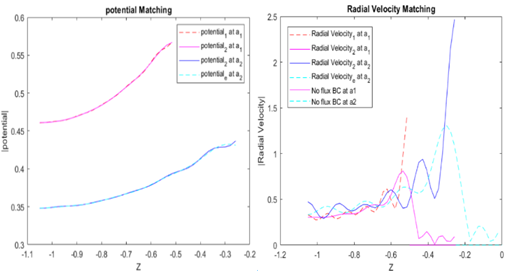
\includegraphics[width=0.75\linewidth]{figs/meem-matching.png}
    \caption{Matching for $N=M=K=11$ for benchmark geometry}
    \label{fig:meem-matching}
\end{figure}

Hydro coefficient convergence depends on the geometry: the benchmark shallow-water geometry of \cite{chau_inertia_2012} converges to within 0.25\% with only $N=M=K=4$, but RM3 requires $N=M=K>10$, shown in figure~\ref{fig:meem-convergence}. There, damping converges well at low frequencies but requires more harmonics at higher frequencies, while added mass has similar convergence across frequencies. 
\begin{figure}
    \centering
    \includegraphics[width=0.75\linewidth]{\matlabFilepath{31}}
    \caption{Convergence for $N=M=K=(3,5,10,20)$ for RM3}
    \label{fig:meem-convergence}
\end{figure}


\subsection{Numerical Notes}\label{sec:meem-numerics}
Note that radial eigenfunctions $R_{1n}^{i1}(r)$ and $R_{1m}^{i2}(r)$ contain the modified bessel function of the first kind $\mathrm{I}_0(b)$, which diverges for $b\rightarrow \infty$. This is the cause of the numeric overflow discussed in \ref{sec:meem}, where it was asserted that overflow occurs when the fluid region height to diameter ratio $\Delta z / D$ falls below some threshold. The threshold is a function of the number of harmonics $N_{harmonics}$ used in that region ($N$ for spar, $M$ for float), as well as the maximum argument to the \texttt{besseli} function in MATLAB before overflow, $b_{max}$:
\begin{equation}\label{eq:delta-z-min}
    \frac{\Delta z_{min}}{D} = \frac{\pi N_{harmonics}}{2b_{max}} \approx \frac{N_{harmonics}}{446}.
\end{equation}
By trial, $b_{max}$ is found to be $\approx 700.5$, close to the theoretical value of \texttt{log(realmax)} $\approx 709.8$ for exponential scaling. Since $N_{harmonics}=10$ gives adequate convergence for most geometries, this condition is trivially satisfied for nearly all floating bodies of practical relevance, but must still be added as a constraint to prevent the optimizer from exploiting the numerical divergence. In future work, if high-accuracy solutions are desired for large bodies close to the sea floor, exponentially scaled bessel functions could be used instead, with symbolic cancellation of the exponential scaler from the eigenfunction numerator and denominator.

Likewise, the vertical eigenfunction $Z_k^e$ for $k=0$ contains the $\cosh$ and $\sinh$ functions, which diverge for large values of $m_0h$ (high frequencies or deep water). Since the largest relevant value of $m_0h$ depends on the site rather than on the WEC design, it is not possible to add geometric constraints to prevent overflow as it was above. Therefore, the limit is derived analytically. %\hl{This formula hasn't been numerically checked yet}
\begin{equation}
    \lim_{m_0h\rightarrow\infty} Z_0^e(z)= \frac{\cosh^2(m_0h)}{\sqrt{2m_0h}}\exp\left(1+\frac{z}{h}\right)
\end{equation}
Plugging this into the first element of the bottom block of the b-vector results in 
\begin{equation}
    \lim_{m_0h\rightarrow\infty}b_{N+2M+1}=\frac{-a_2}{h-d_2} \sqrt{\frac{h}{2m_0}}\exp(-d_2m_0)
\end{equation}
\begin{figure}
    \centering
    \includegraphics[width=.75\linewidth]{\matlabFilepath{32}}
    \caption{Asymptotic b-vector for large $m_0h$}
    \label{fig:meem-b-limit}
\end{figure}

%\hl{Todo: add sentence describing this figure and what it tells us}

And the corresponding limit for the vertical coupling integral:
\begin{equation}
\begin{aligned}
    \lim_{m_0h\rightarrow\infty}\boldsymbol{\mathcal{Z}}_{m,k=0} &
    %= \int_{-h}^{-d_2} \vec{Z}_m^{i2 ~T}\vec{Z}_0^{e} dz 
    = h~\frac{\cosh^2(m_0h)}{\sqrt{2m_0h}}\cdot \frac{-1+(-1)^m\exp(1-\frac{d_2}{h})}{f_{m}} \\
    \text{where}~~f_m&= \begin{cases}
        1, & m=0 \\
        h^2\lambda_m^2+1, & m \geq 1
    \end{cases}
    \end{aligned}
\end{equation}
%\hl{check this formula}

A final numerical subtlety worth discussing is finite precision effects in calculating $m_k$. Bounds of $180^\textrm{o}\cdot[k-\frac{1}{2}, k]$ are placed on $m_kh$ in a root-finding algorithm to ensure the $k$th root is identified. Degrees are used instead of radians so asymptotes occur at rational values.

\subsection{Runtime and Computational Cost Scaling}

The runtime of the MEEM method is the time required to find the eigencoefficients, then obtain the hydrodynamic coefficients from eigencoefficients. First, a nonlinear root-finding algorithm runs $K-1$ times to generate the $m_k$ inputs used in the A-matrix and b-vector. Then $3N+8M+2K-11$ Bessel functions must be evaluated for the radial terms of the A-matrix. % if I change scaling of i1 from a2 to a1, it reduces by N-1. if I change scaling of i2 from a2 to (a1+a2)/2, it increases by 2*(M-1). So total would be 2N+10M+2K-12. see notebook p51.
The cost of evaluating vertical coupling integrals \ref{eq} is negligible since they are trigonometric. Linear solves scale almost cubically with matrix size, so this step scales with $(N+2M+K)^3$. The radial integrals for the c-vector do not require evaluating Bessel functions with any arguments that were not already evaluated for the A-matrix. For $N=M=K=10$, the simulation averages \hl{\#} ms on a Windows 10 laptop with a 2.5 GHz Intel i9 processor for a single frequency. Figure~\ref{fig:} shows the time breakdown. Most of the time is spent evaluating Bessel functions, so future code optimization should focus on speeding up Bessel evaluations, such as with lookup tables. \cite{chau_inertia_2012} proposes using the sparsity pattern to reduce matrix size from N+2M+K to 2M, but this seems low impact since the linear solve only takes a few percent of compute time. On the other hand, matrix size in a boundary element method solver is much larger (meshes may have 1000s of panels) and the linear solve drives computation cost. On the same machine, Capytaine boundary element method for the same geometry takes an average of 323 ms for a 710 panel mesh (1\% convergence). Thus, MEEM achieves a 10x time reduction over Capytaine.


\clearpage
\section{Dynamics and Control Module Details}

\subsection{Force Saturation}\label{sec:appendix-force-sat}
Section~\ref{sec:dynamics} introduced the use of describing functions to quantify the fundamental amplitude of non-sinusoidal force waveforms, which can achieve higher powers than the equivalent sinusoidal waveform for the same force limit.

The simulation permits the nonsinusoidal waveform to have a maximum fundamental a factor of $\frac{4}{\pi}$ above the force limit.
This coincides with the fundamental to peak ratio of a square wave, which is the limiting case both for the bang-singular-bang controller (a piecewise-discontinuous sine-square wave combination that \cite{hendrikx_optimal_2017} finds as the analytically optimal solution), and for the saturated sine controller (a piecewise-continuous sine-square wave combination that \cite{coe_initial_2020} finds as numerically optimal).
In fact, the optimization need not specify the exact nonlinear waveform, since under the describing function filtering hypothesis, only the fundamental matters for simulation purposes.
For hardware implementation purposes, the nonlinear controller can be obtained for the saturated-sine controller by the process outlined in \cite{mccabe_force-limited_2024}. 

MDOcean assumes that the saturated control impedance, and thus its fundamental, share the same phase as the optimal unsaturated controller (damping or reactive respectively).
This is optimal for the damping case, and slightly sub-optimal for the reactive case due to the presence of a small phase shift in the optimal saturated impedance and the matched impedance \cite{mccabe_force-limited_2024}.
The appropriate scale factor from the optimal unsaturated controller is found with numerical iteration. 

%Mathematically, a saturation factor $0< f_{sat}\leq 1$ is computed as the ratio between the fundamental amplitude of the saturated torque and the original unsaturated torque signal,
%\begin{equation}
%    f_{sat} = \min\left( \alpha\frac{\tau_{max}}{\tau}, 1\right),
%\end{equation}
%where $\tau_{max}$ is the maximum permissible generator torque and $\alpha$ is the ratio between the fundamental amplitude of the saturated waveform and the maximum torque $\tau_{max}$, using the describing function derived in \cite{mccabe_force-limited_2024},
%\begin{equation}
%    \alpha = \frac{2}{\pi} \left( \frac{F_p}{\tau_{max}}\sin^{-1}\frac{\tau_{max}}{F_p} +  \sqrt{1 - \left(\frac{\tau_{max}}{F_p}\right)^2} \right).
%\end{equation}
    
%When $\frac{F_p}{\tau_{max}}$ = 1 (no saturation), then $\alpha= 1$; when $\frac{F_p}{\tau_{max}} \rightarrow \infty$ (full saturation), then $\alpha= \frac{4}{\pi}$. This makes sense because $\frac{4}{\pi}$ is the harmonic amplitude of a unit square wave, and in full saturation the saturated signal approaches a square wave. $\alpha$ is plotted in Figure \ref{fig:alpha-fit}.

%The factor $f_{sat}$ describes the ratio of the saturated and unsaturated torque signal. Previous work \cite{mccabe_multidisciplinary_2022} implies that this is also the ratio of the saturated and unsaturated control gains, $m_{sat}$, but this is not the case because the WEC response also changes with saturation. 

% %Substituting $f_{sat}$ back into the equation of motion reveals that the control gain saturation multiplier $m_{sat}$ is the solution to a quadratic equation $a_q m_{sat}^2 + b_q m_{sat} + c_q = 0$. If the uncontrolled dynamics have a natural frequency $\omega_{n,u}$ and damping ratio $\zeta_u$, and the controlled unsaturated dynamics have natural frequency $\omega_n$ and damping ratio $\zeta$, then the quadratic coefficients can be expressed as:

% \begin{equation}\label{eq:abc-matrix}
%     \begin{bmatrix}
%         a_q \\ b_q \\ c_q
%     \end{bmatrix}
%     = 
%     \begingroup % keep the row spacing change local
%     \setlength\arraycolsep{2pt}
%     \begin{bmatrix} -4 & \frac{4}{f_{sat}^2} & \frac{1}{f_{sat}^2} & -1 & 0 & 0\\
%     8 & 0 & 0 & 2 & 8 & 2\\
%     -4 & -4 & -1 & -1 & -8 & -2 \end{bmatrix}
%     \endgroup
%     \begin{bmatrix} 
%  (\theta_1)^2  \\
%   (\theta_2)^2 \\
%    (\theta_3)^2 \\
%    (\theta_4)^2  \\
%    \theta_1 \theta_2 \\  
%     \theta_3 \theta_4
%     \end{bmatrix}
% \end{equation}
% where the basis vector $\vec{\theta}$ is a dimensionless function of the natural frequencies and damping ratios:
% \begin{equation}\label{eq:theta-basis}
%         \begin{bmatrix}
%   \theta_1  \\
%   \theta_2 \\
%    \theta_3 \\
%    \theta_4  \\
%     \end{bmatrix} =     \begin{bmatrix}
% ~ \overline{\omega} (\zeta_u - \overline{\omega}_n\zeta)  \\
%   \overline{\omega} ~\overline{\omega}_n \zeta \\
%   \overline{\omega}^2 - \overline{\omega}_n^2\\
%    \overline{\omega}_n^2 - 1  \\
%     \end{bmatrix}
% \end{equation}
% and the overlined frequencies indicate nondimensionalization by the uncontrolled natural frequency: $\overline{\omega} = \frac{\omega}{\omega_{n,u}}, \overline{\omega}_n = \frac{\omega_n}{\omega_{n,u}}$. The quadratic equation is then solved for $m_{sat}$, and of the two roots, the one that is real-valued and between 0 and 1 is used.

% The no saturation case ($f_{sat} = 1$) for \eqref{abc-matrix} yields $m_{sat}=1$. This confirms the expected behavior that when no force reduction is required, the powertrain coefficients can remain unchanged.

% Equations \eqref{eq:abc-matrix} and \eqref{eq:theta-basis} are an equivalent reformulation of \cite{mccabe_force-limited_2024}, which uses expressions for the complex reflection coefficient $\Gamma$ common in electrical engineering, rather than the damping ratio and natural frequency more common in mechanical engineering. The equivalence is:
% \begin{equation}
%     \Gamma = \frac{z-1}{z+1}, \quad z = \frac{2\theta_1 + i~ \theta_4}{-2(\theta_1+\theta_2) + i~(\theta_3+\theta_4)}
% \end{equation}
% % I am inputting zeta and omega_n corresponding to mechanical dynamcis when calculating m_sat, but I really should be inputting them corresponding to electrical dynamics. Maybe describe that?

% The gain saturation multiplier $m_{sat}$ is then used to modify the powertrain coefficients,
% \begin{align}
%     B_{p,sat} &= m_{sat} B_p, & K_{p,sat} &= m_{sat} K_p.
% \end{align}
% and these new control gains are then plugged into equation \eqref{eq:eom-freq-domain} to find the saturated displacement amplitude $X_{sat}$.

\clearpage
\subsection{Drag Model\label{sec:appendix-drag}}
Drag includes form drag (dominant impact), vortex shedding (moderate impact), and skin friction (minor impact) \cite{quartier_influence_2021}.
None of these three sources are captured in the MEEM hydrodynamics model due to the linear, irrotational, and inviscid assumptions respectively, so drag must be added separately.
As described in section \ref{sec:dynamics}, a describing function approximation is used.
This appendix describes an intricacy glossed over in section \ref{sec:dynamics} and entirely omitted in \cite{quartier_influence_2021}: the dependence of $\dot{x}_{wave}$ and thus $\dot{x}_{rel}$ across the width of the WEC in the direction of wave propagation $y$.
The authors of \cite{quartier_influence_2021} evaluate the wave velocity $\dot{x}_{wave}$ at the center of the WEC ($y=0$), which results in the drag damping coefficient $B_d$ becoming unrealistically low (even negative) at high frequencies and large wave heights.

A strip-theory approach avoids this issue by integrating the spatially-dependent infinitesimal drag force $dF_d$ over the wetted area $A_w$.
For a hollow cylinder of radius $R$ and inner radius $R_{in}$, this is expressed: 
% derived p156-159 notebook 3/10/25
% simplified p169-173 notebook 3/12/25
\begin{equation}\label{eq:drag-force-integral}
    F_d(t) = \int_{A_w} dF_d(y,t) = \int_{y=-R}^{R} w(y) P(y,t)dy
\end{equation}
where $w(y)$ is the local width of the WEC perpendicular to $y$:
\begin{equation}\label{eq:drag-width}
    w(y) = \begin{cases}
        2\sqrt{R^2-y^2}, & R_{in}<|y|<R \\
         2\sqrt{R^2-y^2}-2\sqrt{R_{in}^2-y^2}, &0<|y|< R_{in} \\
    \end{cases}
\end{equation}
and $P(y,t)$ is the local pressure acting vertically due to drag:
\begin{equation}\label{eq:drag-pressure}
    \begin{aligned}
    P(y,t) &= \frac{1}{2} \rho_w C_d ~\dot{x}_{rel}(y,t) ~|\dot{x}_{rel}(y,t)| \\
   &=  \frac{1}{2} \rho_w C_d ~\dot{X}_{rel}(y)^2 \sin(\omega t+\angle \dot{X}_{rel}(y)) ~\left| \sin(\omega t+\angle \dot{X}_{rel}(y))\right| \\
   &\approx  \frac{1}{2} \rho_w C_d ~\dot{X}_{rel}(y) ^2~\frac{8}{3\pi}\sin(\omega t+\angle \dot{X}_{rel}(y)) 
    \end{aligned}
\end{equation}
%notation: \dot{X}_rel here refers to the magnitude, not the complex phasor
% todo: I think technically the X's that I am taking the angle of should have a hat because they are complex

Moving into the frequency domain gives complex pressure $\hat{P}$:
\begin{equation}
\begin{aligned}
 \hat{P}(y,\omega)  &\approx \frac{1}{2} \rho_w C_d \frac{8}{3\pi}\alpha_v(y)^2 \dot{X}^2 e^{i\phi_\alpha(y)+i\angle\dot{X}}
    \end{aligned}
\end{equation}
where $\alpha_v(y)$ and $\phi_\alpha(y)$ are the amplitude and phase ratios, respectively, of the relative velocity and WEC velocity:
\begin{equation}\label{eq:drag-alpha-definitions}
\begin{aligned}
    \alpha_v(y) &\equiv \frac{\dot{X}_{rel}(y)}{\dot{X}} \\
    \phi_\alpha(y) &\equiv \angle
    \left(
        \frac{\hat{\dot{X}}_{rel}(y)}
            {\hat{\dot{X}}}
    \right)   
    = \angle\hat{\dot{X}}_{rel}(y) -  \angle\hat{\dot{X}} 
\end{aligned}
\end{equation}

Rewriting the relative velocity $\hat{\dot{X}}_{rel}(y)$ in equation \eqref{eq:drag-alpha-definitions} in terms of the finite depth incident wave velocity at a depth equal to the draft $\hat{\dot{X}}_{wave}(y) = \frac{H}{2} \frac{g k}{\omega} e^{-kT} e^{-iky}$ and the WEC velocity $\hat{\dot{X}}$ gives the following expressions for $\alpha_v^2(y)$ and $\phi_\alpha(y)$:

\begin{equation}
\begin{aligned}
    \alpha_v^2(y) &= 1 + r^2 e^{-2ky} - 2 r e^{-ky}  \sin\angle \hat{\dot{X}} \\
    \phi_\alpha(y) &= \mathrm{atan2}\left( \sin\angle \hat{\dot{X}} - r e^{-ky}, ~\cos\angle \hat{\dot{X}}\right) -  \angle\hat{\dot{X}}
\end{aligned}
\end{equation}
where $r = \dot{X}_{wave}(y=0)/ \dot{X}$ is the ratio of the wave velocity at the center of the WEC to the WEC velocity.
The drag force integral \eqref{eq:drag-force-integral} becomes:
\begin{equation}
    \hat{F}_d(\omega) \approx  \frac{1}{2} \rho_w C_d \frac{8}{3\pi}\dot{X}^2 e^{i\angle\hat{\dot{X}}}\int_{y=-R}^{R} w(y) \alpha_v(y)^2  e^{i\phi_\alpha(y)}dy
\end{equation}
noting that both the outer coefficient $e^{i\angle\hat{\dot{X}}}$ and the integral term $e^{i\phi_\alpha(y)}$ are complex phasors.
Setting $\hat{F}_{d}(\omega)%=\frac{1}{2}\rho_w C_d A_w \frac{8}{3\pi}  \dot{X}_{rel}(\omega)|\dot{X}_{rel}(\omega)|
=B_{d} \hat{\dot{X}} + K_{d} \hat{X}$ and solving for the coefficients yields
\begin{equation}\label{eq:drag-coeffs}
\begin{aligned}
B_{d} &= ~~~~~~\frac{4}{3\pi} \rho_w  C_{d} \dot{X} \int_{y=-R}^{R} w(y) \alpha_v(y)^2  \cos(\phi_\alpha(y))dy \\ % real part of c\_f
K_{d} &= - \omega~\frac{4}{3\pi} \rho_w  C_{d} \dot{X} \int_{y=-R}^{R} w(y) \alpha_v(y)^2  \sin(\phi_\alpha(y))dy \\ % -w times imag part of c\_f
\end{aligned}
\end{equation}

Plugging in the expressions for $w(y)$, $\alpha_v(y)$, and $\phi_\alpha(y)$ gives an integral with the following form:
\begin{equation}
\begin{aligned}
    &\int_{y=-R}^{R} w(y) \alpha_v(y)^2  e^{i\phi_\alpha(y)}dy \\
    = &\int_{y=-R}^{R} w(y) \sqrt{1 + r^2 e^{-2ky} - 2 r e^{-ky}  \sin\angle \hat{\dot{X}}} \left(f_3(\angle\hat{\dot{X}}) + f_2(\angle\hat{\dot{X}})re^{-ky}\right)  dy
\end{aligned}
\end{equation}
where $f_2$ and $f_3$ are trigonometric functions \hl{that I will derive during re-scrutineering, they are different for the cosine (Bd) vs sine (Kd).
For now before these integrals are derived, I assume the following:}
\begin{equation}
\begin{aligned}
    \phi_\alpha(y) &= 0 \\
    \alpha_v(y) &= \alpha_v(y=0) = 1 + r^2 - 2 r \sin\angle \hat{\dot{X}}
\end{aligned}
\end{equation}

Comparisons against WEC-Sim confirmed that this assumption yields more accurate results than the drag formulation used in \cite{quartier_influence_2021}, which uses an identical $\alpha_v(y)$ but assumes a different phase: $\phi_\alpha(y)=\phi_\alpha(y=0)$. 
At high frequencies and large wave heights, $r$ is large and $\phi_\alpha(y=0)$ exceeds $\pi$, causing the drag damping coefficient $B_d$ to be negative (non-dissipative), which is not realistic.
While setting $\phi_\alpha(y)=0$ does not guarantee that $B_d$ is always positive, it is found through testing to significantly reduce the risk of negative damping and to promote convergence of the drag loop.
In the optimization, any negative drag damping coefficents are set to zero.

% todo: write out full integral
%Like \cite{quartier_influence_2021}, this formulation evaluates the wave velocity $\dot{x}_{wave}$ at the center of the WEC rather than considering the variation in wave velocity along the direction of propagation as would be done with strip theory. This avoids cumbersome integral calculations at the cost of a small inaccuracy that will be quantified in section~\ref{sec:validation}.

With this approximation, the nonlinear time-domain drag equation is now a quasi-linear frequency-domain equation, since the state-dependence of the coefficients $B_{d}$ and $K_{d}$ prevents true linearity.
The solution for states $|\dot{X}|$ and $\angle \dot{X}$ can be obtained either through numerical iteration or analytical solution of the nonlinear equation\eqref{eq:eom}.
Iteration is chosen here, the same approach used for a frequency-domain drag simulation of floating offshore wind turbines \cite{hall_open-source_2022}.
Rather than employ a typical nonlinear root-finding algorithm, MDOcean simply uses the equation of motion \eqref{eq:eom} to obtain subsequent iterates.
This is a form of fixed point iteration where $x_k = g(x_{k-1})$ and is therefore guaranteed to converge as long as $|\frac{\partial g(x)}{\partial x}| < 1$ at the solution. %\hl{find a better place to cite for this besides wikipedia} \url{https://en.wikipedia.org/wiki/Root-finding_algorithm#Fixed_point_iteration_method}. 
Five to eight iterations on $|\dot{X}|$ and $\angle \dot{X}$ are typically required to converge all sea states to within 0.01~m, % from summer research slide 44 5/30/24
and a sample convergence plot is shown in Figure~\ref{fig:drag-convergence}.

In high-frequency sea states where there is substantial phase difference between $\dot{X}_{rel}$ and $\dot{X}$, $B_d$ occasionally becomes negative.
This does not violate the dissipative nature of drag \textit{overall}, because $F_d$ always opposes $\dot{X}_{rel}$ even if it does not oppose $\dot{X}$.
The non-dissipative effect of drag \textit{on the body} can be interpreted as modeling a second-order wave excitation force.
The effect would likely be mitigated if the position-dependence of the wave velocity were modeled, although this would require a difficult integration over the body surface and is left to future work.
Instead, if the negative drag exceeds the radiation damping and causes instability, the power for that sea state is zeroed.

Note that in the quasi-linear formulation, the lack of complete linearity means that the complex-conjugate reactive controller is technically no longer optimal.
The standard optimal control damping is derived by setting
\begin{equation}
0 = \frac{\partial P}{\partial B_p} = \frac{\partial \frac{1}{2} (B_p) \omega^2 |X|^2}{\partial B_p} = \frac{\partial \frac{1}{2} (B_p) \omega^2 |\frac{H\gamma/2}{(m+A_h)s^2+(B_h+B_d+B_p)s+(K_h+K_d+K_p)}|^2}{\partial B_p} 
\end{equation}
and the typical simplification $\frac{\partial B_d}{\partial B_p}=\frac{\partial K_d}{\partial B_p}=0$ must be replaced with the implicit dependence of $|X|$ on $B_d$ and $K_d$ from \eqref{eq:drag-coeffs}.
In practice, however, the standard complex conjugate controller was observed to produce nearly identical power as the one incorporating the more complicated dependence, so the standard is used for simplicity.

\begin{figure}
    \centering
    \includegraphics[width=0.75\linewidth]{\matlabFilepath{33}}
    \caption{Convergence plot for drag iteration}
    \label{fig:drag-convergence}
\end{figure}

\clearpage
\subsection{Slamming Amplitude}\label{sec:appendix-slam}
In regular waves of height $H$, the conditions for slamming can be derived by comparing the vertical position of the bottom of the WEC, $x(t)-\Delta z_{slam,bot}$, with the wave elevation $\zeta(y,t)$, which depends on the horizontal position coordinate $y$.
To prevent slamming, the criteria
\begin{equation}\label{eq:slamming-time-domain}
\begin{aligned}
    x(t) - \Delta z_{slam,bot} &< \zeta(y,t) \\ 
    |X|\cos(\omega t+\angle X) - \Delta z_{slam,bot} &< \frac{H}{2}\cos(\omega t - k y)
\end{aligned}
\end{equation}
must be true at all times and over all positions where the body could exit the waves, $-D/2<y<D/2$.
Note that this expression assumes a sinusoidal waveshape but still applies for irregular waves if a wave-by-wave approach \cite{lin_fast_2025} is utilized.
Manipulation yields the criterion $|X|<X_{slam}$, where the critical amplitude before slamming occurs $X_{slam}$ is
\begin{equation}
\begin{aligned}
    X_{slam} &= \sqrt{\Delta z_{slam,bot}^2-\left(\frac{H}{2}\sin\theta\right)^2 } - \frac{H}{2} \cos\theta \\
    \textrm{where } \theta &= \max\left(0,~ \frac{-kD}{2}+|\pi-\angle X|\right).
\end{aligned}
\end{equation}
This expression reduces to the simple limits $\Delta z_{slam,bot}-H/2$ and $\Delta z_{slam,bot}+H/2$ for short wavelengths $(\theta=0)$ and long wavelengths $(\theta=\pi)$ respectively.
These limits are also the minimum and maximum nonzero critical slamming amplitudes for any design and wave condition.
For intermediate wavelengths, the variable $\theta$ accurately accounts for the effect of body diameter and the phase offset of body motion from the waves.
Intuitively, $\theta$ represents how high up the free surface the bottom of the WEC is allowed to get before the edge exits the water, with $\theta=\pi$ allowing the body to get all the way to the wave crest (top) and $\theta=0$ requiring the float to remain fully below the trough (bottom).
Figure~\ref{fig:slam} visualizes the relationship using the nondimensional parameter $X^*$ to map the slamming amplitude onto the range $[-1,1]$.
This reveals that besides increasing the draft, increasing $\theta$ can prevent slamming, for example by decreasing the diameter or adjusting $\angle X$ via control.
If $\Delta z_{slam,bot}<H/2\sin\theta$, slamming occurs even for a stationary body, and the critical slamming amplitude is set to zero to indicate an unviable design.
\begin{figure}
    \centering
    \includegraphics[width=1\linewidth]{\matlabFilepath{34}}
    \caption{Nondimensional critical slamming amplitude}
    \label{fig:slam}
\end{figure}
%\hl{add description of similarities and differences of this to Budal's upper bound}

Separately, there exists a symmetrical counterpart to the above slamming condition, where in addition to requiring the bottom the WEC to remain below the waves, one can require that the top of the WEC remains above the waves, preventing full submersion. 
Analogous to \eqref{eq:slamming-time-domain}, we obtain:
\begin{equation}\label{eq:top-slamming}
    x(t) + \Delta z_{slam,top} > \zeta(y,t)
\end{equation}

Conceptually, both the bottom-slamming requirement \eqref{eq:slamming-time-domain} and the top-slamming requirement \eqref{eq:top-slamming} must be applied to both the float and the spar for a total of 4 constraints for each sea state.
However, the top-slamming and bottom-slamming requirement for each body is aggregated into a single constraint for each sea state, using $\Delta z_{slam}=\min(\Delta z_{slam,top}, \Delta z_{slam,bot})$, where the values for $\Delta z_{slam,top}$ and $\Delta z_{slam,bot}$ were given in \sectionautorefname~\ref{sec:dynamics}.
\hl{(Note: There also might be a slight difference in the way theta would be calculated for top and bottom slamming, this will be checked during re-scrutineering).}
%However, implementing the top-slamming requirement for the float becomes redundant of the float bottom-slamming requirement due to the parameter choice $T_{f,2}/h_f=1/2$ enforcing equal draft and above-water height.
%If $h_f$ were added as an independent design variable, the float top-slamming requirement would become necessary to implement, although note that the normalized value of $\frac{dLCOE^*}{dT_{f,2}/h_f}$ in \figureautorefname~\ref{fig:param-sens-J-star-tornado} is less than -0.1, suggesting that the addition of $h_f$ as a design variable would provide little benefit and is therefore low priority.
Meanwhile, it is only required to implement the slamming constraint for the float not the spar because \reqref{base_dynamic} and \reqref{tops_dynamic} already ensure, respectively, that the bottom of the spar remains below the bottom of the float and that the top of the spar remains above the top of the float across all dynamic conditions.
Since the float slamming requirement applies for all $-D_f/2<y<D_f/2$ and the spar diameter is always smaller than the float's (via \reqref{float_spar_diam}), the spar slamming requirements are redundant. This reduces the number of slamming constraints per sea state from four to one.

Following section~\ref{sec:discussion}, it is interesting to analyze the impact of the more complicated intermediate-wavelength slamming model compared to the simple and conservative short-wavelength model ($X_{slam}=\Delta z_{slam}-H/2; X^*=-1$).
Relevant model values for the minimum-LCOE float design are plotted for each sea state in \figureautorefname~\ref{fig:slamming-validation}.
Although the intermediate wavelengths ($X^*>-1$) occur for many operational sea states, those sea states are not the ones where the slamming constraint is active (where $X_{slam}/X-1 \approx 0$) because in this JPD, large amplitude waves occur only at high periods.
If the more conservative short-wavelength model is used, the slamming constraint appears violated with a value of $-0.08$ (the small blue portion at the top of the rightmost subplot at $T_e=12.5$ s, $H_s=6.75$ m), indicating that the float draft would need to increase by around 8\% to prevent slamming.
This would increase total material cost by around 2\% and LCOE by around 0.5\%, an effect likely dwarfed by other sources of uncertainty.
Thus, in this case the more complicated, less conservative slamming model has only a minor impact on the optimization, although more substantial impact is expected in seas with co-occurring large-amplitude and low-to-moderate-period waves. 
\begin{figure}
    \centering
    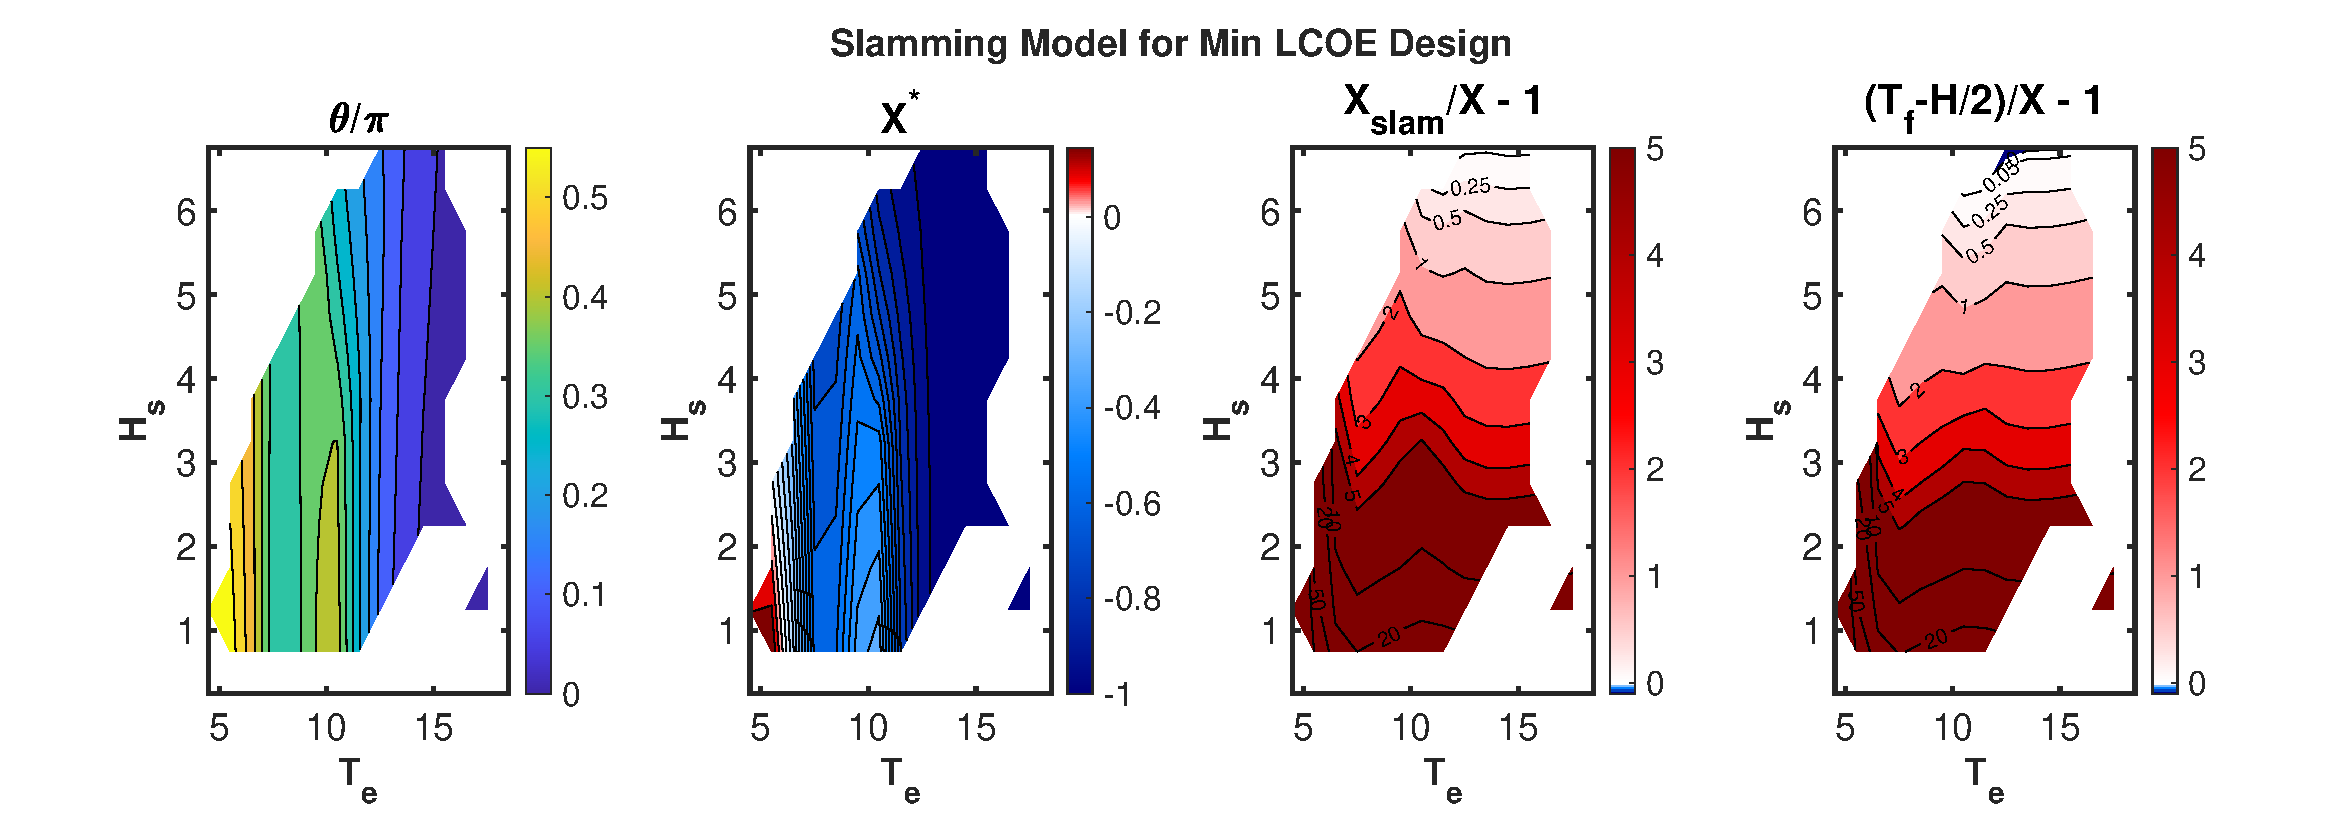
\includegraphics[width=1.1\linewidth]{figs/slam_validation.pdf}
    \caption{Slamming Model Comparison for Minimum LCOE Design in Operational Sea States}
    \label{fig:slamming-validation}
\end{figure}

\subsection{Dynamic Validation}\label{sec:appendix-dynamic-validation}
A WEC-Sim parallel multiple condition run is performed in accelerator mode for 3100s with a 100s ramp time using the ode4 solver and a 10 ms timestep, with the default mass properties of the WEC-Sim RM3 tutorial.
Each of the 210 sea states are simulated individually. %Table~\ref{tab:dynamic-validation} and 
Figure~\ref{fig:dynamic-validation} compares the results.
% \begin{table}
%     \centering
%     \begin{tabular}{|c|c|c|} \hline 
%          Power Percent Error: Average, Maximum&  $C_d=0$& $C_d=1$\\ \hline 
%          WAMIT&  1.90\%, 1.96\%& 5.21\%, -70\%\\ \hline 
%          MEEM&  -6.30\%, -14\%& -2.79\%, -80\%\\ \hline
%     \end{tabular}
%     \caption{Dynamic validation showing error in a variety of modeling assumptions}
%     \label{tab:dynamic-validation}
% \end{table}
\begin{landscape}
\begingroup
\begin{figure}
\centering
\begin{tabular}{c m{1em} | >{\centering\arraybackslash}m{.5\linewidth} >{\centering\arraybackslash}m{.5\linewidth} }
  && \multicolumn{2}{c}{Drag Coefficent}\\
         && $C_d=0$& $C_d=1$\\ \hline
    \multirow{2}{*}[-3em]{\rot{Hydro Coeffs}} &\rot{Identical}& \includegraphics[width=\linewidth]{\matlabFilepath{36_a}} & \includegraphics[width=\linewidth]{\matlabFilepath{36_b}} \\
     &\rot{Different} & \includegraphics[width=.5\linewidth]{example-image-a} & \includegraphics[width=\linewidth]{\matlabFilepath{36_d}} \\
\end{tabular}
\caption{Dynamic validation showing error in a variety of modeling assumptions}
\label{fig:dynamic-validation}
\fillandplacepagenumber
\end{figure}
\endgroup
\end{landscape}


\clearpage
\section{Structures Module Details}
\label{sec:appendix-structures}
Inputs to the structures module include forces, bulk and structural dimensions, and material constants.
It outputs a factor of safety for each limit case.
First, it obtains equivalent section properties based on the plate and stiffener dimensions.
Second, it relates applied loads to stresses and deflection using analytical solutions to structural boundary value problems obtained from the well-known Roark's handbook \cite{young_roarks_2001} and the references therein.
Finally, it utilizes design standards from organizations like Det Norske Veritas, the American Bureau of Shipping, and the American Iron and Steel Institute to develop limit state expressions for each possible failure mode of each major structural element under each design load case. %\hl{cite DNV standards, RM3 report+new structures addendum, some WEC structures paper, say that typically structures are designed to an ultimate limit and made of stiffened steel because it is efficient way to handle the spread out surface load of the ocean. Also note that for consistency with the RM3 report, welded joints are assumed everywhere, although using pinned joints such as a rod end attachment on the float and reaction plate tubular support structures could enhance structural efficiency.}

\subsection{Equivalent Section Properties for Stiffened Plates}\label{sec:equivalent-thickness}
Stiffeners are structural elements, frequently with I or T profiles, that can be welded or riveted to flat plates to provide additional load-carrying capacity and prevent buckling.
Stiffened plates are common in marine and aerospace structural design because they are an efficient way to carry spatially distributed fluid loads.
To analyze these compound sections, equivalent properties can be established that describe the overall bending stiffness of the combined section as if it were a simple uniform section, while still utilizing the maximum distance from the neutral axis of the irregular section to accurately determine stress.
Figure~\ref{fig:stiffened-plate} illustrates the concept of equivalent thickness for a stiffened plate.
\begin{figure}
    \centering
    \includegraphics[width=\linewidth]{figs/stiffener_equivalence.pdf}
    \caption{Equivalent thickness for a stiffened plate}
    \label{fig:stiffened-plate}
\end{figure}

Specifically, the equivalent thickness of the plate $t_{eq}$ is derived by equating the stiffened section's second moment of area per unit width with that of a uniform section:
\begin{equation}
    \int z^2dz = \frac{t_{eq}^3}{12}
\end{equation}
Next, deflection of the stiffened plate is equal to the deflection of the equivalent unstiffened plate with flexural rigidity $D_{eq}$:
\begin{equation}
    D_{eq} = \frac{E~  t_{eq}^3}{12(1-\nu^2)}
\end{equation}

The maximum stress $\sigma$ of the stiffened plate is then:
\begin{equation}\label{eq:plate-stress}
    \sigma= 12M z_{max}/t_{eq}^3
\end{equation}
where $M$ is the maximum moment per unit length and $z_{max}$ is the maximum distance from the neutral axis of the stiffened section.
This parallels the stress for an unstiffened plate of thickness $t$, which is $\sigma=6M/t^2 = 12 M(t/2)/t^3$.

Note that this equivalent-thickness method of accounting for stiffeners assumes that as a whole, the stiffener-plate system deflects like a single plate element, rather than as set of multiple plate elements separated by stiffeners.
This is a reasonable assumption when the stiffeners are small and densely spaced with respect to the plate, but breaks down if the stiffeners come to dominate the system.
The so-called effective breadth ratio $\rho$ is used to quantify the validity of this assumption, where the equivalent-thickness method requires $\rho=1$:
\begin{equation}
   \rho = \rho_\lambda \rho_\psi
\quad 
\rho_\lambda = \begin{cases}
        1, & \lambda\leq 0.673 \\
        \frac{1-0.22/\lambda}{\lambda}, & \lambda > 0.673
    \end{cases} \quad
    \rho_\psi = \begin{cases}
        1, & \psi> -0.236 \\
        \frac{1}{2}+\frac{1}{3-\psi}, & \psi \leq -0.236
    \end{cases} 
\end{equation}
The effective breadth ratio depends on the slenderness factor $\lambda$ and load distribution factor $\psi$, found as follows:
\begin{equation}
\begin{aligned}
    \lambda &= \frac{1.052}{\sqrt{k_{buckle}}} \frac{w}{t} \sqrt{\frac{f_1}{E}} \\
    \psi&=\frac{f_2}{f_1}
    \end{aligned}
\end{equation}
with $t$ referring to the plate unstiffened thickness, $w$ as the distance between stiffeners, $f_1$ as the maximum compression stress along the width, and $f_2$ as the maximum tension stress along the width (or minimum compression stress, if there is no tension).
By convention, compression stress is positive and tension is negative, so $\psi$ ranges from $-\infty$ to $+1$.
The plate buckling coefficient $k_{buckle}$ is expressed as:
\begin{equation}\label{eq:k-buckle}
  k_{buckle} = 4+2\left(1-\psi\right)^3+2\left(1-\psi\right)
\end{equation}
This effective breadth procedure follows the American Iron and Steel Institute design manual \cite{american_iron_and_steel_institute_cold-formed_1991}.
Rather than enforcing $\lambda<0.673$, corresponding with $\rho_\lambda=1$, MDOcean more flexibly requires $\lambda<0.809$, corresponding to $\rho_\lambda=0.9$ and thereby capping the error due to insufficient slenderness at around 10\%.
MDOcean also uses $k_{buckle}=4$, the minimum value that equation \eqref{eq:k-buckle} can take on, conservatively maximizing the slenderness factor $\lambda$.

Broadening the design space to allow for more dominant stiffeners with higher slenderness factors would require modeling the stiffener-plate system not as a plate with the stiffeners absorbed into an equivalent thickness, but as individual stiffeners with the plate absorbed into the effective breadth.
That model has other complexities such as the shear lag phenomenon so is left to future extensions \cite{wierzbicki_lecture_2013,american_iron_and_steel_institute_cold-formed_1991}.

%\hl{Describe how this informs the lower design variable bounds on the structural stiffnesses.}

\subsection{Float}
The float is composed of 12 watertight stiffened shells in the shape of trapezoidal prisms.
Each shell consists of a top and a bottom trapezoidal plate, and an inner, an outer, and two side rectangular plates.
All edges are welded.
Rather than model the deflections of each edge and apply compatibility, for simplicity the edges of each plate are conservatively modeled as fixed.
The top and bottom plates are the only ones with external heave loads, arising from the float-spar tubular connection and the hydrodynamic pressure respectively.

The trapezoidal plates are isosceles trapezoids with smaller base $b_1 = \pi D_{f,in}/12$, larger base $b_2=\pi D_f/12$, and perpendicular height $h_0=(D_f-D_{f,in})/2$ (see \figurename~\ref{fig:trapezoid}).
The references consulted do not contain structural results for trapezoidal plates, so geometric intuition is used to scale available solutions.
For example, \cite{young_roarks_2001} contains models for rectangular plates under perpendicular loading.
They show that the maximum bending stress $\sigma$ scales with the square of the shorter side length, $x_{min}^2$. % in rectangular plates, with the square of the altitude in triangular plates, and with the square of the radius in circular sectors. 
This makes sense because for fixed-edge plates with distributed loads, it is the square of the minimum distance from an edge to the point of highest deflection, $(x_{min}/2)^2$, that geometrically sets the maximum curvature, so $\sigma\sim x_{min}^2$.
For trapezoids, one then expects approximate rectangles ($b_2/b_1\approx1$) to have $x_{min}=\min(b_1,h_0)$, short trapezoids ($h_0<b_1)$ to have $x_{min}=h_0$, tall trapezoids ($h_0\gg b_2$) to have $x_{min}=b_1$, and intermediate trapezoids to have an $x_{min}$ that depends on the trapezoid slope.
The nominal RM3 design falls into this intermediate case, with $b_1\approx1.7$~m, $b_2\approx5.2$~m, and $h_0\approx6.8$~m.
These dimensions are shown in figure~\ref{fig:trapezoid}.

\begin{figure}
    \centering
    \includegraphics[width=0.75\linewidth]{\matlabFilepath{37}}
    \caption{Trapezoidal float plate with inscribed circle used to determine $x_{min}$}
    \label{fig:trapezoid}
\end{figure}

To approximately capture the dimensions of a trapezoid which effectively set the deflection curvature and therefore stress, $x_{min}$ is set to the diameter of the largest circle that can be inscribed in the trapezoid tangent to the shorter base $b_1$.
This inscribed circle scheme satisfies all limit cases mentioned above and can be calculated as
\begin{equation}
    x_{min} = \begin{cases}b_1 \left( m + \sqrt{1+m^2}\right), & h_0 \geq \sqrt{b_1b_2} \\ h_0, & h_0 < \sqrt{b_1b_2}\end{cases}
\end{equation}
where $m=(b_2-b_1)/(2h_0)$ is the slope of the trapezoid.
The expression is continuous at $h_0=\sqrt{b_1b_2}$, the point where the inscribed circle becomes tangent to base $b_2$ in addition to $b_1$.
Continuity of the model across the design space avoids problems in the gradient-based optimization due to undefined gradients.
The inscribed circle model gives $x_{min}\approx2.2$~m for the nominal float design.
In addition to the shorter side length $x_{min}$, stress in a fixed-edge rectangular plate also depends weakly on the longer side length of the plate $x_{max}$, which for the trapezoid is taken as
\begin{equation}
    x_{max} = \begin{cases} h_0,& h_0 \geq \sqrt{b_1b_2} \\ \frac{b_1+b_2}{2} + h(1-\sqrt{1+m^2}), & h_0 < \sqrt{b_1 b_2}\end{cases}
\end{equation}
using a similar inscribed circle scheme to maintain continuity.
Under a distributed pressure $q$, the bottom plate maximum moment per unit length is then $M_{bot}=\beta q x_{min}^2$ for $\beta$ tabulated as a function of $x_{max}/x_{min}$ in reference \cite{timoshenko_theory_1959}, and the bending stress is found by plugging this moment into equation~\eqref{eq:plate-stress}.

The top float plate has equivalent thickness $t_{f,top,eq}$ and the same dimensions and edge fixity as the bottom plate.
Unlike the uniform pressure on the bottom plate, the top plate is subject to the welded tubular float-spar attachment force and moment, modeled as a load distributed over a small circle of radius $r_0$, where $r_0$ is assumed to be at least half the thickness.
Under these conditions, either the stress at the center $\sigma_{cent}$ or along the longer edge $\sigma_{edge}$ may dominate:
\begin{equation}
    \begin{aligned}
    \sigma_{edge}&= \frac{3W}{2\pi t_{f,top,eq}^2}\left( (1+\nu)\ln\frac{2x_{min}}{\pi r_0}+\beta_1\right)\\
        \sigma_{cent}&=-\beta_2 W/t_{f,top,eq}^2
    \end{aligned}
\end{equation}
using $\beta_1$ and $\beta_2$ tabulated as a function of $x_{max}/x_{min}$ in \cite{young_roarks_2001}.
The bending moment per unit length is then found as $M_{top}=\sigma_{edge}t_{f,top,eq}^2/6$. \hl{(Note: this equation gives unusual results so it is not currently used. The top plate thickness is set via scaling of the bottom plate thicknesses. Will be debugged during scrutineering.)}

The other float plates besides the top and bottom ones experience only the edge reaction moments from the top and bottom plates, with no additional external loads in heave. 
Assuming that the maximum allowable stress is the same in all float plates, the required side plate thickness can be found by simply scaling the input float bottom plate thickness using the float thickness ratios in the nominal RM3 design. This prevents the need for a separate structural analysis of the side plates.

\subsection{Damping Plate}
For an annular plate with free outer radius $a$ and fixed inner radius $b$, the nondimensional plate deflection $\overline{\delta}_{plate}$ and bending moment $\overline{M}_r$ can be calculated as a function of plate aspect ratio $b/a$ for various load cases.
In this case, the plate is loaded by a distributed load (subscript $dis$) equal to $F_{heave}$, and a concentrated load (subscript $con$) at four equidistant points along the edge, equal to the tubular support reaction force $F_{tube}$.
Formulas for the concentrated loading are given in \cite{boedo_corrected_1998}, and formulas for distributed loading are given as case 2L of table 11.2 in \cite{young_roarks_2001}.
The 24 radial plate stiffeners are taken into account with the procedure described in section~\ref{sec:equivalent-thickness}, producing equivalent flexural rigidity $D_{eq}$ and equivalent section modulus $S_{eq}$.
The tube force $F_{tube}$ is statically indeterminate and is solved with compatibility by equating the plate and tubular support displacements, $\delta_{plate}=\delta_{tube}$, where the tube displacement is expressed in terms of its bending stiffness $K_{tube}$.
This results in the following expression for the radial plate bending stress $\sigma_r$:
\begin{equation}
    \sigma_r =  \frac{F_{heave}}{S_{eq}} \left( 
    \overline{M}_{r,dis} + \overline{M}_{r,con} \frac{\overline{\delta}_{plate,dis}}{\frac{D_{eq}}{a^2K_{tube}} - \overline{\delta}_{plate,con}}
    \right)
\end{equation}

The critical buckling stress $\sigma_{buckle}$ is found according to \cite{american_bureau_of_shipping_requirements_2022}.
The ultimate stress is then $\sqrt{\sigma_Y \sigma_{buckle}}$  \cite{wierzbicki_lecture_2013-1} and the endurance limit is taken as half of ultimate.
The factor of safety is then the ratio of the maximum (ultimate or endurance, depending on the design load case) stress to the radial plate bending stress.
The procedure is summarized in Figure~\ref{fig:damping-plate-flowchart}.
\begin{figure}
    \centering
    \includegraphics[width=1\linewidth]{figs/damping_plate_flowchart.pdf}
    \caption{Calculation process flowchart for the damping plate structural assessment}
    \label{fig:damping-plate-flowchart}
\end{figure}
%\hl{Todo: typeset equations for all the inputs with leftmost boxes: Seq, Deq, Ktube, the nondim variables, and sigma buckle.

%Todo: describe the plots of plate stress/deflection over space, maybe add dots in the 4 corners showing the point of load application}
\begin{figure}
    \centering
    \includegraphics[width=0.5\linewidth]{\matlabFilepath{39}}
    \caption{Damping plate moment}
    \label{fig:damping-plate-moment}
\end{figure}
\begin{figure}
    \centering
    \includegraphics[width=0.5\linewidth]{\matlabFilepath{40}}
    \caption{Damping plate deflection}
    \label{fig:damping-plate-deflection}
\end{figure}
In Figure~\ref{fig:damping-plate-maxs}, peak stress and deflection are plotted as a function of damping plate aspect ratio, normalized by their values in the nominal design.

\subsection{Column}
As stated in \ref{sec:structures}, the column's small slenderness ratio means that both axial compression and global Euler buckling must be taken into account.
Meanwhile, the hydrostatic pressure at the bottom creates a substantial compressive hoop stress.

The Euler critical buckling force $F_{crit}$ is:
\begin{equation}
    F_{crit} = \frac{\pi^2 E I}{(K_{end} L)^2}
\end{equation}
where $E$ is the Young's modulus, $I$ is the second moment of area, $K_{end}=2$ is the end condition (fixed-free since the hydrostatic rotational stiffness provides a restoring moment at the surface), and $L$ is the beam length, set to $h_s$ the full spar height.
The spar factor of safety $FOS$ to prevent yield and global buckling under the combined loading is \cite{american_bureau_of_shipping_requirements_2022}:
\begin{equation}
    FOS = \frac{\sigma_{s,max}}{\sigma_s} = \frac{\sigma_Y \frac{\zeta + \sqrt{\zeta^2+4\omega}}{2}}{\frac{F}{A} + q}
\end{equation}
where $\zeta$ and $\omega$ are defined as follows:
\begin{equation}
\begin{aligned}
     \zeta &= 1 - P_r(1 - P_r)~\sigma_Y~\frac{F_{crit}}{A} - \frac{\sigma_\theta}{\sigma_Y} \\
    \omega &= \frac{\sigma_\theta}{2\sigma_Y}  (1 - \frac{\sigma_\theta}{2\sigma_Y})
\end{aligned}
\end{equation}
and the hoop stress $\sigma_\theta$ is 
\begin{equation}
     \sigma_\theta = \frac{qD_s}{2~t_{s,r}}
\end{equation}
$P_r$ is a constant and $q$ is the distributed hydrosatic pressure at the bottom of the spar.
These equations assume that the spar is compact, meaning that local buckling of the tube as a plate element is not a concern \cite{american_bureau_of_shipping_requirements_2022}.
%These stresses are combined into the von Mises stress $\sigma_{vm}$ as defined in equation \eqref{von}. 
% \begin{equation}
% \begin{split}
%     \sigma_{vm}^2 = \frac{1}{2} \left( (\sigma_{11} - \sigma_{22})^2 + (\sigma_{22} - \sigma_{33})^2 + (\sigma_{33} - \sigma_{11})^2 \right) \\ + 3 (\sigma_{12}^2 + \sigma_{23}^2 + \sigma_{31}^2)
%     \label{von}
% \end{split}
% \end{equation}

% Three yield factors of safety $FOS_y$ (for the float, vertical column, and damping plate) and one buckling factor of safety $FOS_b$ (for the vertical column) are computed for each of two forces (the powertrain force $F_p$ and the hydrodynamic excitation force $F_h$). This gives a total of eight FOS:
% \begin{equation}
% \begin{aligned}
%     FOS_{y~{i,j}} = \frac{\sigma_y}{\sigma_{vm,ij}} ~~&~~
%     FOS_{b,j} = \frac{F_{crit}}{F_j} \\
%     i = 1..3, ~& j = 1..2
% \end{aligned}
% \end{equation}
\clearpage
\section{Economic Model Details}
\label{sec:appendix-econ}
The capital cost is a simple summation of the device costs, which depend on the WEC design, and the balance of system and financial costs $C_0$, which are assumed constant.
\begin{equation}
	CAPEX = N_{WEC}C_{unit} + C_0
\end{equation}
The value for $C_0$ is obtained as the development, infrastructure, profit margin, installation, and contingency costs in the RM3 cost breakdown structure \cite{neary_reference_2014}.

Unit device costs include that of the drivetrain $C_{drv}$, generator $C_{gen}$, structural material $C_{struct}$, and a fixed cost $C_{fixed}$ for components like mooring whose scaling with design is not captured here:
\begin{equation}
    C_{unit} =  C_{drv}(P_{pk,elec}) + C_{gen}(\tau) + C_{struct}(V_{struct}) + C_{fixed}
\end{equation}
The drivetrain cost model used in \cite{RM3} comes from an unpublished design and cost estimate for a hydrualic PTO that ReVision Consulting performed in 2011.
The ReVision study estimated unit costs for a 100~kW peak device at quantity 1 and 100.
The reference model project scaled the costs linearly with peak power (except for the riser cable and control system, whose cost does not scale with power) and found component-level progress ratios to describe the economies of scale.
%\hl{describe my force power scaling}
% is taken from the NREL System Advisory Model for the RM3 hydraulic system, and scales slightly less than linearly with peak power rating \cite{nakhai_techno-economic_2022}:
% \begin{equation}
%     C_{drv} = 7.216 P_{pk,elec}^{0.91}
% \end{equation}
% Generator cost estimates come from linear curve fits of commercial electric machines performed in \cite{nakhai_techno-economic_2022}. Induction and permanent magnet machines have different costs, each scaling linearly with the peak torque rating, so the cheaper of the two is chosen with a torque threshold:
% \begin{equation}
%     C_{gen} = \begin{cases}
%     80.86 \tau + 1032, & 0~\leq\tau <47~\text{Nm, ~~~~induction generator} \\
%     9.151 \tau + 4386, & 47\leq\tau \leq 4000~\text{Nm, permanent magnet generator}
%     \end{cases}
% \end{equation}
%While the RM3 report only specifies a 286 kW power rating and does not specify the maximum PTO torque, the maximum PTO torque is calculated as
The structural cost is the product of the structural volume and the material price $p_M$:
\begin{equation}
    C_{struct} = p_M V_{struct}
\end{equation}

%The operational expenditure $OPEX$ scales via power law with the number of WECs. The exponent and operational price coefficient $p_{op}$ are determined via a least-squares curve fit to (\hl{cite RM3 CBS data}):
%\begin{equation}
  %  OPEX = p_{op} N_{WEC}^{0.4433}
%\end{equation}
The annual energy production in kilowatt-hours is the average electrical power from equation~\eqref{eq:power-elec} multiplied by the number of hours per year.

To better see the dependence of LCOE on design, one can divide out the constant factors and introduce various price constants $p_{(*)}$.
Assuming a fixed $N_{WEC}, FCR,$ and $\eta_{op}$, the LCOE model then scales as:
\begin{equation}\label{eq:LCOE-scale}
  LCOE = \frac{p_\tau \tau + p_{P}P_{pk,elec}^{0.91} + p_{struct} V_{struct} + p_0}{P_{avg,elec}}
\end{equation}
The values of price and cost constants are given in \sectionautorefname~\ref{sec:appendix-parameters}.


% To see the effect of changes from some nominal design \hl{(finish this sentence, and maybe change nominal ratios to bar variables for easier readability)}
% \begin{equation}\label{eq:LCOE-scale}
%     \frac{LCOE}{LCOE_{nom}} = \frac{p_\tau \frac{\tau}{\tau_{nom}} + p_{P}\frac{P_{pk,elec}^{0.91}}{P_{pk,elec,nom}^{0.91}} + p_{struct} \frac{V_{struct}}{V_{struct,nom}} + 1}{\frac{P_{avg,elec}}{P_{avg,elec,nom}}}
% \end{equation}

\clearpage
\section{Parameters}
\label{sec:appendix-parameters}
\begin{table}[ht]
\centering

%\setlength{\tabrowsep}{} % default value:
\renewcommand{\arraystretch}{1.4}

\begin{tabular}{c>{\centering\arraybackslash}p{0.35\linewidth}>{\centering\arraybackslash}p{0.3\linewidth}c}
\textbf{Parameter} & \textbf{Description} & \textbf{Value} & \textbf{Units}  \\ \hline
$\rho_w$ & Seawater density& 1000 & kg/$m^3$  \\ 
$g$& Acceleration of gravity& 9.8 & m/$s^2$  \\ 
$h$& Water depth & 100 & m  \\ 
JPD& Wave joint probability distribution & read from file \cite{janzou_sam_2022}  &\%  \\ 
$H_s$ & Wave height \cite{janzou_sam_2022}& 0.25 : 0.5 : 6.75  & m  \\ 
$H_{s,struct}$ & 100 year wave height \cite{berg_extreme_2011}& [13.4, 18.8, 24.2, 30.1, 24.2, 18.8, 13.4] & m  \\ 
$T$& Wave energy period \cite{janzou_sam_2022}& 4.5 : 1 : 18.5  & s  \\ 
$T_{struct}$ & 100 year wave peak period \cite{berg_extreme_2011}& [5.57 8.76 12.18 17.26 21.09 24.92 31.70] & s  \\ 
$\sigma_y$ & Material yield strength& 248 & MPa  \\ 
$\rho_m$ & Material density& 7850 & kg/$m^3$  \\ 
$E$& Material Young's modulus& 200 & GPa  \\ 
$cost_m$ & Material cost& 1.89 & \$/kg \\ 
%$t_{ft}$ & \begin{tabular}[c]{@{}c@{}}Surface Float Top Plate\vspace{-1.5 mm} \\ Thickness\end{tabular} & 0.013 & m  \\ 
%$t_{fr}$ & \begin{tabular}[c]{@{}c@{}}Float Radial Wall\vspace{-1.5 mm} \\ Thickness\end{tabular} & 0.011 & m  \\ 
%$t_{fc}$ & \begin{tabular}[c]{@{}c@{}} Float Circumferential\vspace{-1.5 mm} \\ Gusset Thickness\end{tabular} & 0.011 & m  \\ 
%$t_{fb}$ & Float Bottom Thickness & 0.014 & m  \\ 
%$t_{sr}$ & Vertical Column Thickness & 0.025 & m  \\ 
%$B_{min}$ & Minimum Buoyancy Ratio & 1 & -  \\ 
$FOS_{min}$ & Minimum factor of safety& 1.5 & -  \\ 
$D_{d_{min}}$ & Minimum damping plate diameter & 30 & m  \\ 
$FCR$ & Fixed charge rate& 10.8 & \%  \\ 
$N_{WEC}$ & Number of WECs in array& 100 & -  \\ 
$D_{d}/{D_{s}}$ & Normalized damping plate diameter & 5 & -  \\ 
$T_{s}/{D_{s}}$ & Normalized spar draft& 5.83 & -  \\ 
$h_{d}/{D_{s}}$ & Normalized damping plate thickness & 0.004 & -  \\ 
$T_{f}/{h_{f}}$ & Float submergence ratio & 0.5 & -  \\ 
$F_{heave,mult}$ & Heave force multiplier & 1.65 & - \\ 
\end{tabular}
 \caption{Selected Parameters}\label{tab:parameters}
\end{table}
\clearpage

\section{Damping vs Reactive Control Derivations}
\label{sec:appendix-reactive-vs-damping}
\hl{This section needs to be cleaned up and currently is more of scratch work.}

Average power:
\begin{equation}
    \frac{P_{avg,damp}}{P_{avg,reac}} 
    = \frac{\frac{1}{2} \Re(\hat{Z}_{damp})|\hat{q}_{damp}|^2} {\frac{1}{2} \Re(\hat{Z}_{reac})|\hat{q}_{reac}|^2 } 
    = \sqrt{ \left(\frac{K_{p,reac}/\omega}{B_{p,reac}}\right)^2 + 1} \cdot \left|\frac{ \hat{q}_{damp}}{ \hat{q}_{reac}}\right|^2
\end{equation}

Peak power:
\begin{equation}
    \frac{P_{pk,damp}}{P_{pk,reac}} 
    = \frac{P_{avg,damp}}{P_{avg,reac}} 
    \frac{2}{1 + \sqrt{1 + \left(\frac{K_{p,reac}/\omega}{B_{p,reac}}\right) ^2  }} = \left|\frac{ \hat{q}_{damp}}{ \hat{q}_{reac}}\right|^2 \cdot \frac{2}{1 + \left(1 + \left(\frac{K_{p,reac}/\omega}{B_{p,reac}}\right) ^2  \right)^{-1/2}}
\end{equation}

Torque:
\begin{equation}
    \frac{\tau_{damp}}{\tau_{reac}} = \left|\frac{ \hat{q}_{damp}}{ \hat{q}_{reac}}\right|
\end{equation}

Structural volume:
For a constant hydrodynamic design, structural volume would increase under reactive control due to the higher structural thickness required to sustain the loads ($V\sim t$), as well as the higher above-water structural height required to prevent the float from going above the top of the spar ($v\sim X$).
The height increase only applies to the float side plates and the column, not to the float top and bottom plates or the damping plate.
The float top and bottom plates and damping plate experience bending, which from equation~\eqref{eq:plate-stress} yields a relation $t \sim F^{1/2}$ for the relationship between required thickness $t$ and force $F$.
On the other hand, the float side plates experience membrane stress, which yields a relation $t \sim F$.
The column solution interpolates between axial compression and buckling, so $t \sim F^{1/3}$ when closer to pure buckling and $t \sim F$ when closer to pure compression.
In total, we have $V \sim F^{1/2} + FX + F + F^{1/3}X + F^{1/3}$.
Since both $X$ and $F$ scale with $\frac{\delta}{\sqrt{2-\delta}}$, we can write:


The structural volume ratio is then:

Amplitude:
\begin{equation}
\begin{aligned}
    \left|\frac{ \hat{q}_{damp}}{ \hat{q}_{reac}}\right| &= \left|\frac{
        (m+A_h)s^2+(B_h+B_d+B_{p,reac})s+(K_h+K_d+K_{p,reac})} 
        { (m+A_h)s^2+(B_h+B_d+B_{p,damp})s+(K_h+K_d)}\right| \\ 
        &= \frac{2B_{p,reac}}
        {\left|B_{p,reac}+\sqrt{B_{p,reac}^2+(K_{p,reac}/\omega)^2}-K_{p,reac}/s\right|} \\ 
        & = \frac{2}{\left|1 + \sqrt{1 + \left(\frac{K_{p,reac}/\omega}{B_{p,reac}}\right) ^2  } - \frac{K_{p,reac}/s}{B_{p,reac}}\right|}  \\
        &= \frac{2}{\sqrt{ \left(1 + \sqrt{1 + \left(\frac{K_{p,reac}/\omega}{B_{p,reac}}\right) ^2  }\right)^2 + \left(\frac{K_{p,reac}/\omega}{B_{p,reac}}\right)^2 }} \\ 
        &= \frac{\sqrt{2}}{\sqrt{ 1 + \left(\frac{K_{p,reac}/\omega}{B_{p,reac}}\right)^2 + \sqrt{1 + \left(\frac{K_{p,reac}/\omega}{B_{p,reac}}\right) ^2  } }} \\
\end{aligned}
\end{equation}

rewrite in terms of $\Theta = 1 + \left(\frac{K_{p,reac}/\omega}{B_{p,reac}}\right) ^2 $:
\begin{equation}
\begin{aligned}
    \frac{\tau_{damp}}{\tau_{reac}} &= \frac{\sqrt{2}}{\sqrt{ \Theta + \sqrt{\Theta} }} = \sqrt{\frac{1}{\sqrt{\Theta}} \cdot \frac{2}{\sqrt{\Theta} + 1}} \\
    \frac{P_{avg,damp}}{P_{avg,reac}} &= \sqrt{\Theta} \cdot \frac{2}{\Theta + \sqrt{\Theta}} = \frac{2}{\sqrt{\Theta} + 1} \\
    \frac{P_{pk,damp}}{P_{pk,reac}} &= \frac{2}{1 + 1/\sqrt{\Theta}} \cdot \frac{2}{\Theta + \sqrt{\Theta}} = \left(\frac{2}{\sqrt{\Theta} + 1}\right)^2
\end{aligned}
\end{equation}

rewrite in terms of $\delta = \frac{2}{\sqrt{\Theta} + 1}$:
\begin{equation}
\begin{aligned}
    \frac{\tau_{damp}}{\tau_{reac}} &= \frac{\delta}{\sqrt{2-\delta} } \\
    \frac{P_{avg,damp}}{P_{avg,reac}} &= \delta \\
    \frac{P_{pk,damp}}{P_{pk,reac}} &= \delta^2
\end{aligned}
\end{equation}

Cost:
\begin{equation}
\begin{aligned}
    \frac{C_{damp}}{C_{reac}} 
    &= \frac{C_{const} + C_{drv} P_{pk,damp} + C_{gen} \tau_{damp} + C_{struct} V_{struct,damp} } {C_{const} + C_{drv} P_{pk,reac} + C_{gen} \tau_{reac} + C_{struct} V_{struct,reac}} \\ 
    &= \frac{C_{const} + C_{drv} P_{pk,reac} \delta^2 + C_{gen} \tau_{reac} \frac{\delta}{\sqrt{2-\delta} } + C_{struct} V_{struct,reac} \frac{V_{struct,damp}}{V_{struct,reac}} } {C_{const} + C_{drv} P_{pk,reac} + C_{gen} \tau_{reac} + C_{struct} V_{struct,reac}} \\
\end{aligned}
\end{equation}

where $(C_0/N_{WEC}) +  C_{fixed}$ has been consolidated into a constant cost $C_{const}$.
Levelized cost of energy:
\begin{equation}
    \frac{LCOE_{damp}}{LCOE_{reac}} = \frac{P_{avg,reac}}{P_{avg,damp}} \cdot \frac{ C_{damp} + OPEX/FCR} { C_{reac} + OPEX/FCR}
\end{equation}

\end{appendices}

%% Displayed equations can be tagged using various environments. 
%% Single line equations can be tagged using the equation environment.
%%\begin{equation}
%%f(x) = (x+a)(x+b)
%%\end{equation}

%% Unnumbered equations are tagged using starred versions of the environment.
%% amsmath package needs to be loaded for the starred version of equation environment.
%%\begin{equation*}
%%f(x) = (x+a)(x+b)
%%\end{equation*}

%% align or eqnarray environments can be used for multi line equations.
%% & is used to mark alignment points in equations.
%% \\ is used to end a row in a multiline equation.
%%\begin{align}
%% f(x) &= (x+a)(x+b) \\
%%      &= x^2 + (a+b)x + ab
%%\end{align}

%%\begin{eqnarray}
%% f(x) &=& (x+a)(x+b) \nonumber\\ %% If equation numbering is not needed for a row use \nonumber.
%%      &=& x^2 + (a+b)x + ab
%%\end{eqnarray}

%% Unnumbered versions of align and eqnarray
%%\begin{align*}
%% f(x) &= (x+a)(x+b) \\
%%      &= x^2 + (a+b)x + ab
%%\end{align*}

%%\begin{eqnarray*}
%% f(x)&=& (x+a)(x+b) \\
%%     &=& x^2 + (a+b)x + ab
%%\end{eqnarray*}

%% Refer following link for more details.
%% https://en.wikibooks.org/wiki/LaTeX/Mathematics
%% https://en.wikibooks.org/wiki/LaTeX/Advanced_Mathematics

\clearpage
\bibliographystyle{elsarticle-num-names} 
\bibliography{references}

\end{document}

\endinput
%%
%% End of file `elsarticle-template-num.tex'.
